\PassOptionsToPackage{svgnames,dvipsnames}{xcolor}

\documentclass[12pt]{cmuthesis}

\usepackage[Lenny]{fncychap}
\ChNameVar{\Large}

\usepackage[%
colorlinks=true,allcolors=link_color,pageanchor=true,%
plainpages=false,pdfpagelabels,bookmarks,bookmarksnumbered,%
]{hyperref}

\usepackage[style=alphabetic,natbib=true,backend=biber,maxnames=10]{biblatex}
\bibliography{refs.bib}

\usepackage{totcount}
\newtotcounter{citenum}
\AtEveryBibitem{\stepcounter{citenum}}

\DeclareFieldFormat{citehyperref}{%
  \DeclareFieldAlias{bibhyperref}{noformat}% Avoid nested links
  \bibhyperref{#1}}

\DeclareFieldFormat{textcitehyperref}{%
  \DeclareFieldAlias{bibhyperref}{noformat}% Avoid nested links
  \bibhyperref{%
    #1%
    \ifbool{cbx:parens}
      {\bibcloseparen\global\boolfalse{cbx:parens}}
      {}}}

\savebibmacro{cite}
\savebibmacro{textcite}

\renewbibmacro*{cite}{%
  \printtext[citehyperref]{%
    \restorebibmacro{cite}%
    \usebibmacro{cite}}}

\renewbibmacro*{textcite}{%
  \ifboolexpr{
    ( not test {\iffieldundef{prenote}} and
      test {\ifnumequal{\value{citecount}}{1}} )
    or
    ( not test {\iffieldundef{postnote}} and
      test {\ifnumequal{\value{citecount}}{\value{citetotal}}} )
  }
    {\DeclareFieldAlias{textcitehyperref}{noformat}}
    {}%
  \printtext[textcitehyperref]{%
    \restorebibmacro{textcite}%
    \usebibmacro{textcite}}}


\usepackage{fullpage}
\usepackage{graphicx}
\usepackage{amsmath}
\definecolor{link_color}{RGB}{0,128,255}

\usepackage[%
letterpaper,twoside,vscale=.8,hscale=.75,nomarginpar,hmarginratio=1:1
]{geometry}

\usepackage{graphicx} % more modern
\usepackage{subfigure}

\usepackage{todonotes}
\newcommand{\todon}[1]{\todo[color=red!40,inline,size=\small]{TODO: #1}}
\newcommand{\todoc}{\todo[color=red!40,inline,size=\small]{TODO: Complete}}

\usepackage{amsmath}
\usepackage{amssymb}
\usepackage{amsthm}
\usepackage{arydshln}


\usepackage{accents}
\newcommand{\ubar}[1]{\underaccent{\bar}{#1}}

\usepackage{stackengine}

\usepackage{wrapfig}

\newtheorem{proposition}{Proposition}
\newtheorem{assumption}{Assumption}
\newtheorem{theorem}{Theorem}
\newtheorem{corollary}{Corollary}
\newtheorem{lemma}[theorem]{Lemma}

% \MakeRobust{\Call}
\newcommand*\Let[2]{\State #1 $\gets$ #2}

\definecolor{lightgray}{gray}{0.95} % 10%

\usepackage{hyperref}
\newcommand{\theHalgorithm}{\arabic{algorithm}}


\usepackage{easytable}

\usepackage[capitalise,nameinlink,noabbrev]{cleveref}

\usepackage{stmaryrd}

\usepackage{algorithm}
\usepackage{algorithmicx}
\usepackage{algpseudocode}
\algnewcommand{\LeftComment}[1]{\Statex \(\triangleright\) #1}

\newcounter{module}
\makeatletter
\newenvironment{module}[1][htb]{%
  \let\c@algorithm\c@module
    \renewcommand{\ALG@name}{Module}%
   \begin{algorithm}[#1]%
  }{\end{algorithm}}
\makeatother
\crefname{module}{Module}{Modules}

\usepackage{booktabs}

\usepackage{caption}

\usepackage{listings,textcomp,color}
\definecolor{backcolour}{rgb}{0.95,0.95,0.92}
\definecolor{deepblue}{rgb}{0,0,0.5}
\definecolor{deepred}{rgb}{0.6,0,0}
\lstset{language=Python,upquote=true,
  basicstyle=\ttfamily\footnotesize,
  commentstyle=\textit,stringstyle=\upshape,
  numbers=left,numberstyle=\footnotesize,stepnumber=1,numbersep=5pt,
  backgroundcolor=\color{backcolour},frame=single,tabsize=2,
  showspaces=false,showstringspaces=false,showtabs=false,
  breaklines=true,breakatwhitespace=true,escapeinside=||,
  emph={cp, torch, cpth},emphstyle=\color{deepred},
  keywordstyle=\color{deepblue},
}

% Python style for highlighting
% \DeclareFixedFont{\ttm}{T1}{txtt}{m}{n}{12}  % for normal
% \definecolor{deepgreen}{rgb}{0,0.5,0}
% \lstset{
% language=Python,
% basicstyle=\ttm,
% otherkeywords={self},             % Add keywords here
% keywordstyle=\ttb\color{deepblue},
% emph={cp},          % Custom highlighting
% emphstyle=\ttb\color{deepred},    % Custom highlighting style
% stringstyle=\color{deepgreen},
% frame=tb,                         % Any extra options here
% showstringspaces=false            %
% }

\usepackage{xspace}

\usepackage{framed}

%%% Local Variables:
%%% mode: latex
%%% TeX-master: "main"
%%% End:

\DeclareMathOperator*{\argmax}{argmax}
\DeclareMathOperator*{\argmin}{argmin}
\DeclareMathOperator*{\diag}{diag} \DeclareMathOperator*{\tr}{tr}
\DeclareMathOperator*{\maximize}{maximize}
\DeclareMathOperator*{\minimize}{minimize}
\DeclareMathOperator*{\st}{s.t.}
\DeclareMathOperator*{\subjectto}{subject\;to}
\DeclareMathOperator*{\vect}{vec} \DeclareMathOperator*{\mat}{mat}
\DeclareMathOperator{\prox}{prox}
\DeclareMathAlphabet\mathbfcal{OMS}{cmsy}{b}{n}

\newcommand{\I}{\mathcal{I}}
\newcommand{\J}{\mathcal{J}}
\newcommand{\RR}{\mathbb{R}}
\newcommand{\R}{\mathbb{R}}
\newcommand{\dd}{\mathsf{d}}
\newcommand{\DD}{\mathsf{D}}

% \newcommand{\nwc}{\newcommand}
% \DeclareMathOperator*{\maximize}{maximize}
% \DeclareMathOperator{\prox}{prox}
% \DeclareMathOperator*{\argmin}{argmin}
% \DeclareMathOperator*{\argmax}{argmax}
% \DeclareMathOperator*{\minimize}{minimize}
% \DeclareMathOperator*{\subjectto}{subject\;to}
% \DeclareMathOperator*{\st}{s.t.}

% \newcommand{\uu}{\bm{u}}
% \newcommand{\U}{\mathcal{U}}
% \newcommand{\fix}{\marginpar{FIX}}
% \newcommand{\new}{\marginpar{NEW}}
% \newcommand{\x}{\bm{x}}
% \newcommand{\X}{\mathcal{X}}
\newcommand{\D}{\mathcal{D}}
\newcommand{\X}{\mathcal{X}}
\newcommand{\Y}{\mathcal{Y}}
% \newcommand{\s}{\bm{s}}
% \newcommand{\aaa}{\bm{a}}
% \newcommand{\mmu}{\bm{\mu}}
\newcommand{\E}{\mathbb{E}}
% \newcommand{\f}{\bm{f}}
% \newcommand{\F}{\bm{F}}
% \newcommand{\kk}{\bm{k}}
% \newcommand{\PP}{\bm{P}}
% \newcommand{\vv}{\bm{v}}
% \newcommand{\MM}{\bm{M}}
\newcommand{\LL}{\mathcal{L}}
\newcommand{\JJ}{\mathcal{J}}
\newcommand{\ZZ}{\mathbb{Z}}

\newcommand{\xinit}{x_{\rm init}}
\newcommand{\uinit}{u_{\rm init}}
\newcommand{\ustar}{{u^\star}}
\newcommand{\vstar}{{v^\star}}
\newcommand{\sstar}{{s^\star}}
\newcommand{\xstar}{{x^\star}}
\newcommand{\ystar}{{y^\star}}
\newcommand{\zstar}{{z^\star}}

\newcommand{\CC}{\mathcal{C}}
\newcommand{\K}{\mathcal{K}}
% \newcommand{\RR}{\mathbb{R}}
% \newcommand{\ZZ}{\mathbb{Z}}
\newcommand{\Res}{\mathcal{R}}

\newcommand{\menge}[2]{\big\{{#1}~\big |~{#2}\big\}}

\newcommand{\eg}{{\it e.g.}\xspace}
\newcommand{\ie}{{\it i.e.}\xspace}

\newcommand{\LQR}{\ensuremath{\mathrm{LQR}}}
\newcommand{\MPC}{\ensuremath{\mathrm{MPC}}}

\newcommand{\LML}{\ensuremath{\mathcal{L}}}
\newcommand{\cvxpy}{\texttt{cvxpy}\xspace}
\newcommand{\qpth}{\texttt{qpth}\xspace}

\newcommand{\cblock}[3]{
  \hspace{-1.5mm}
  \begin{tikzpicture}
    [
    node/.style={square, minimum size=10mm, thick, line width=0pt},
    ]
    \node[fill={rgb,255:red,#1;green,#2;blue,#3}] () [] {};
  \end{tikzpicture}%
}

\newcommand\cmax{\textsc{Cmax}}
\newcommand\cmaxpp{\textsc{Cmax++}}
\newcommand{\Qbound}{\mathcal{Q}}

\newcommand\statespace{\mathbb{S}}
\newcommand\actionspace{\mathbb{A}}
\newcommand\goalspace{\mathbb{G}}
\newcommand\startstate{s_{0}}
\newcommand\algo{\mathcal{A}}
\newcommand\approximateMDP{\hat{M}}
\newcommand\realMDP{M}
\newcommand\penalizedMDP{\tilde{M}}
\newcommand\penalizedcost{\tilde{c}}
\newcommand\incorrectset{\mathcal{X}}
\newcommand\deltamax{\Delta_{\mathsf{max}}}
\newcommand\tmp{\mathsf{tmp}}
\newcommand\buffer{\mathcal{D}}
\newcommand\reals{\mathbb{R}}
\newcommand\optimalpolicy{{\pi^*}}
\newcommand\vmax{V^{\mathsf{max}}}
\newcommand\covering{\mathcal{C}}

\newcommand\acmaxpp{\textsc{A-Cmax++}}
\newcommand\ecmax{\textsc{E-Cmax}}
\newcommand{\Mhat}{\hat{M}}
\newcommand\fhat{\hat{f}}
\newcommand\Mtilde{\tilde{M}}
\newcommand\ctilde{\tilde{c}}
\newcommand\best{\mathsf{best}}
\newcommand\Vhat{\hat{V}}
\newcommand\Vtilde{\tilde{V}}
\newcommand\loss{\mathcal{L}}
\newcommand\trainingset{\mathbb{X}}

\newcommand\xbold{\mathbf{x}}
\newcommand\ybold{\mathbf{y}}
\newcommand\betabold{\mathbf{\beta}}
\newcommand\wbold{\mathbf{w}}

%%% Local Variables:
%%% mode: latex
%%% TeX-master: "main"
%%% End:


% \draftstamp{\today}{DRAFT}

\begin {document}
\frontmatter

\pagestyle{empty}

\title{{\bf Planning and Execution using Inaccurate Models with
    Provable Guarantees on Task Completeness}}
\author{Anirudh Vemula}
\date{Oct 2020}
\Year{2020}
%\trnumber{CMU-CS-19-109}

\committee{
  Maxim Likhachev, Co-Chair \\
  J. Andrew Bagnell, Co-Chair \\
  Oliver Kroemer \\
  Leslie Pack Kaelbling (MIT)
%   \begin{tabular}{cc}
%     & \\
% Maxim Likhachev, Co-Chair & CMU\\
% J. Andrew Bagnell, Co-Chair & CMU\\
%     Oliver Kroemer & CMU \\
%     Leslie Pack Kaelbling & MIT
% \end{tabular}
}

\support{}
\disclaimer{}

\keywords{Planning, Reinforcement Learning, Manipulation, Optimization}

\maketitle

% \begin{dedication}
%   To all of the people that light up my life. {\ensuremath\heartsuit}
% \end{dedication}

\begin{abstract}
  Modern planning methods are effective in computing feasible and
optimal plans for robotic tasks when given access to accurate
dynamical models.
However, robots operating in the real
world often face situations that cannot be modeled perfectly before
execution.
Thus, we only have access to simplified but potentially inaccurate 
models.
This imperfect modeling can lead to highly suboptimal plans
or even the inability to reach the goal during execution.
Existing approaches present a learning-based solution where real-world
experience is used to learn a complex dynamical model that is
subsequently used for planning. However, this requires a prohibitively
large amount of experience over the entire state space, and can
be wasteful if we are interested in completing the task and not in
modeling the dynamics accurately. Furthermore, real robots often have
operating constraints and cannot spend hours acquiring experience to
learn dynamics.
% Furthermore, for domains where
% modeling the true dynamics is intractable such as deformable
% manipulation, or vary over time due to 
% wear and tear, the learned model can still end up being inaccurate.
% This thesis argues that using a simplified and potentially inaccurate model for
% planning allows us to significantly reduce the amount of real-world
% experience needed to provably guarantee that the robot completes the
% task.
This thesis argues that by updating the behavior of the planner and
not the dynamics of the model, we can
leverage simplified and potentially inaccurate models to
significantly reduce the amount of real-world experience needed, to
provably guarantee that the robot completes the task.

In completed work, we proposed two approaches in support of this
argument. The first approach \cmax{} guarantees that the robot reaches the
goal using the inaccurate model without any resets. This
is achieved by biasing the planner away from transitions whose
dynamics are discovered to be inaccurately modeled during online
execution. However, \cmax{} requires strong assumptions on the
accuracy of the model used for planning and fails to improve the
quality of solution over repetitions of the same task. The second
approach \cmaxpp{} leverages real-world experience to improve the
quality of resulting plans over successive repetitions of a robotic
task. \cmaxpp{} achieves this by integrating model-free learning using
acquired experience with model-based planning using the potentially
inaccurate model. As a consequence of this in addition to completeness, \cmaxpp{} also
guarantees asymptotic convergence to the optimal path cost
as the number of repetitions increases under relaxed
assumptions. Crucially, both approaches do not require any updates to
the dynamics of the model unlike any existing method for planning
using inaccurate models.

For the remainder of the thesis, we propose to combine the advantages
of existing methods that update the dynamics of the model and our
methods that update the behavior of the
planner. The goal is to create a unified
framework where the robot, during the course of its execution,
intelligently switches between (a) learning the true dynamics, (b)
learning a model-free value estimate, or (c)
biasing the planner away from an inaccurately modeled
transition to guarantee task completeness while reducing
the amount of real-world experience required. Additionally, we also
want to explore this unified framework in the episodic setting, where
the robot has access to resets, and in settings where the dynamics are
nondeterministic.
\end{abstract}

% \newgeometry{left=0.5in,right=0.5in,top=1in,bottom=1.4in}
% \begin{acknowledgments}
% \end{acknowledgments}
% \restoregeometry

\pagestyle{plain}

\tableofcontents
\addtocontents{toc}{\vspace*{-2cm}}
\listoffigures
\addtocontents{lof}{\vspace*{-2cm}}
\listoftables
\listofalgorithms

\mainmatter


\chapter{Introduction and Background}
\label{cha:introduction}

\epigraph{\textit{Remember that all models are wrong; the practical
    question is how wrong do they have to be to not be
    useful.}}{George Box (1987)}


Robotic planning algorithms have been widely successful in computing
feasible and optimal plans, or sequence of decisions, for tasks
involving robots operating in known environments or under known
conditions~\cite{DBLP:books/cu/L2006}. A large part of this success
can be attributed to principled algorithms that effectively
``search'' the space of all plans by exploiting the known
structure in the form of dynamical models to quickly compute the
solution. For example in the field of robot motion planning, there
have been various developments in designing planning algorithms that
exploit forward models to effectively discretize the state space into
a graph and compute a feasible plan using graph search
techniques~\cite{DBLP:books/daglib/0068760}. This enables planning
algorithms to guarantee task 
completeness, which is a requirement on the solution plan to complete
the task, and be efficient in the amount of computational resources
needed to find the solution.

However for robots to operate in unstructured environments such as
homes, offices and disaster sites, planning algorithms have to
reason about how to deal with the lack of complete knowledge of the
environment while ensuring task completeness. To retain their
effectiveness, these planning algorithms will have to utilize partial
knowledge of the environment and the task in the form of simplified
and \textit{inaccurate} dynamical models.
Naively using these inaccurate dynamical models for planning
can result in highly suboptimal plans and in some cases, plans that do
not complete the task during execution. An example of such behavior is
shown in Figure~\ref{fig:intro-example}. In this example, a robotic arm is
performing a pick-and-place task while avoiding collision with an
obstacle. In the first scenario (the first three figures from the left
in Figure~\ref{fig:intro-example},) the arm is interacting with a
light object whose mass is accurately captured by the dynamical model
used by the planner. This results in a computed trajectory for the
arm that grasps the object, lifts it above the obstacle and takes it
to the goal location. While this scenario has highlighted the
effectiveness of the planning algorithm to complete the task when
given access to an accurate dynamical model, consider the second
scenario (the last figure on the right in
Figure~\ref{fig:intro-example}) where the arm is interacting with a
heavy object which is modeled as a light object by the dynamical
model. Since the model is same as before, the planner computes the
same trajectory which lifts the object above the obstacle. However,
while executing the trajectory the arm cannot lift the heavy object and
cannot command the joint torques required because they are beyond the
arm's capabilities. Thus, the computed plan is not successful in
completing the task.
\begin{figure*}[t]
  \centering
  \begin{subfigure}{0.24\linewidth}
    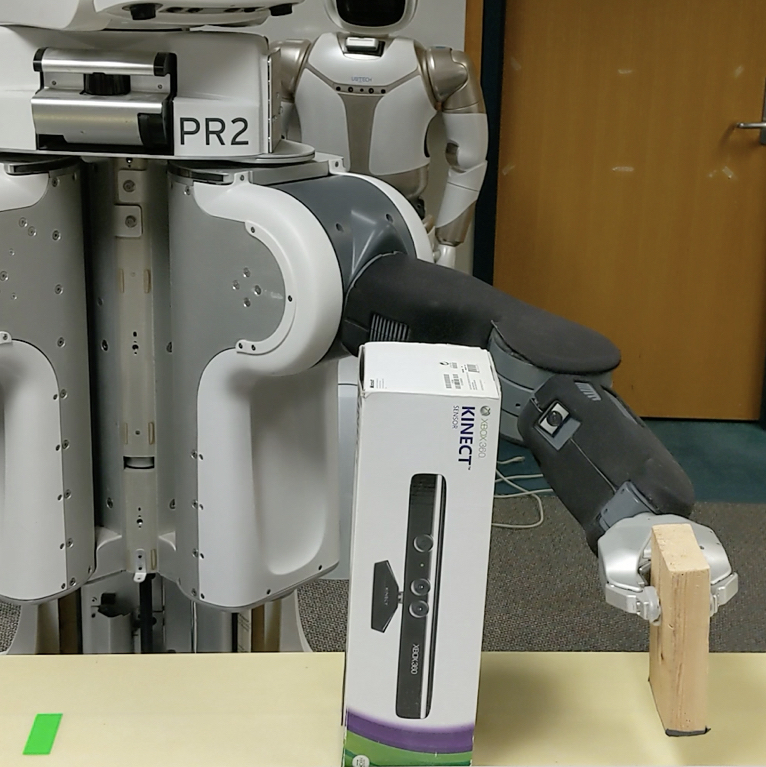
\includegraphics[width=\linewidth]{figures/cmax/pr2_pick_place_light_1_annotated.jpeg}
  \end{subfigure}
  \begin{subfigure}{0.24\linewidth}
    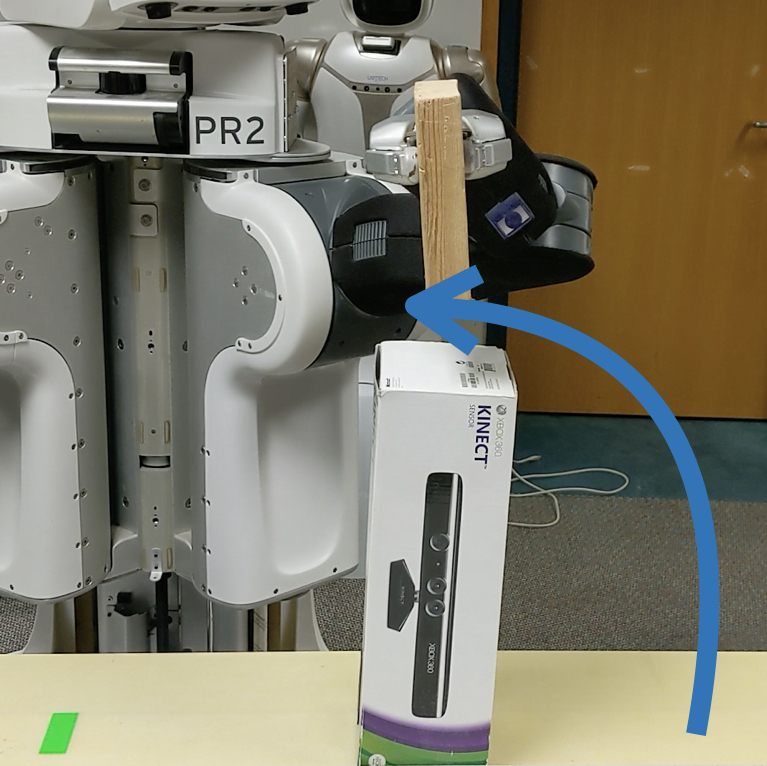
\includegraphics[width=\linewidth]{figures/cmax/pr2_pick_place_light_2_annotated.jpeg}
  \end{subfigure}
  \begin{subfigure}{0.24\linewidth}
    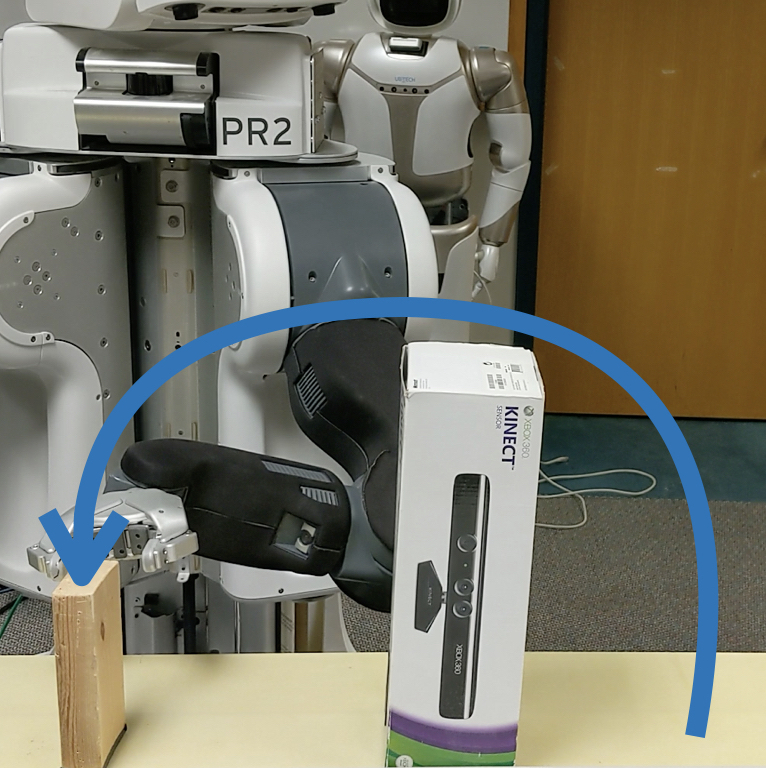
\includegraphics[width=\linewidth]{figures/cmax/pr2_pick_place_light_3_annotated.jpeg}
  \end{subfigure}
  \begin{subfigure}{0.24\linewidth}
    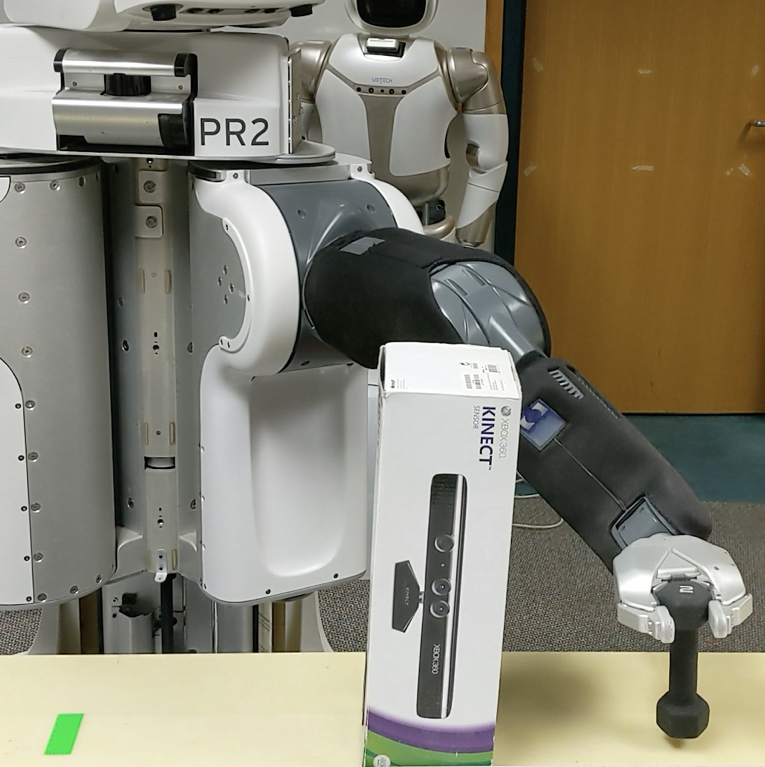
\includegraphics[width=\linewidth]{figures/cmax/pr2_pick_place_heavy_1_annotated.jpeg}
  \end{subfigure}
  \caption{A robotic arm picking an object from its start location and
  placing it at a goal location while avoiding collision with the
  intermediate obstacle during motion. The first three (from left)
  figures show an execution with a light object (wooden block) and a
  plan (blue trajectory) computed
  using an accurate dynamical model which captures the weight of the
  object correctly. The last figure (rightmost) shows an instance of
  the same task but with a heavy object (black dumbbell) and same
  dynamical model as before which models the object as light. This
  results in the planner computing the same plan as before, which the
  robot cannot execute as lifting the heavy object requires joint
  torques that are beyond the robot's capabilities. Thus, the plan is
  not task complete.}
  \label{fig:intro-example}
\end{figure*}
The above example highlights the ineffectiveness of naively using
these inaccurate models for planning. This ineffectiveness can be
tackled broadly in two directions: updating either the dynamical
model or the behavior of the planner, using the accumulated
experience during execution.

The former direction of using online
experience to update existing dynamical models or learning new
dynamical models from scratch has been explored in the Reinforcement
Learning (RL) framework. This framework enables autonomous agents,
such as robots, to learn how to operate in an unknown environment by
interacting with it and compute an optimal plan that minimizes total
cost~\cite{sutton1998introduction}. With partial or no prior knowledge
about the environment, the agent needs to explore to discover low cost
actions or regions where dynamics are inaccurately modeled. The
exploration strategies leveraged by these agents require a large
amount of interactions with the environment before we can compute
plans that guarantee task completeness. This is a major reason why RL,
despite being a very general framework, has mostly seen success in
domains where we can afford to collect large amounts of interactions
with little effort: video games and simulations.

Most methods in the RL framework can be categorized as either model-based
or model-free (Figure~\ref{fig:dyna}). As the name suggests, model-based methods rely on
using a model as input to a planning procedure to compute the solution
plan for a given task. These methods use the experience gained online
during execution to update the dynamics of the model and replan to
compute a new solution plan~\cite{DBLP:journals/sigart/Sutton91}. In
contrast, model-free methods directly 
use the accumulated experience to compute an updated solution plan
without ever using a dynamical model. These methods utilize the
experience to estimate value functions, which are esentially
cost-to-go estimates, and compute a plan using the estimated
values. Both methods have advantages and disadvantages. Model-based
methods relatively require fewer amounts of experience to compute a
plan of the same quality as the plan computed by a model-free
method. On the other hand, model-free methods are not affected by the biases
inherent in the design of the model.

\begin{figure}[t]
  \centering
  \includegraphics[width=0.5\linewidth]{Figures/intro/dyna.pdf}
  \caption{Operation of Model-based (blue) and Model-Free RL (red) methods
    while executing in unknown environments and collecting
    experience to complete a task. Figure inspired from Dyna~\cite{DBLP:journals/sigart/Sutton91}}
  \label{fig:dyna}
\end{figure}

In contrast, the latter direction of updating the behavior of the
planner using online experience has not been explored as extensively
in past literature. Interestingly, this direction has been explored by
the practitioner for quite some time. As motivated earlier, in most
robotic tasks we seldom have access to accurate dynamical models and
the models we use for planning are often inaccurate. Robotics
engineers and practitioners have been dealing with these inaccuracies
by modifying how the planner uses the inaccurate model rather than
updating the model to improve its accuracy. As an example, consider
the task of planning footsteps of a mobile quadruped robot over
partially unknown terrain as shown in Figure~\ref{fig:zucker} taken
from \cite{DBLP:journals/ijrr/ZuckerRSCBAK11}. The
unknown part of the terrain is annotated in the figure (red oval.) To
ensure that the planner does not compute footstep trajectory that goes
through this region, a simple
hack that the practitioner does is to inflate the cost of any
state-action pair that takes the robot into this region. This results
in biasing the planner away from this region thereby updating its
behavior. There are several other example applications where the
practitioner deals with inaccurate modeling by simply updating the
behavior of the planner. While this direction has been explored by the
practitioner, there is very little prior work that has studied this
direction from a theoretical point of view aiming to understand the
assumptions required to guarantee task completeness, and a systematic
study to analyze its empirical performance in practice. Our thesis
aims to fill this gap and develop a better understanding when, where
and how these methods work well in practice.

\section{Thesis Goal and Contributions}
\label{sec:thes-goal-contr}

While most existing works have presented and studied approaches that
use the experience from executions to update the dynamics of the
inaccurate model, one can argue that this is wasteful if we are interested in
completing the task and not in modeling the dynamics
accurately. Furthermore, robots operating in the real world have
operating constraints that require them to quickly adapt to
new scenarios and not spend hours acquiring experience to learn true
dynamics. In such spirit, our main focus in this thesis is to argue that by updating the
behavior of the planner and not the dynamics of the model, we can
leverage simplified and potentially inaccurate models and
significantly reduce the amount of real-world experience needed to
provably guarantee that the robot completes the task.

\begin{figure}[t]
  \centering
  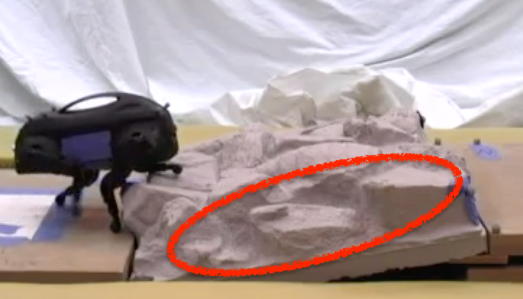
\includegraphics[width=0.5\linewidth]{Figures/intro/zucker}
  \caption{A practitioner's approach to dealing with inaccuracies in
    dynamical models used for planning. In this example, the robot is
    planning a footstep trajectory along the partially unknown terrain
  to reach the other side. The planner has access to a model of the
  terrain which is inaccurate in the regions marked by red oval. To
  ensure that the planner does not compute any trajectory going
  through the red oval region, practitioners typically inflate the
  cost of any action executed within the region or any action that
  takes the robot into this region. This results in biasing the
  planner away from this region thereby updating its behavior. Figure
  taken from \cite{DBLP:journals/ijrr/ZuckerRSCBAK11} and the red oval
  region depicted is an example used for emphasis.}
\label{fig:zucker}
\end{figure}

We support this argument by presenting two methods that update the
behavior of the planner and do not require any updates to the dynamics
of the inaccurate model used for planning.  Both methods come with
provable guarantees on completing the task under assumptions on the
accuracy of the model. In addition to these methods, we also emphasize
the importance of using simplified and inaccurate models for planning
by analyzing the sample complexity (or the amount of experience
needed) of exploration techniques used in model-free RL methods. Our
analysis shows that undirected global exploration techniques popularly
used in model-free RL methods can result in large sample complexity
requirements that cannot be realized in practice on a robot.

The primary contributions of this thesis can be detailed as follows.

\subsection{Sample Complexity of Exploration in Model-Free Policy
  Search}
\label{sec:sample-compl-expl}
We analyze the sample complexity of exploration techniques in
  model-free RL methods. This analysis is presented by viewing model-free policy
  search methods through the lens of derivative-free optimization (DFO)
  and computing upper bounds on the number of samples
  required to compute a $\epsilon$-suboptimal policy. We present a DFO
  point of view for methods that involve either exploration in action
  space or exploration in policy space, and present trade-offs between
  both styles of exploration in terms of the dimensionality of the
  policy parameter space, and the horizon length of the task. This
  analysis is presented in Chapter~\ref{cha:sample-compl-expl} of the  
  thesis and is also presented in our paper~\cite{aistats19}. In addition
  to contrasting exploration in policy space vs action space, this
  work also emphasizes the large sample complexity required by
  model-free methods, which cannot be realized in practice on a robot.
  
\subsection{Planning and Execution using Inaccurate Models}
\label{sec:plann-exec-using}
  We present the first systematic effort to understand methods
  that use online experience from executions to update the behavior of
  the planner and not update the dynamics of the model. Thus, these
  methods can make progress towards completing the task despite using
  a potentially inaccurate model. One can construct cases where if the
  model is highly inaccurate (e.g. a model that predicts a humanoid
  falling down for any action and failing to complete the task of
  moving forward,) then such a method cannot be expected to finish the
  task. Hence, we study the assumptions required on the accuracy of
  the model used for planning that ensures task completeness without
  requiring any updates to the dynamics of the model. Furthermore, we
  frame our problem in the purely online setting where the experience
  gathered by the robot is along a single trajectory without any
  access to resets. We believe that this setting is realistic and has
  challenges that these methods are uniquely positioned to tackle.

  We propose \cmax{}, an approach that guarantees that the robot
  completes the task using the inaccurate model without any resets and
  without requiring any updates to the dynamics of the model. This is
  achieved by biasing the planner away from transitions whose dynamics
  are discovered to be inaccurately modeled during online
  execution. On the theoretical side, we establish provable guarantees
  on task completeness under assumptions on the accuracy of the model
  used for planning. Empirically, we show that \cmax{} outperforms
  state-of-the-art model-free and model-based RL methods in terms of
  the number of executions taken to complete the task. Crucially,
  \cmax{} exhibits goal-driven behavior which enables it to focus on
  completing the task as quickly as possible and not waste executions  
  learning the true dynamics. This method is explained in detail in
  Chapter~\ref{cha:plann-exec} and is also presented in our
  paper~\cite{cmax}.

\subsection{Leveraging Experience in Planning and Execution using
  Inaccurate Models}
\label{sec:lever-exper-plann}
  
While a robot using \cmax{} is provably guaranteed to complete
  the task, it requires strong assumptions on the accuracy of the
  model that are often not realized in practice and hard to verify
  prior to execution. In addition for repetitive tasks, \cmax{} fails
  to improve the quality of the solution over repetitions of the same
  task as it does not leverage previously discovered inaccurately
  modeled transitions. This is remedied by our second approach
  \cmaxpp{} that leverages experience from past executions to improve
  the quality of solution over repetitions of the same
  task. Crucially, unlike \cmax{}, \cmaxpp{} can compute solution
  plans that contain previously discovered inaccurately modeled
  transitions. \cmaxpp{} achieves this by integrating model-free value
  learning using acquired experience with model-based planning using
  the inaccurate model. As a consequence of this in addition to
  completeness, \cmaxpp{} also guarantees asymptotic convergence to
  the optimal path cost as the number of repetitions increases. These
  guarantees of \cmaxpp{} are established under assumptions on the
  accuracy of the model that are much more relaxed compared to the
  assumptions required by \cmax{}. Importantly, like \cmax{},
  \cmaxpp{} never updates the dynamics of the model. This method is
  explained in detail in Chapter~\ref{cha:lever-exper} and is also 
  presented in our paper~\cite{cmaxpp}.

\section{Background}
\label{sec:background}

In this section, we provide background knowledge with the aim of
introducing classical techniques
that we will use throughout this thesis. Each chapter of this thesis
is self-contained and has detailed definitions that are more tailored
to the specific problem tackled in each chapter.

\subsection{Fundamentals of Markov Decision Processes}
\label{sec:fund-mark-decis}

In this thesis, we will primarily deal with finite horizon problems
where the objective is for an agent to minimize cumulative cost incurred over a
horizon of finite length. This is typically formulated as a finite horizon Markov
Decision Process (MDP)~\cite{bellman} that is represented as
$(\statespace, \actionspace, P, c, H)$ where $\statespace$ is the set
of states that the agent can be in, $\actionspace$ is the set of
actions that the agent can execute, $P$ is the transition dynamics
such that for any $s_t \in \statespace$, $s_{t+1} \in \statespace$,
$a_t \in \actionspace$, $P(s_{t+1}|s_t, a_t)$ is the probability of
transitioning to state $s_{t+1}$ from state $s_t$ by taking action
$a_t$, $c$ is the cost function such that for any transition $(s_t,
a_t)$, $c(s_t, a_t)$ is the cost incurred for that transition, and $H
\in \mathbb{N}^+$ is the length of the horizon. Typically, this
formulation also has a discounting factor $\gamma$ and a initial state
distribution $\rho$. In this thesis, we consider the non-discounted
setting where $\gamma = 1$ and a fixed initial state $s_0$ that is
known (thus, $\rho$ is a delta distribution on $s_0$.)

A deterministic policy $\pi: \statespace \rightarrow \actionspace$
maps from a state to an action. Given $\pi$ and a time step $t$, we can define the 
cost-to-go or value estimate $V_\pi^t(s)$ as follows:
\begin{equation}
  \label{eq:3}
  V_\pi^t(s) = \mathbb{E}\left[ \sum_{i=t}^H c(s_i, a_i) | a_i =
    \pi(s_i), s_{i+1} \sim P_{s_i, a_i}, s_t = s \right]
\end{equation}
where $P_{s_i, a_i} = P(\cdot|s_i, a_i)$ is a distribution over the
next state.

Similarly, we can also define the state-action value estimate
$Q_\pi^t(s, a)$ as follows:
\begin{equation}
  \label{eq:4}
  Q_\pi^t(s, a) = c(s, a) + \mathbb{E}_{s' \sim P_{s,a}}[V_\pi^{t+1}(s')]
\end{equation}

The objective function $J(\pi)$ is defined as
\begin{equation}
  \label{eq:6}
  J(\pi) = V_\pi^0(s_0)
\end{equation}
and the goal is to find a policy from a given policy set $\Pi$ that
minimizes the above objective function.

If the cost function and the transition dynamics is known, then one
can compute the optimal policy using Dynamic Programming (DP.) Denote
the optimal policy using $\pi^*$. Define $Q_{\pi^*}^{H-1}(s, a) = c(s,
a)$, we perform DP as follows: Starting from $t = H-2$ until $t = 1$
we iteratively do
\begin{align}
%  \label{eq:7}
  V_{\pi^*}^t(s) &= \max_{a \in \actionspace} Q_{\pi^*}^t(s, a) \\
  Q_{\pi^*}^{t-1}(s, a) &= c(s, a) + \mathbb{E}_{s' \sim P_{s, a}}[V_{\pi^*}^t(s')]
\end{align}
Given $Q_{\pi^*}^t$ we can compute the optimal action at time step $t$
and state $s_t$ 
as $\min_{a \in \actionspace} Q_{\pi^*}^t(s_t, a)$. The above
iterative process is called as Value Iteration. This iterative
procedures is derived by observing that the value function of the
optimal policy satisfies the following fixed point equation
\begin{equation}
  \label{eq:8}
  V_{\pi^*}^t(s) = \min_{a \in \actionspace} \left( c(s, a) + \mathbb{E}_{s'
  \sim P_{s,a}}[V_{\pi^*}^{t+1}(s')]\right)
\end{equation}
The above equation is known as the Bellman optimality condition.

\subsection{Deterministic Shortest Path Problem}
\label{sec:determ-short-path}

The shortest path problem is to find among all paths that start at a
given state and end at a goal state, a path has the minimum cost; this
is also called a shortest path~\cite{bertsekas1995neuro}. This can be instantiated as a markov
decision process represented using the tuple $(\statespace,
\actionspace, \goalspace, f, c)$ where $\goalspace \subseteq
\statespace$ is the set of goal states, and $f:\statespace \times
\actionspace \rightarrow \statespace$ is a deterministic
dynamics function that determines the successor state $s_{t+1}$ of a
transition $(s_t, a_t)$ as $f(s_t, a_t)$. The goal states in
$\goalspace$ are cost-free termination states, i.e. $f(g, a) = g$, $c(g,
a) = 0$ for
all $g \in \goalspace$ and any action $a \in \actionspace$. We also
assume that the cost of any transition starting from a non-goal state
is positive, i.e. $c(s, a) > 0$ for all $s \in \statespace \setminus
\goalspace$ and $a \in \actionspace$.

We are interested in problems where reaching the termination state is
inevitable, at least under an optimal policy. Thus, the essence of the
problem is how to reach a goal state with minimum cost. In the
shortest path problem setting, we use $V(s)$ to denote the cost-to-go
(or value) estimate of any state $s \in \statespace$ and $V^*(s)$ to
denote the optimal cost-to-go (or value.) From the Bellman optimality
condition we know
\begin{equation}
  \label{eq:9}
  V^*(s) = \min_{a \in \actionspace}\left( c(s, a) + V^*(f(s, a)) \right)
\end{equation}
A value estimate $V$ is called admissible if underestimates the
optimal value at all states, i.e. $V(s) \leq V^*(s)$ for all $s \in
\statespace$. Furthermore, $V$ is called consistent if it satisfies
the condition that for any state-action pair $(s, a)$, $s \notin
\goalspace$, $V(s) \leq c(s, a) + V(f(s, a))$ and $V(g) = 0$ for all
$g \in \goalspace$.
A typical assumption made in all shortest path problems is that there
exists at least one path from each state $s \in \statespace$ to one of
the goal states in $\goalspace$. This ensures that the optimal value
for any state is finite.

\subsection{Real-time Heuristic Search}
\label{sec:real-time-heuristic-1}

A traditional way to solve the shortest path problem is to search the
graph constructed using a mental model of the world, and then
subsequently execute the resulting plan (or follow the computed path.)
Thus, planning and execution are completely separated. An alternative
way of solving this problem is to search online by interleaving
planning and execution which results in several advantages with the
major advantage being drastic reductions in planning time. This is
achieved by performing search locally until a fixed horizon (or until
a fixed number of states are expanded,) and then execute the best
action for the current state. After the execution, planning is
performed once again to find the next best action. This can decrease
the time used for planning as we are not planning all the way to the
goal. Another significant advantage is when the mental model of the
world is inaccurate, these methods enable the agent to update its
model and ensure future replanning results in more optimal paths.

Since the future consequences of executed actions are unknown,
interleaving planning and execution can result in slight overhead in
terms of the number of actions executed but this is often a much
smaller overhead compared to the reduced planning time. Real-time
search methods are methods that interleave planning and execution by
searching forward from the current state of the agent. Most
importantly, real-time heuristic search methods can satisfy hard
real-time requirements in large state spaces since the sizes of their
local search spaces are independent of the sizes
of the state spaces and can thus remain small. 

In this thesis, we will focus on Learning real-time A* (LRTA*) real-time search methods
that are real-time search methods that associate information with the
states to prevent cycling. These methods are promising for
interleaving planning and execution as they are efficient
domain-independent search methods that allow fine-grained control over
how much planning is allowed between executions, use heuristic
knowledge to guide planning, and improve their performance over time
as they solve similar planning tasks. LRTA* operates on deterministic
domains only.

\begin{algorithm}[t]
  \caption{LRTA* with Lookahead $1$~\cite{DBLP:journals/ai/Korf90}}
  \begin{algorithmic}[1]
    \State $s \leftarrow s_0$
    \While{$s \notin \goalspace$}
    \State Compute action $a = \argmin_{a \in \actionspace} \left( c(s, a) +
      V(f(s, a)) \right)$
    \State Update $V(s) \leftarrow \min\left( V(s), c(s, a) + V(f(s,
      a)) \right)$
    \State Execute action $a$ and update $s \leftarrow f(s, a)$
    \EndWhile
  \end{algorithmic}
  \label{alg:lrta}
\end{algorithm}

Algorithm~\ref{alg:lrta} presents the LRTA* algorithm for a lookahead
or search horizon of $1$. At each time step, the algorithm looks one
action execution ahead and always greedily chooses the action that
leads to a successor state with the minimum sum of cost of
transitioning into the successor state and the value estimate of the
successor state. Furthermore unlike classical real-time search
methods, LRTA* also updates the value estimates of the current state
to reflect the updated estimate of the best path to the goal so that
future replanning is more efficient. The planning time of LRTA*
between executions is linear in the number of actions. If the size of
action space is independent of the size of state space, then the
planning time is independent of the size of state space which is a
major improvement over offline planning methods whose computational
complexity is at most the size of the state space.

LRTA* can be viewed as a form of asynchronous incremental dynamic
programming method~\cite{DBLP:journals/ai/BartoBS95}. It can be shown
that LRTA* is guaranteed to reach a goal state in a finite number of
executions and if we reset to the start state after reaching the goal
state, then the value estimates eventually converge to the optimal
value function~\cite{DBLP:journals/ai/Korf90}. These guarantees hold
under the assumption that the initial value estimates that we start
with are admissible and consistent. These assumptions are very similar
to the traditional definitions of admissible and consistent heuristic
values for A* search. Note that zero-initialized value estimates are
both admissible and consistent.

Real-time Adaptive A* (RTAA*) proposed
in~\cite{DBLP:conf/atal/KoenigL06} is similar to LRTA*
(Algorithm~\ref{alg:rtaa}). They only 
differ in the way they update the
value estimates at each time step. To understand this better, let us
look at how LRTA* updates value estimates. LRTA* replaces the value
estimate of each expanded state with the sum of costs of from the
state to a generated but unexpanded state $s$ (leaf node in the search
tree) and the value estimate of state $s$, minimized over all
generated but unexpanded states (all leaf nodes of the search tree.)
If we denote $V$ as the value estimates after all the value
updates then the LRTA* updates satisfy the following system of
equations for all expanded states $s$:
\begin{equation}
  \label{eq:10}
  V(s) = \min_{a \in \actionspace}\left( c(s, a) + V(f(s, a)) \right)
\end{equation}

\begin{algorithm}[t]
  \caption{RTAA* with lookahead $K \geq 1$}
  \begin{algorithmic}[1]
    \State $s \leftarrow s_0$
    \While{$s \notin \goalspace$}
    \State Construct a search tree at $s$ until $K$ expansions
    \State Estimate $\bar{s}$ as the leaf node with the least $g + V$
    estimate among all leaf nodes
    \For{all expanded states $s'$}
    \State Update $V(s') \leftarrow g(\bar{s}) + V(\bar{s}) - g(s')$
    \EndFor
    \State Compute action $a$ as the first action on the path from
    state $s$ to state $\bar{s}$ in the search tree
    \State Execute action $a$ and update $s \leftarrow f(s, a)$
    \EndWhile
  \end{algorithmic}
  \label{alg:rtaa}
\end{algorithm}

On the other hand, RTAA* constructs a search tree very similar to
LRTA* (the number of states expanded is equal to the lookahead) but
updates the value estimates for all expanded states $s$ as follows:
\begin{equation}
  \label{eq:11}
  V(s) = g(\bar{s}) + V(\bar{s}) - g(s)
\end{equation}
where $g(s)$ encodes the cost-to-come from the root of the search tree
to the state $s$ (i.e. sum of costs of all transitions on the path
from root to state $s$,) and $\bar{s}$ is the state corresponding to
the leaf node with the least sum of $g$ and $V$ among all leaf nodes
in the search tree. In other words, $\bar{s}$ is the state that was
about to be expanded just before the search was terminated. One can
show that LRTA* and RTAA* updates are exactly the same when the
lookahead is $1$. But when the lookahead is greater than $1$, these
updates differ. More specifically, LRTA* updates tend to be more
informed or reflect the optimal cost-to-go better when compared to
RTAA* updates. However, it takes LRTA* more time to update the value
estimates and is difficult to implement. This is because LRTA*
performs one search to determine the local search space and a second
search to determine how to update the value estimates since it is
unable to use the results from the first search for this
purpose. Thus, there is a trade-off between the total search time and
cost of the resulting path. In practice, for lookaheads greater than
$1$, RTAA* tends to compute solution paths that have higher costs
compared to LRTA* but the time taken for planning before each execution is
significantly less in RTAA* compared to LRTA*. This makes RTAA*
desirable in applications where planning is slow but actions can be
executed fast and there is a very strict time limit per search episode.

\subsection{Local Function Approximation Methods}
\label{sec:local-funct-appr-1}



%%% Local Variables:
%%% mode: latex
%%% TeX-master: "../main"
%%% End:


\chapter{Background}
\label{cha:background}


%%% Local Variables:
%%% mode: latex
%%% TeX-master: "../main"
%%% End:


\chapter{Related Work}
\label{cha:related-work}

\epigraph{\textit{If I have seen further it is by standing on the
    shoulders of Giants.}}{Isaac Newton (1676)}

This chapter presents existing literature that is relevant
to the research problems tackled in this
thesis. Section~\ref{sec:expl-model-free} outlines past work in
model-free reinforcement learning that introduced different
exploration techniques. Prior works on real-time heuristic search
methods, that are extensively used 
in this thesis, are presented in
Section~\ref{sec:real-time-heuristic}. Local function approximation
techniques have been very successful in robotics and some example
works are introduced in
Section~\ref{sec:local-funct-appr}. Section~\ref{sec:model-based-reinf}
outlines existing literature on model-based reinforcement learning
methods which combine learning dynamical models online with model-based
planning using the learned models.
Very recent works that have proposed approaches integrating
model-free learning with model-based planning are highlighted in
Section~\ref{sec:integr-model-free}. Finally,
Section~\ref{sec:using-inacc-models} presents prior work in
reinforcement learning and planning communities that utilize
inaccurate models to reduce the amount of real-world experience
required to compute a successful plan or an optimal policy. In all
these domains, the amount of literature is immense so the focus in
this chapter is on relevance to this thesis rather than an exhaustive list.

\section{Exploration in Model-Free RL}
\label{sec:expl-model-free}

% Mention greedy approaches - estimate model and then exploit it fully
% Why exploration is really needed
% Mention that in model-based learning, we can do more intelligent
% exploration such as E3 and RMAX
% But in model-free, broadly two categories

\subsection{Exploration in Action Space}
\label{sec:expl-acti-space}

\subsection{Exploration in Policy Space}
\label{sec:expl-policy-space}


\section{Real-time Heuristic Search}
\label{sec:real-time-heuristic}

% LRTA*, RTAA*, RTDP, vadim bulitko's paper
% weighted real-time heuristic search

\section{Local Function Approximation Methods}
\label{sec:local-funct-appr}

% CHris Atkeson's papers, LWR, LWPR
% Inverse dynamics learning papers from Schaal 

\section{Model-based RL with Provable Guarantees}
\label{sec:model-based-reinf}

% E3, RMAX, MBIE, C-PACE, Adaptive resolution, Sham's thesis,
% 

\section{Integrating Model-Free and Model-Based Learning}
\label{sec:integr-model-free}

% CMAX++ references (Lagrassa , Lee papers and their references),
% Not so much work

\section{Using Inaccurate Models in Planning and Execution}
\label{sec:using-inacc-models}

% Abbeel paper, ILC, PAC RL Jiang paper, Dale McConcachie, Offline RL,
% Residual Model learning papers




%%% Local Variables:
%%% mode: latex
%%% TeX-master: "../main"
%%% End:


\chapter{Sample Complexity of Exploration in Model-Free Policy Search}
\label{cha:sample-compl-expl}

\epigraph{\textit{... much of the benefit of policy search is achieved
by black-box methods.}}{Jens Kober, Drew Bagnell and Jan Peters (2013)}

\section{Introduction}
Model-free policy search is a general approach to learn parameterized
policies from sampled trajectories in the environment without
learning a model of the underlying dynamics. These methods
update the parameters such that trajectories with higher returns (or total reward) are
more likely to be obtained when following the updated policy
\citep{kober2013reinforcement}. The simplicity of these approaches have
made them popular in Reinforcement Learning (RL).

Policy gradient methods, such as REINFORCE \citep{williams1992simple}
and its extensions \citep{kakade2002natural,bagnell2004policy, silver2014deterministic,schulman2015trust},
compute an estimate of a direction of improvement from sampled
trajectories collected by executing a stochastic policy. In other words, these methods rely on
randomized exploration in action space. These methods then leverage
the Jacobian of the policy to update its parameters to increase the
probability of good action sequences accordingly. Such a gradient
estimation algorithm can be considered a combination of a
\textit{zeroth-order} approach and a \textit{first-order} approach:
(1) it never exploits the slope of the reward function or dynamics,
with respect to actions, but rather relies only on random exploration
in action space to discover potentially good sequences of actions; (2)
however, it \emph{exploits} the first order information of the
parameterized policy for updating the policy's parameters. Note that
the chance of finding a sequence of actions resulting in high total
reward decreases (as much as exponentially
\citep{kakade2002approximately}) as the horizon length increases and
thus policy gradient methods often exhibit high variance and a
resulting large sample complexity \citep{peters2008reinforcement,
  zhao2011analysis}.

Black-box policy search methods, on the other hand, seek to directly
optimize the total reward in the space of parameters by employing
, e.g., finite-difference-like methods to compute estimates of the
gradient with respect to policy parameters
\citep{bagnell2001autonomous,mannor2003cross,heidrich2008evolution,tesch2011using,sehnke2010parameter,salimans2017evolution,mania2018simple}.  
Intuitively, these methods rely on exploration in parameter space: by
searching in the parameter space, these methods may discover an
improvement direction. Note that these methods are fully zeroth-order,
\textit{i.e.}, they exploit no first-order information of the
parameterized policy, the reward, or the dynamics.  Although policy gradient methods leverage \textit{more} information,
notably the Jacobian of the action with respect to policy, black-box policy search methods have
at times demonstrated better empirical performance (see the discussion in 
\citep{kober2013reinforcement, mania2018simple}). These perhaps surprising results motivate us to analyze:
\textit{In
  what situations should we expect parameter space policy search methods
  to outperform action space methods?}

To do so, we leverage prior work in zeroth-order
optimization methods. In the convex setting, 
\citep{flaxman2005online, agarwal2010optimal, nesterov2017random}
showed that one can construct %
gradient %
estimates using zeroth order oracles and derived upper bounds on the
number of samples needed. 
%
%
%
But for most RL tasks,
the return as a function of parameters, or action sequence, is highly
non-convex \citep{sutton1998introduction}. Hence we focus on the non-convex setting and analyze convergence to stationary points. \cite{ghadimi2013stochastic, nesterov2017random} studied zeroth order
non-convex optimization by providing upper bounds on
the number of samples needed to close in on a stationary
point. Computing lower bounds in zeroth order non-convex optimization is still
an open problem %
%
\citep{carmon2017lower, carmon2017lower2}. 

In our work, we extend the analysis proposed in \citep{ghadimi2013stochastic} to the policy search setting 
%
%
and analyze the sample complexity of parameter and action space exploration methods in policy search. We begin with a degenerate, one-step control problem of online linear regression with partial feedback, \citep{flaxman2005online}, where the objective is to learn the parameters of the linear regressor without access to the true scalar regression targets. We show that for parameter space exploration methods, to achieve $\epsilon$-optimality, requires $O(b^2/\epsilon^4)$ samples, 
%
where $b$ is the input feature dimensionality. By contrast, an action space exploration method requires $O(1/\epsilon^4)$ many samples
%
with a sample complexity \textit{independent} of input feature dimensionality $b$. %
This is tested empirically on two simple tasks:  Bandit Multi-class learning on MNIST with policies parameterized by convolutional neural networks which can be seen as a Contextual Bandit problem with rich observations, and Online Linear Regression with partial information. The results demonstrate action space exploration methods outperform  parameter space methods when the parameter dimensionality is substantially larger than action dimensionality.

We present similar analysis for the multi-step control problem of model-free policy search in reinforcement learning, \citep{kober2013reinforcement}, by considering the objective of reaching $\epsilon$-close to a stationary point in the sense that $\|\nabla J(\theta)\|_2^2 \leq \epsilon$ for the non-convex objective $J(\theta)$. Our results show that, under certain assumptions, parameter space exploration methods 
%
need $\mathcal{O}(\frac{d^2}{\epsilon^3})$ samples to reach $\epsilon$ close to a stationary point, where $d$ is the policy parameter dimensionality. On the other hand, action space exploration methods need $\mathcal{O}(\frac{p^2H^4}{\epsilon^4})$ samples to achieve the same objective, where $p$ is the action dimensionality and $H$ is the horizon length of the task. This shows that action space exploration methods have a dependence on the horizon length $H$ %
while parameter space exploration methods depend only on parameter space dimensionality $d$.
%
Ongoing work by \cite{tu2018gap} demonstrated through asymptotic lower bounds that the dependence of sample complexity of action space exploration methods on horizon $H$ is unavoidable in the LQR setting.
This is tested empirically on popular RL benchmarks from OpenAI gym \citep{openaigym}, and the results show that as horizon length increases, parameter space methods outperform action space exploration methods. This matches the intuition and results presented in recent works like \citep{bagnell2001autonomous,szita2006learning,tesch2011using,salimans2017evolution, mania2018simple}
%
that show parameter space black-box policy search methods outperforming state-of-the-art action space methods for tasks with long horizon lengths.

In summary, our analysis and experimental results suggests that the
complexity of exploration in action space depends on both the
dimensionality of action space and \emph{horizon}, while the
complexity of exploration in parameter space solely depends on
dimensionality of parameter space, providing a natural way to trade-off
between these approaches.

%
%
%

%

%
%
%


%

%

%

\section{Problem Setup}
\label{sec:problem_define}


\subsection{Multi-step Control: Reinforcement Learning}
\label{sec:rl-problem}
We consider the problem setting of model-free policy search with the goal of
minimizing sum of costs (or maximizing sum of rewards) over a fixed,
finite horizon $H$. In reinforcement learning (RL), this is typically
formulated using Markov Decision Processes (MDP)
\citep{sutton1998introduction}. Denote the state space of the MDP as
$\mathcal{S} \subset 
\mathbb{R}^b$, action space as $\mathcal{A} \subset  \mathbb{R}^p$
, transition probabilities as
$\mathbb{P}_{sa} = \mathbb{P}(\cdot|s, a)$ (which is the distribution of next state after
executing action $a \in \mathcal{A}$ in state $s \in \mathcal{S}$), an
initial state distribution $\mu$, and a cost function $c(s,a) :
\mathcal{S} \times \mathcal{A} \rightarrow \mathbb{R}$. Note that the
cost can be interpreted as negative of the reward. In addition to
this, we assume a restricted class of deterministic, stationary
policies $\Pi$ parameterized by $\theta \in \mathbb{R}^d$ where each
$\pi(\theta, \cdot) \in \Pi$ is differentiable at all $\theta$ and is a mapping from $\mathcal{S}$ to
$\mathcal{A}$, i.e. $\pi(\theta, \cdot): \mathcal{S} \rightarrow
\mathcal{A}$. The distribution of states at timestep $t$ induced by
running the policy $\pi(\theta, \cdot)$ until and including $t$, is
defined $\forall s_t: d_{\pi_\theta}^t(s_t) = \sum_{\{s_i\}_{i \leq
    t-1}} \mu(s_0) \prod_{i=0}^{t-1} \mathbb{P}(s_{i+1}|s_i, a_i =
\pi(\theta, s_i))$, where by definition $d_{\pi_\theta}^0(s) = \mu(s)$
for any $\pi$. We define the value function $V^t_{\pi_\theta}(s)$ for $t \leq H-1$ as 
%
\begin{equation*}
  V^t_{\pi_\theta}(s) = \mathbb{E}[\sum_{i=t}^H c(s_i, \pi(\theta,
s_i))|s_t = s]
\end{equation*}
and state-action value function $Q^t_{\pi_\theta}(s, a)$ as
\begin{equation*}
  Q^t_{\pi_\theta}(s, a) = c(s, a) + \mathbb{E}_{s' \sim
                           \mathbb{P}_{sa}}[V^{t+1}_{\pi_\theta}(s')]
\end{equation*}
Throughout this work, we assume the total cost is upper bounded by a constant, i.e., $\sup_{c_1,\dots, c_T}\sum_{t} c_t \leq \Qbound\in\mathbb{R}^+$, to prevent confounding due to just a change in the scale of total costs. We have then that $Q^t_{\pi_\theta}$ is upper bounded by a constant $\Qbound$ for all $t$ and $\theta$.

We seek to minimize
the performance objective given by $J(\theta) = \mathbb{E}_{s \sim
  \mu}[V^0_{\pi_\theta}(s)]$. Given this
objective, the optimization problem  can be formulated
as:
\begin{equation}
  \label{eq:1}
  \min_\theta J(\theta)
\end{equation}
The goal is to find parameters $\theta^*$ that minimize the
expected sum of costs $J(\theta)$, given no access to the underlying dynamics
of the environment other than samples from the distribution
$\mathbb{P}_{sa}$ by executing the policy $\pi(\theta,
\cdot)$. However, the objective $J(\theta)$ can be highly non-convex
and finding a global minima could be intractable. Thus, in this work, we hope to find a stationary point
$\theta^*$ of the objective $J(\theta)$, \textit{i.e.} a point where
$\nabla_\theta J(\theta) \approx 0$.

 
%


\subsection{One-Step Control: Online Linear Regression with Partial Information}
\label{sec:define_OLR}
The online linear regression problem is defined as follows: We denote
$\mathcal{S}\subset\mathbb{R}^{b}$ as the feature space, and $\Theta
\subset\mathbb{R}^{d} = \mathbb{R}^b$ as the linear policy parameter space where each
$\theta\in\Theta$ represents a policy $\pi(\theta, s) =
\theta^{\top}s$. Online linear regression operates in an adversarial
online learning fashion: every round $i$, nature presents a
feature vector $s_i\in\mathcal{S}$, the learner makes a decision by
choosing a policy $\theta_{i}\in\Theta$ and predicts the scalar action
$\hat{a}_i = \theta_i^{\top}s_i$; nature then reveals the loss
$(\hat{a}_i - a_i)^2 \in\mathbb{R}^+$, which is just a scalar, to the
learner, where $a_i$ is ground truth selected by nature and is
never revealed to the learner.  We do not place any statistical
assumption on the nature's process of generating feature vector $s_i$
and ground truth $a_i$, which could be completely adversarial. Other
than the adversarial aspect of the problem, note that the above setup
is a special setting of RL with horizon $H=1$, linear policy
$\theta^{\top}s_i$, one-dimension action space, and a cost function
$c_i(\theta) = (\theta^{\top}s_i - a_i)^2$. In this setting, we
consider the \textit{regret} with respect to the optimal solution in hindsight,
\begin{align}
    \mathrm{Regret} = \sum_{i=1}^{T} c_i(\theta_i) - \min_{\theta^\star\in\Theta} \sum_{i=1}^T c_i(\theta^\star)
\end{align}
%

\section{Online Linear Regression with Partial Information}
\label{sec:olr}
%
 

\subsection{Exploration in Parameter Space}
We can apply a zeroth-order
online gradient descent algorithm for the sequence of loss functions
$\{c_i\}_{i=1}^T$, which is summarized in
Algorithm~\ref{alg:random_search_OLR}. The main idea is to add random
noise $u$, sampled from a unit sphere in $b$-dim space $\mathbb{S}_{b}$, to the parameter $\theta$, and querying loss at $\theta+\delta u$ for some $\delta > 0$. Using the received loss $c_i(\theta+\delta u)$, one can form an estimation of $\nabla_{\theta}c_i(\theta)$ as $\frac{c_i b}{\delta}u$ \citep{flaxman2005online}. 

%

\begin{algorithm}[ht]
\caption{Random Search in Parameter Space (BGD \cite{flaxman2005online})}
 \label{alg:random_search_OLR}
\begin{algorithmic}[1]
  \State {\bfseries Input:} $\alpha\in\mathbb{R}^+$, $\delta\in\mathbb{R}^+$.
  \State Learner initializes $\theta_1\in\Theta$.
  \For {$i = 1$ to $T$}
    \State Learner samples $u\sim \mathbb{S}_{b}$. 
    %
    \State Learner chooses predictor $\theta_i' = \theta_i + \delta u$. 
    \State Learner only receives loss signal $c_i(\theta_i')$. %
    \State Learner update: $\theta_{i+1}' = \theta_i - \alpha \frac{c_i b}{\delta}u$.
    \State Projection $\theta_{i+1} = \arg\min_{\theta\in{\Theta}}\|\theta_{i+1}'-\theta\|_2^2$.
  \EndFor
\end{algorithmic}
\end{algorithm}


\subsection{Exploration in Action Space}
The \emph{key difference} between exploration in action space and exploration in parameter space is that we are going to leverage our knowledge of the policy $\pi(\theta, s) = \theta^{\top} s$. Since we design the policy class, we can compute its \emph{Jacobian} with respect to its parameters $\theta$ without interaction with the environment. The Jacobian of the policy gives us a locally linear relationship between a small change in parameter and the resulting change in policy's action space. The main idea then in this approach is to explore with randomization in action space, and then leverage the Jacobian of the policy to update the parameters $\theta$ accordingly so that the policy's output moves towards better actions. Intuitively, we expect that random exploration in action space will result in smaller regret, as in our setting the action space is just $1$-dimensional, while the parameter space is $b$-dimensional.  %
The approach is summarized in Algorithm~\ref{alg:random_search_action_olr}. Denote $\ell_i = (\hat{a}_i - a_i)^2$ and $\hat{a}_i = \pi(\theta_i, s_i) = \theta_i^{\top}s_i$. The main idea is that we can compute $\nabla_{\theta} c_i(\theta_i)$ via a chain rule as $\nabla_{\theta} c_i (\theta_i) = \frac{\partial{\ell_i}}{\partial{\hat{a}_i}}\nabla_{\theta}\pi(\theta_i, s_i)$. Note that $\nabla_{\theta}\pi(s_i, \theta_i) = \nabla_\theta \theta_i^{\top}s_i = s_i$ is the Jacobian of the policy to which we have full access. We then use zeroth order approximation method to approximate $\partial{\ell_i}/\partial{\hat{a}_i}$ at $\hat{a}_i = \pi(\theta_i, s_i)$.


\begin{algorithm}[ht]
\caption{Random Search in Action Space}
 \label{alg:random_search_action_olr}
\begin{algorithmic}[1]
  \State {\bfseries Input:} $\alpha\in\mathbb{R}^+$, $\delta\in\mathbb{R}^+$.
  \State Learner initializes $\theta_1\in\Theta$.
  \For {$i = 1$ to $T$}
    \State Learner receives feature $s_i$.
    \State Learner samples $e$ uniformly from $\{-1,1\}$.
    \State Learner makes a prediction $\hat{a}_i = \theta_i^{\top} s_i + \delta e$
    \State Learner only receives loss signal $c_i = (\hat{a}_i - a_i)^2$. %
    \State Learner update: $\theta_{i+1}' = \theta_i - \alpha \frac{c_i e}{\delta}s_i$.
    \State Projection $\theta_{i+1} = \arg\min_{\theta\in{\Theta}}\|\theta_{i+1}'-\theta\|_2^2$.
  \EndFor
\end{algorithmic}
\end{algorithm}


\subsection{Analysis}
We analyze the regret of the exploration in parameter space algorithm (Alg.~\ref{alg:random_search_OLR}) and the exploration in action space algorithm (Alg.~\ref{alg:random_search_action_olr}) in this section. For analysis, we assume that $\Theta$ is bounded, i.e., $\sup_{\theta\in\Theta}\|\theta\|_2 \leq C_{\theta}\in\mathbb{R}^+$, $\mathcal{S}$ is bounded, i.e., $\sup_{s\in\mathcal{S}}\|s\|_2 \leq C_s\in\mathbb{R}^+$, and the ground truth $a_i$ is bounded, i.e., $|a_i|\leq C_{a}$ for any $i$. Under the above assumptions, we can make sure that the loss is bounded as well, $(\theta^{\top}s - a)^2 \leq C\in\mathbb{R}^{+}$. The loss function is also Lipschitz continuous with Lipschitz constant $L \leq (C_{\theta}C_{s} + C_{a})C_{s}$. We call these constants $C_{s}, C_{\theta}$, and $C_{a}$ as problem dependent constants, which are independent of feature dimension $b$ and number of rounds $T$.
%
In regret bounds, we absorb problem dependent constants into $\mathcal{O}$ notations, but the bounds will be explicit in $b$ and $T$. The theorem below presents the average regret analysis for these methods,

\begin{theorem}
After $T$ rounds, %
%
%
%
%
with $\alpha = \frac{{C_{\theta}}\delta}{b(C^2+C_{s}^2)\sqrt{T}}$ and $\delta = T^{-0.25}\sqrt{\frac{C_{\theta}b(C^2+C_{s}^2)}{2L}}$, Alg.~\ref{alg:random_search_OLR} incurs average regret:
\begin{align}
\label{eq:random_para}
    \frac{1}{T}(\mathbb{E}[\sum_{i=1}^T c_i(\theta_i)] - \min_{\theta^\star
  \in \Theta}\sum_{i=1}^T c_i(\theta^\star)) \leq %
    \mathcal{O}(\sqrt{b}T^{-\frac{1}{4}}),
\end{align}
and with $\alpha = \frac{C_{\theta}\delta}{(C^2+1)C_{s}\sqrt{T}}$ and $\delta = T^{-0.25}\sqrt{\frac{C_{\theta}(C^2+1)C_{s}}{2C}}$, Alg.~\ref{alg:random_search_action_olr} incurs average regret:
\begin{align}
\label{eq:random_action}
    \frac{1}{T}(\mathbb{E}[\sum_{i=1}^T c_i(\theta_i)] -
  \min_{\theta^\star \in \Theta}\sum_{i=1}^T c_i(\theta^\star)) \leq %
    \mathcal{O}(T^{-\frac{1}{4}}),
\end{align} for any $\theta\in\Theta$.
\label{thm:online_linear_regression}
\end{theorem}

The proof for the above theorem can be found in our original paper~\cite{aistats19}.

The above regret analysis essentially shows that exploration in action space delivers a regret bound that is independent of parameter space dimension $b$, while the regret of the exploration in parameter space algorithm will have explicit polynomial dependency on feature dimension $b$.  Converting the regret bounds to sample complexity bounds, we have that for any $\epsilon\in (0,1)$, to achieve $\epsilon$-average regret, Alg.~\ref{alg:random_search_OLR} needs $\mathcal{O}(\frac{b^2}{\epsilon^4})$ many rounds, while Alg.~\ref{alg:random_search_action_olr} requires $\mathcal{O}(1/\epsilon^4)$ many rounds.  

Note that in general if we have a multivariate regression problem, i.e., $a\in\mathbb{R}^{p}$, regret of Algorithm~\ref{alg:random_search_action_olr} will depend on $\sqrt{p}$ as well. But from our extreme case with $p=1$, we clearly demonstrate the sharp advantage of exploration in action space: \emph{when the action space's dimension is smaller than the dimension of parameter space}, we should prefer the strategy of exploration in action space.




\section{Reinforcement Learning}
\label{sec:RL}

In this section, we study exploration in parameter space versus exploration in action space for multi-step control problem of model-free policy search in RL. As explained in Section~\ref{sec:problem_define}, we are interested in rates of convergence to a stationary point of $J(\theta)$.

\subsection{Exploration in Parameter Space}
\label{sec:parameter_space}
The objective defined in Section \ref{sec:rl-problem} can be optimized
directly over the space of parameters $\mathbb{R}^d$. Since we do not use first-order (or gradient) information about the
objective, this is equivalent to derivative-free (or zeroth-order)
optimization with noisy function evaluations. More specifically, for a parameter vector
$\theta$, we can execute the corresponding policy $\pi(\theta, \cdot)$
in the environment, to obtain a noisy estimate of $J(\theta)$. This
noisy function evaluation can be used to construct a gradient estimate
and an iterative stochastic gradient descent approach can be used to
optimize the objective. An algorithm that closely follows the ones
proposed in \citep{agarwal2010optimal, mania2018simple}
 and optimizes over the space of parameters  is shown in Algorithm
\ref{alg:random_search_parameter}. Since we are working in episodic RL setting, we can use a two-point estimate to form a gradient estimation (Line 7 \& 8 in Alg.~\ref{alg:random_search_parameter}), which in general will reduce the variance of gradient estimation \citep{agarwal2010optimal}, compared to one-point estimates.
\begin{algorithm}[ht]
\caption{Policy Search in Parameter Space}
 \label{alg:random_search_parameter}
\begin{algorithmic}[1]
  \State {\bfseries Input:} Learning rate $\alpha \in\mathbb{R}^+$, standard deviation of exploration noise $\delta\in\mathbb{R}$
  \State Initialize parameters $\theta_1\in\mathbb{R}^d$
  \For {$i = 1$ to $T$}
    \State Sample $u \sim \mathbb{S}_d$ , a $d$-dimensional unit sphere
    \State Construct parameters $\theta_i + \delta u$, $\theta_i - \delta u$
    \State Execute policies $\pi({\theta_i + \delta u}, \cdot),
    \pi({\theta_i - \delta u}, \cdot)$ 
    \State Obtain noisy estimates of the objective $J^+_i = J(\theta_i
    + \delta u) + \eta^+_i$ and $J^-_i = J(\theta_i - \delta u) +
    \eta^-_i$ where $\eta^+_i, \eta^-_i$ are zero mean random i.i.d noise
    \State Compute gradient estimate $g_i = \frac{d(J^+_i - J^-_i)}{2\delta} u $
    \State Update $\theta_{i+1} = \theta_i - \alpha g_i$
  \EndFor
\end{algorithmic}
\end{algorithm}
We will analyze the finite rate of convergence of Algorithm \ref{alg:random_search_parameter} to a stationary point of the non-convex objective $J(\theta)$. First, we will lay out the assumptions and then present the convergence analysis. 
\paragraph{Assumptions and Analysis}
\label{sec:assumptions_parameter}

To analyze convergence to stationary point of a nonconvex objective, we make several assumptions about the objective. Firstly, we assume that $J(\theta)$ is differentiable with respect to $\theta$ over the entire domain. We also assume that $J(\theta)$ is $G$-lipschitz and $L$-smooth, i.e. for all $\theta_1, \theta_2 \in \mathbb{R}^d$, we have $|J(\theta_1) - J(\theta_2)| \leq G\|\theta_1 - \theta_2\|$ and $\|\nabla_\theta J(\theta_1) - \nabla_\theta J(\theta_2)\|\leq L\|\theta_1 - \theta_2\|$. 
%
Note that these assumptions are similar to the assumptions made in other zeroth-order analysis works, \citep{flaxman2005online, agarwal2010optimal, duchi2015optimal, shamir2013complexity, ghadimi2013stochastic, nesterov2017random}.

%
%

Our analysis is along the lines of works like \citep{ghadimi2013stochastic,
  nesterov2017random} that also analyze the convergence to stationary points in
zeroth order non-convex optimization. The general strategy is to first construct a smoothed version of the objective $J(\theta)$, denoted as $\hat{J}(\theta) = \mathbb{E}_{v\sim \mathbb{B}_{d}}[J(\theta+\delta v)]$, where $\mathbb{B}_d$ is the $d$-dimensional unit ball. We can then show that Algorithm~\ref{alg:random_search_parameter} is essentially running SGD on the objective function $\hat{J}(\theta)$, which allows us to apply standard SGD analysis on $\hat{J}(\theta)$. Lastly we link the stationary point of the smoothed objective $\hat{J}(\theta)$ to that of the objective $J(\theta)$ using the assumptions on ${J}(\theta)$.

\begin{theorem}
  \label{theorem:parameter-convergence}
  Consider running Algorithm \ref{alg:random_search_parameter} for $T$
  steps where the true objective $J(\theta)$ satisfies the assumptions stated above.
  Then we have,
  \begin{equation}
    \label{eq:parameter-convergence}
    \frac{1}{T}\sum_{i=1}^T \mathbb{E}\|\nabla_\theta
    J(\theta_i)\|_2^2 \leq \mathcal{O}(\Qbound^{\frac{1}{2}}dT^{\frac{-1}{2}} + \Qbound^{\frac{1}{3}}d^{\frac{2}{3}}T^{\frac{-1}{3}}\sigma)
  \end{equation}
  where $J(\theta)\leq \Qbound$ for all $\theta \in \Theta$ and $\sigma^2$ is the variance of the random noise $\eta$ in Algorithm \ref{alg:random_search_parameter}.
\end{theorem}
The proof for the above theorem can be found in our original
paper~\cite{aistats19}.

The above theorem gives us a convergence rate to a stationary point of
policy search in parameter space. The role of variance of i.i.d noise
in the noisy evaluations of the true objective is very
important. Consider the case where there is little stochasticity in
the environment dynamics, i.e. $\sigma \rightarrow 0$, then the first term in
Equation \ref{eq:parameter-convergence} becomes dominant and we only
need at most $\mathcal{O}(\frac{d^2\Qbound}{\epsilon^2})$ samples to reach a point $\theta$
where $\mathbb{E}\|\nabla_\theta J(\theta)\|_2^2 \leq
\epsilon$. However, if there is a lot of stochasticity in the
environment dynamics then the second term is dominant and we need at most
$\mathcal{O}(\frac{d^2\Qbound\sigma^3}{\epsilon^3})$ samples. It is
interesting to observe the direct impact that the stochasticity of
environment dynamics has on convergence rate of policy search, which
is also experimentally demonstrated in
Sec.~\ref{sec:effect-stoch-param}. Note that the convergence rate has
no dependency on horizon length $H$ because of the regularity
assumption we used on total reward: $J$ is always bounded by a
constant $\Qbound$ that is independent of $H$. However, as we will see
later, even under the regularity assumption convergence rate of action
space exploration methods have an explicit dependence on $H$
which will prove to be the primary
reason why black-box parameter space policy search methods in \citep{mania2018simple} have been so effective when compared to action space methods.


\subsection{Exploration in Action Space}
\label{sec:action_space}

Another way to optimize the objective defined in Section \ref{sec:rl-problem}
is to optimize over the space of actions $\mathcal{A}$. From \citep{silver2014deterministic}, we know that for
$J(\theta) = \mathbb{E}_{s \sim \mu}[V^0_{\pi_\theta}(s)]$ we can express the
gradient as
\begin{align}
  \label{eq:dpg-gradient}
  \nabla_\theta J(\theta) &= \sum_{t=0}^{H-1} \mathbb{E}_{s_t \sim
    d^t_{\pi_\theta}} \left[\nabla_\theta \pi(\theta, s_t) \nabla_a
  Q^t_{\pi_\theta}(s_t, \pi(\theta, s_t))\right]
\end{align}
Observe that the first term in the above gradient $\nabla_\theta
\pi(\theta, s)$ is the Jacobian of the policy, the local linear relationship
between  a small change in policy parameters $\theta$ and a small change in its output, i.e., actions. The second term $\nabla_{a}Q(s,a)$ is actually the improvement direction at state action pair $(s,a)$, i.e., conditioned on state $s$, if we move action $a$ an infinitesimally small step along the negative gradient $-\nabla_{a}Q(s,a)$, we decrease the cost-to-go $Q(s,a)$. Eqn~\ref{eq:dpg-gradient} then leverages policy's Jacobian to transfer the improvement direction in action space to an improvement direction in parameter space.  

%

We can compute Jacobian $\nabla_{\theta}\pi(\theta,s)$ exactly as we have knowledge of the policy function, i.e, we can leverage the first-order information of the parameterized policy. The
second term $\nabla_a Q_{\pi_\theta}^t(s, \pi(\theta, s_t))$, however, is unknown as it depends on the dynamics and cost functions and
needs to be estimated by interacting with the environment. We could
employ a similar algorithm as Algorithm \ref{alg:random_search_parameter}, shown in Algorithm \ref{alg:random_search_action}, to
obtain an estimate of the gradient $\nabla_a Q_{\pi_\theta}^t(s,
\pi(\theta, s_t))$, i.e., a zeroth order estimation of $\nabla_{a}Q^{t}_{\pi_{\theta}}$, computed as $\frac{p \tilde{Q}_i}{\delta}u$, where $\tilde{Q}_i$ is an unbiased estimate of ${Q}^{t}_{\pi_{\theta_i}}(s_t, \pi(\theta_i,s_t)  + \delta u)$, with $u\sim \mathbb{S}_{p}$ (Line 7 \& 9 in Alg.~\ref{alg:random_search_action}).


Another important difference from Algorithm
\ref{alg:random_search_parameter} is the fact that we use a one-point
estimate for the gradient $g_i$ in Algorithm
\ref{alg:random_search_action}. We cannot employ the idea of two-point estimate  in random exploration
in action space to reduce the variance of the estimate of $\nabla_{a}Q^{t}_{\pi_{\theta}}(s_t,a)$. This is due to the fact that environment is stochastic, and we cannot guarantee that we will reach the same state $s_t$ at any two independent roll-ins with $\pi_{\theta}$ at time step $t$.
\begin{algorithm}[ht]
\caption{Policy Search in Action Space}
 \label{alg:random_search_action}
\begin{algorithmic}[1]
  \State {\bfseries Input:} Learning rate $\alpha \in\mathbb{R}^+$,
  standard deviation of exploration noise $\delta\in\mathbb{R}$,
  Horizon length $H$, Initial state distribution $\mu$
  \State Initialize parameters $\theta_1\in\mathbb{R}^d$
  \For {$i = 1$ to $T$}
    \State Sample $u \sim \mathbb{S}_p$ , a $p$-dimensional unit
    sphere
    \State Sample uniformly $t \in \{0, \cdots, H-1\}$
    \State Execute policy $\pi(\theta_i, \cdot)$ until $t-1$ steps
    \State Execute perturbed action $a_t = \pi(\theta_i, s_t) + \delta
    u$ at timestep $t$ and continue with policy $\pi(\theta_i, \cdot)$
    until timestep $H-1$
    to obtain an estimate $\tilde{Q}_i = Q^t_{\pi_{\theta_i}}(s_t,
    \pi(\theta_i, s_t) + \delta u) + \tilde{\eta}_i$ where
    $\tilde{\eta}_i$ is zero mean random noise
    \State Compute policy Jacobian
    $\Psi_i = \nabla_\theta \pi(\theta_i, s_t)$
    \State Compute gradient estimate $g_i = H\Psi_i\frac{p\tilde{Q}_i}{\delta}u$
    \State Update $\theta_{i+1} = \theta_i - \alpha g_i$
  \EndFor
\end{algorithmic}
\end{algorithm}
Similar to Section \ref{sec:parameter_space}, we will analyze the rate of convergence of Algorithm \ref{alg:random_search_action}
to a stationary point of the objective $J(\theta)$. The following
section will lay out the assumptions and  present the convergence
analysis.

\paragraph{Assumptions and Analysis}
\label{sec:assumptions_action}

The assumptions for policy search in action space are similar to the
assumptions in Section \ref{sec:assumptions_parameter}. We assume that
$J(\theta)$ is differentiable with respect to $\theta$ over the entire domain. We
also assume that $J(\theta)$ is $G$-lipschitz and $L$-smooth. In
addition to these assumptions, we will assume that the policy function
$\pi(\theta, s)$ is $K$-lipschitz in $\theta$ and the state-action
value function $Q^t_{\pi_\theta}(s, a)$ is $W$-lipschitz and $U$-smooth in $a$. Finally, we assume that the state-action value function $Q(s,a)$ is differentiable with respect to $a$ over the entire domain.  Note that the Lipschitz assumptions above on $J(\theta)$, $Q^{t}_{\pi_{\theta}}(s,a)$, and $\pi(\theta,s)$ are also used in the analysis of Deterministic policy gradient \citep{silver2014deterministic}. We need extra smoothness assumption to study the convergence of our algorithms. 

Note that the gradient estimate $g_i$ used in
Algorithm \ref{alg:random_search_action} is a biased estimate
of $\nabla_\theta J(\theta)$. We can show this by considering
\begin{align*}
  \mathbb{E}_i[g_i] = \mathbb{E}_t \mathbb{E}_{s_t \sim
  d_{\pi_{\theta_i}}^t}\left[H\nabla_\theta \pi(\theta_i, s_t) \mathbb{E}_{u
  \sim \mathbb{S}_p}\left[\frac{p\tilde{Q}_i}{\delta}u\right]\right]
\end{align*}
where $\mathbb{E}_i$ denotes expectation with respect to the randomness at iteration $i$.
From \citep{flaxman2005online}, we have that $\mathbb{E}[\frac{p\tilde{Q}_i}{\delta}u] = \nabla_a \mathbb{E}_{v
\sim \mathbb{B}_p}[Q_{\pi_{\theta_i}}^t(s_t, \pi(\theta_i, s_t) + \delta v)]$ so we can rewrite the above equation as
\begin{align*}
  \mathbb{E}[g_i]
  &= \sum_{t=0}^{H-1}\mathbb{E}_{s_t \sim
    d_{\pi_{\theta_i}}^t}\mathbb{E}_{v \sim
    \mathbb{B}_p}\left[\nabla_\theta \pi(\theta_i, s_t)\nabla_a
    Q_{\pi_{\theta_i}}^t(s_t, \pi(\theta_i, s_t) + \delta v)\right]
\end{align*}

Comparing the above expression with equation \ref{eq:dpg-gradient}, we can see that $g_i$ is not an unbiased
estimate of the gradient $\nabla_\theta J(\theta)$. We can also explicitly upper bound the variance of $g_i$ by $\mathbb{E}_i\|g_i\|_2^2$. Note that in the limit when $\delta\to 0$, $g_i$ becomes an unbiased estimate of $\nabla_{\theta}J(\theta)$, but the variance will approach to infinity. In our analysis, we explicitly tune $\delta$ to balance the bias and variance. 

\begin{theorem}
\label{theorem:action-convergence}
  Consider running Algorithm \ref{alg:random_search_action} for $T$
  steps where the objective $J(\theta)$ satisfies the assumptions stated above. Then, we have %
  %
  %
  %
  \begin{equation}
    \label{eq:action-convergence}
    \frac{1}{T}\sum_{i=1}^T \mathbb{E}\|\nabla_\theta
    J(\theta_i)\|_2^2 \leq \mathcal{O}(T^{-\frac{1}{4}}Hp^{\frac{1}{2}}(\Qbound^3 + \sigma^2\Qbound)^{\frac{1}{4}})
  \end{equation}
  where $J(\theta)\leq \Qbound$ for all $\theta \in \Theta$ and $\sigma^2$ is the variance of the random noise $\tilde{\eta}$ in Algorithm \ref{alg:random_search_action}.
\end{theorem}
The proof for the above theorem can be found in our original paper~\cite{aistats19}.

The above theorem gives us a convergence rate to a stationary point of
$J(\theta)$ for policy search in action space. This means that to
reach a point $\theta$ where $\mathbb{E}\|\nabla_\theta
J(\theta)\|_2^2 \leq \epsilon$, policy search in action space needs at
most $\mathcal{O}\left( \frac{p^2H^4}{\epsilon^4} (\Qbound^3 + \sigma^2\Qbound) \right)$
samples. Interestingly, the convergence rate has a
dependence on the horizon length $H$, unlike policy search in
parameter space.
%
%
%
%
Also, observe that the 
convergence rate has no dependence on the parameter dimensionality $d$ as we have complete
knowledge of the Jacobian of policy, and  we have a dependence
on stochasticity of the environment $\sigma$ that slows down the convergence as the stochasticity 
increases, similar to policy search in parameter space.

\section{Experiments}
\label{sec:experiments}
Given the analysis presented in the previous sections, we test the
convergence properties of parameter and action space policy search
approaches across several experiments: Contextual Bandit with rich observations, Linear Regression, RL
benchmark tasks and Linear Quadratic Regulator (LQR). We use Augmented Random Search (ARS), from 
\citep{mania2018simple}, as the policy search in parameter space
method in our experiments as it has been empirically shown to be
effective in RL tasks. For policy search in action space, we use
either REINFORCE 
\citep{williams1992simple}, or ExAct (Exploration in Action Space), the method described by
Algorithm \ref{alg:random_search_action}.
In all the plots shown, solid lines
represent the mean estimate over $10$ random seeds and shaded regions
correspond to $\pm 1$ standard error.
The code for all our experiments can be found here\footnote{\url{https://github.com/LAIRLAB/contrasting_exploration_rl}}\footnote{\url{https://github.com/LAIRLAB/ARS-experiments}}.

\subsection{One-Step Control}
\label{sec:one-step-control}

In these sets of experiments, we test the convergence rate of policy
search methods for one time-step prediction. The objective is to minimize the instantaneous cost incurred. The motivation behind such experiments is that we want to
understand the dependence of different policy search methods on
parametric dimensionality $d$ without the effect of horizon length
$H$.

%
%


\paragraph{MNIST as a Contextual Bandit} Our first set of experiments is the MNIST digit recognition task 
\citep{lecun1998gradient}. To formulate the task in an RL framework, we
consider a sequential decision making problem where at each time-step
the agent is given the features of the image and needs to predict one
of ten actions (corresponding to digits). A reward of $+1$
is given for predicting the correct digit, and a reward of $-1$ for
an incorrect prediction. With this reduction, the problem is essentially a Contextual Bandit Problem \citep{agarwal2014taming}. We use a standard LeNet-style convolutional architecture,
\citep{lecun1998gradient}, with $d=21840$ trainable parameters.
\begin{figure}[t]
  \centering
  \includegraphics[width=0.5\linewidth]{figures/aistats19/mnist.pdf}
  \caption{Mean test accuracy with standard error for different
    approaches against number of samples}
  \label{fig:mnist}
\end{figure}
Figure \ref{fig:mnist} shows the learning curves for SGD under standard full-information
supervised learning setting with cross entropy loss, REINFORCE and ARS. 
%
%
%
We can
observe that in this setting where the parameter space dimensionality
$d$ significantly exceeds the action space dimensionality $p = 1$, policy search in
action space outperforms parameter space methods.

%
%

\paragraph{Linear Regression with Partial Information} These set of experiments are designed to understand how the sample
complexity of different policy search methods vary as the parametric
complexity is varied. More specifically, from our analysis in Section \ref{sec:olr}, we know
that sample complexity of parameter space methods have a dependence on
$d$, the parametric complexity, whereas action space methods have no
dependence on $d$. We test this hypothesis in this experiment using artificial data
with varying input dimensionality and output scalar values.
%
%
%
%
%
%
\begin{figure*}[t]
  \centering
  \begin{subfigure}{0.32\linewidth}
    \includegraphics[width=\linewidth]{figures/aistats19/lin_10_all_log.pdf}\label{fig:lin10}
\end{subfigure}
\begin{subfigure}{0.32\linewidth}
  \includegraphics[width=\linewidth]{figures/aistats19/lin_100_all_log.pdf}\label{fig:lin100}
\end{subfigure}
\begin{subfigure}{0.32\linewidth}
  \includegraphics[width=\linewidth]{figures/aistats19/lin_1000_log.pdf}\label{fig:lin1000}
\end{subfigure}
  \caption{Linear Regression Experiments with varying input
    dimensionality}
  \label{fig:linear}
\end{figure*}
Figure~\ref{fig:linear} shows the learning curves for standard full-information
supervised learning approaches with full access to the square loss (SGD \& Newton), REINFORCE, natural REINFORCE
\citep{kakade2002natural}, and ARS as we increase the 
input dimensionality, and hence parametric dimensionality $d$. 
%
%
%
Note that we have not included natural REINFORCE and Newton method in
Figure~\ref{fig:linear} (right) as extensive hyperparameter search for these methods is computationally expensive in such high dimensionality settings.
The learning curves in Figure~\ref{fig:linear}
match our expectations, and show that action space policy
search methods do not degrade as parametric dimensionality increases
whereas parameter space methods do. Moreover, action space methods lie
between the curves of supervised learning and parameter space
methods as they take advantage of the Jacobian of the policy and
learn  more quickly than parameter space methods.


\subsection{Multi-Step Control}
\label{sec:multi-step-control}

The above experiments provide insights on the dependence of
policy search methods on parametric
dimensionality $d$. We now shift our focus on to the dependence on horizon
length $H$.
In this set of experiments, we extend the time horizon and test the convergence rate of
policy search methods for multi-step control. The objective is to
minimize the sum of costs incurred over a horizon $H$, i.e. $J(\theta)
= \mathbb{E}[\sum_{t=1}^T c(s_t, a_t)]$. According to our analysis, we
expect action space policy search methods to have a dependence
on the horizon length $H$.

\begin{figure*}[t]
  \centering
  \begin{subfigure}{0.32\linewidth}
    \includegraphics[width=\linewidth]{figures/aistats19/plt_Swimmer-v2.pdf}\label{fig:swimmer}
  \end{subfigure}
  \begin{subfigure}{0.32\linewidth} \includegraphics[width=\linewidth]{figures/aistats19/plt_HalfCheetah-v2.pdf}\label{fig:halfcheetah}
  \end{subfigure}
  \begin{subfigure}{0.32\linewidth}
    \includegraphics[width=\linewidth]{figures/aistats19/plt_lqr.pdf}\label{fig:lqr}
  \end{subfigure}
  \caption{Multi-step Control. The left and middle figures show
    performance of different methods as horizon length varies. The
    right figure shows number of samples needed to reach
    close to a stationary point as noise in dynamics varies}
  \label{fig:multistep}
\end{figure*}

%
%
%
%
%
%
%
%

%
%
%
%
%
%
%


We test ARS and ExAct on two popular continuous control simulated
benchmark tasks in OpenAI gym \citep{openaigym}: Swimmer and
HalfCheetah. We chose these two environments as they allow you to vary
the horizon length $H$ without terminating the task early. For both
tasks, we use linear policies as they have been shown to be very
effective in \citep{mania2018simple, rajeswaran2017towards}. Swimmer
has an observation space dimensionality of $d = 8$ and a continuous
action space of dimensionality $p = 2$. Similarly, for HalfCheetah
$d=17$ and $p=6$. Figure~\ref{fig:multistep} (left and middle) show the
performance of both approaches in terms of the mean return $J(\theta)$ (expected sum of
rewards) they obtain as the horizon length $H$ varies. 
%
%
%
Note that both
approaches are given access to the same number of samples $10^4 \times
H$ from the environments for each horizon length $H$. In the regime of
short horizon lengths, action space methods are better than parameter
space methods as they do not have a dependence on parametric
complexity $d$. However, as the horizon length increases, parameter
space methods start outperforming action space methods handily as they
do not have an explicit dependence on the horizon length, as pointed out
by our analysis. We have observed the same trend of parameter space
methods handily outperforming action space methods as far as $H =
200$ and expect this trend to continue beyond. This empirical insight
combined with our analysis presented in 
Sections \ref{sec:parameter_space}, \ref{sec:action_space} explains
why ARS, a simple parameter space search method, outperformed
state-of-the-art actor critic action space search methods in
\citep{mania2018simple} on OpenAI gym benchmarks where the horizon
length $H$ is typically as high as $1000$. 
%
\paragraph{Effect of environment stochasticity}
\label{sec:effect-stoch-param}

In this final set of experiments, we set out to understand the effect
of stochasticity in environment dynamics on the performance of
policy search methods. As our analysis in Sections
\ref{sec:parameter_space} and \ref{sec:action_space} points out, the
stochasticity of the environment plays an important role in
controlling the variance of our gradient estimates in zeroth order
optimization procedures. To empirically observe this, we use a
stochastic LQR environment where we have access to the true cost
function $c$ and hence, can compute the gradient $\nabla_\theta
J(\theta)$ exactly. Given access to such information, we vary the
standard deviation $\sigma$ of the noise in LQR dynamics and observe the number of samples needed for
ARS to reach $\theta$ such that
$\|\nabla_\theta J(\theta)\|_2^2 \leq 0.05$.
%
%
%
%
%
%
%
%
Figure~\ref{fig:multistep} (right) presents the number of samples needed to reach
close to a stationary point of $J(\theta)$ as the standard deviation
of noise in LQR dynamics varies. 
%
%
%
Note that we limit the maximum number of
samples to $10^6$ for each run. The results match our expectations from
the analysis, where we observed
that as the stochasticity of the environment increases, convergence
rate of policy search methods slows down.

\section{Conclusion}
\label{sec:conclusion}

Parameter space exploration via black-box optimization methods have
often been shown to outperform sophisticated action space exploration approaches for the reinforcement learning problem. Our work highlights the major difference between parameter and action space exploration methods: the latter leverages 
%
Jacobian of the parameterized policy. This allows sample complexity of action space exploration methods to be independent of parameter space dimensionality and only dependent on the dimensionality of action space and horizon length. For domains where the action space dimensionality and horizon length are small and the dimensionality of parameter space is large,
%
we conclude that exploration in action space should be preferred. On
the other hand, for long horizon control problems with low dimensional
policy parameterization, exploration in parameter space will
outperform exploration in action space.


%%% Local Variables:
%%% mode: latex
%%% TeX-master: "../main"
%%% End:

\chapter{Planning and Execution using Inaccurate Models}
\label{cha:plann-exec}

\epigraph{\textit{For example, if in a car our current policy drives a
    maneuver too far to the left, \ldots even a very poor model of the
    car can then be used to tell us that 
    the change we should make is to turn the steering wheel clockwise
    (rather than anti-clockwise) to correct for this error.}}{Pieter
  Abbeel, Morgan Quigley, Andrew Ng (2006)}


This chapter presents our first algorithmic contribution in this
thesis. The algorithm presented is in the spirit of this thesis which
advocates using online experience to adapt the behavior of the planner
rather than updating the dynamics of the model. The algorithm
perfectly captures the intuition that figuring out something is
wrong is much easier than knowing how to fix it. While the idea behind
the proposed algorithm is quite simple, the guarantees provided are
non-trivial and it works very well in practice. This algorithm is the
first approach in literature to interleave planning and execution using inaccurate
dynamical model,
with provable guarantees on completing the task without requiring any
updates to the dynamics of the model.

\section{Introduction}
\label{sec:introduction}

Modern robotic planning approaches involve use of models that tend to
be sophisticated and complex. These models are used to simulate the
dynamics of the real world and foresee the outcomes of actions
executed. From using fast analytical solvers to generate motion
primitives on-the-fly \cite{DBLP:conf/icra/CohenSCL11} to 
simulators that do reasoning based on physics, and optimization to resolve
contacts \cite{DBLP:conf/iros/TodorovET12}, these models are getting better at
modeling the dynamics of the real world. However, real world robotic
tasks are rife with situations that cannot be predicted and therefore,
modeled before execution. Thus, we need a
planning approach that can use potentially inaccurate models and still
complete the task.

\begin{figure}[t]
  \centering
  \begin{subfigure}{.5\columnwidth}
    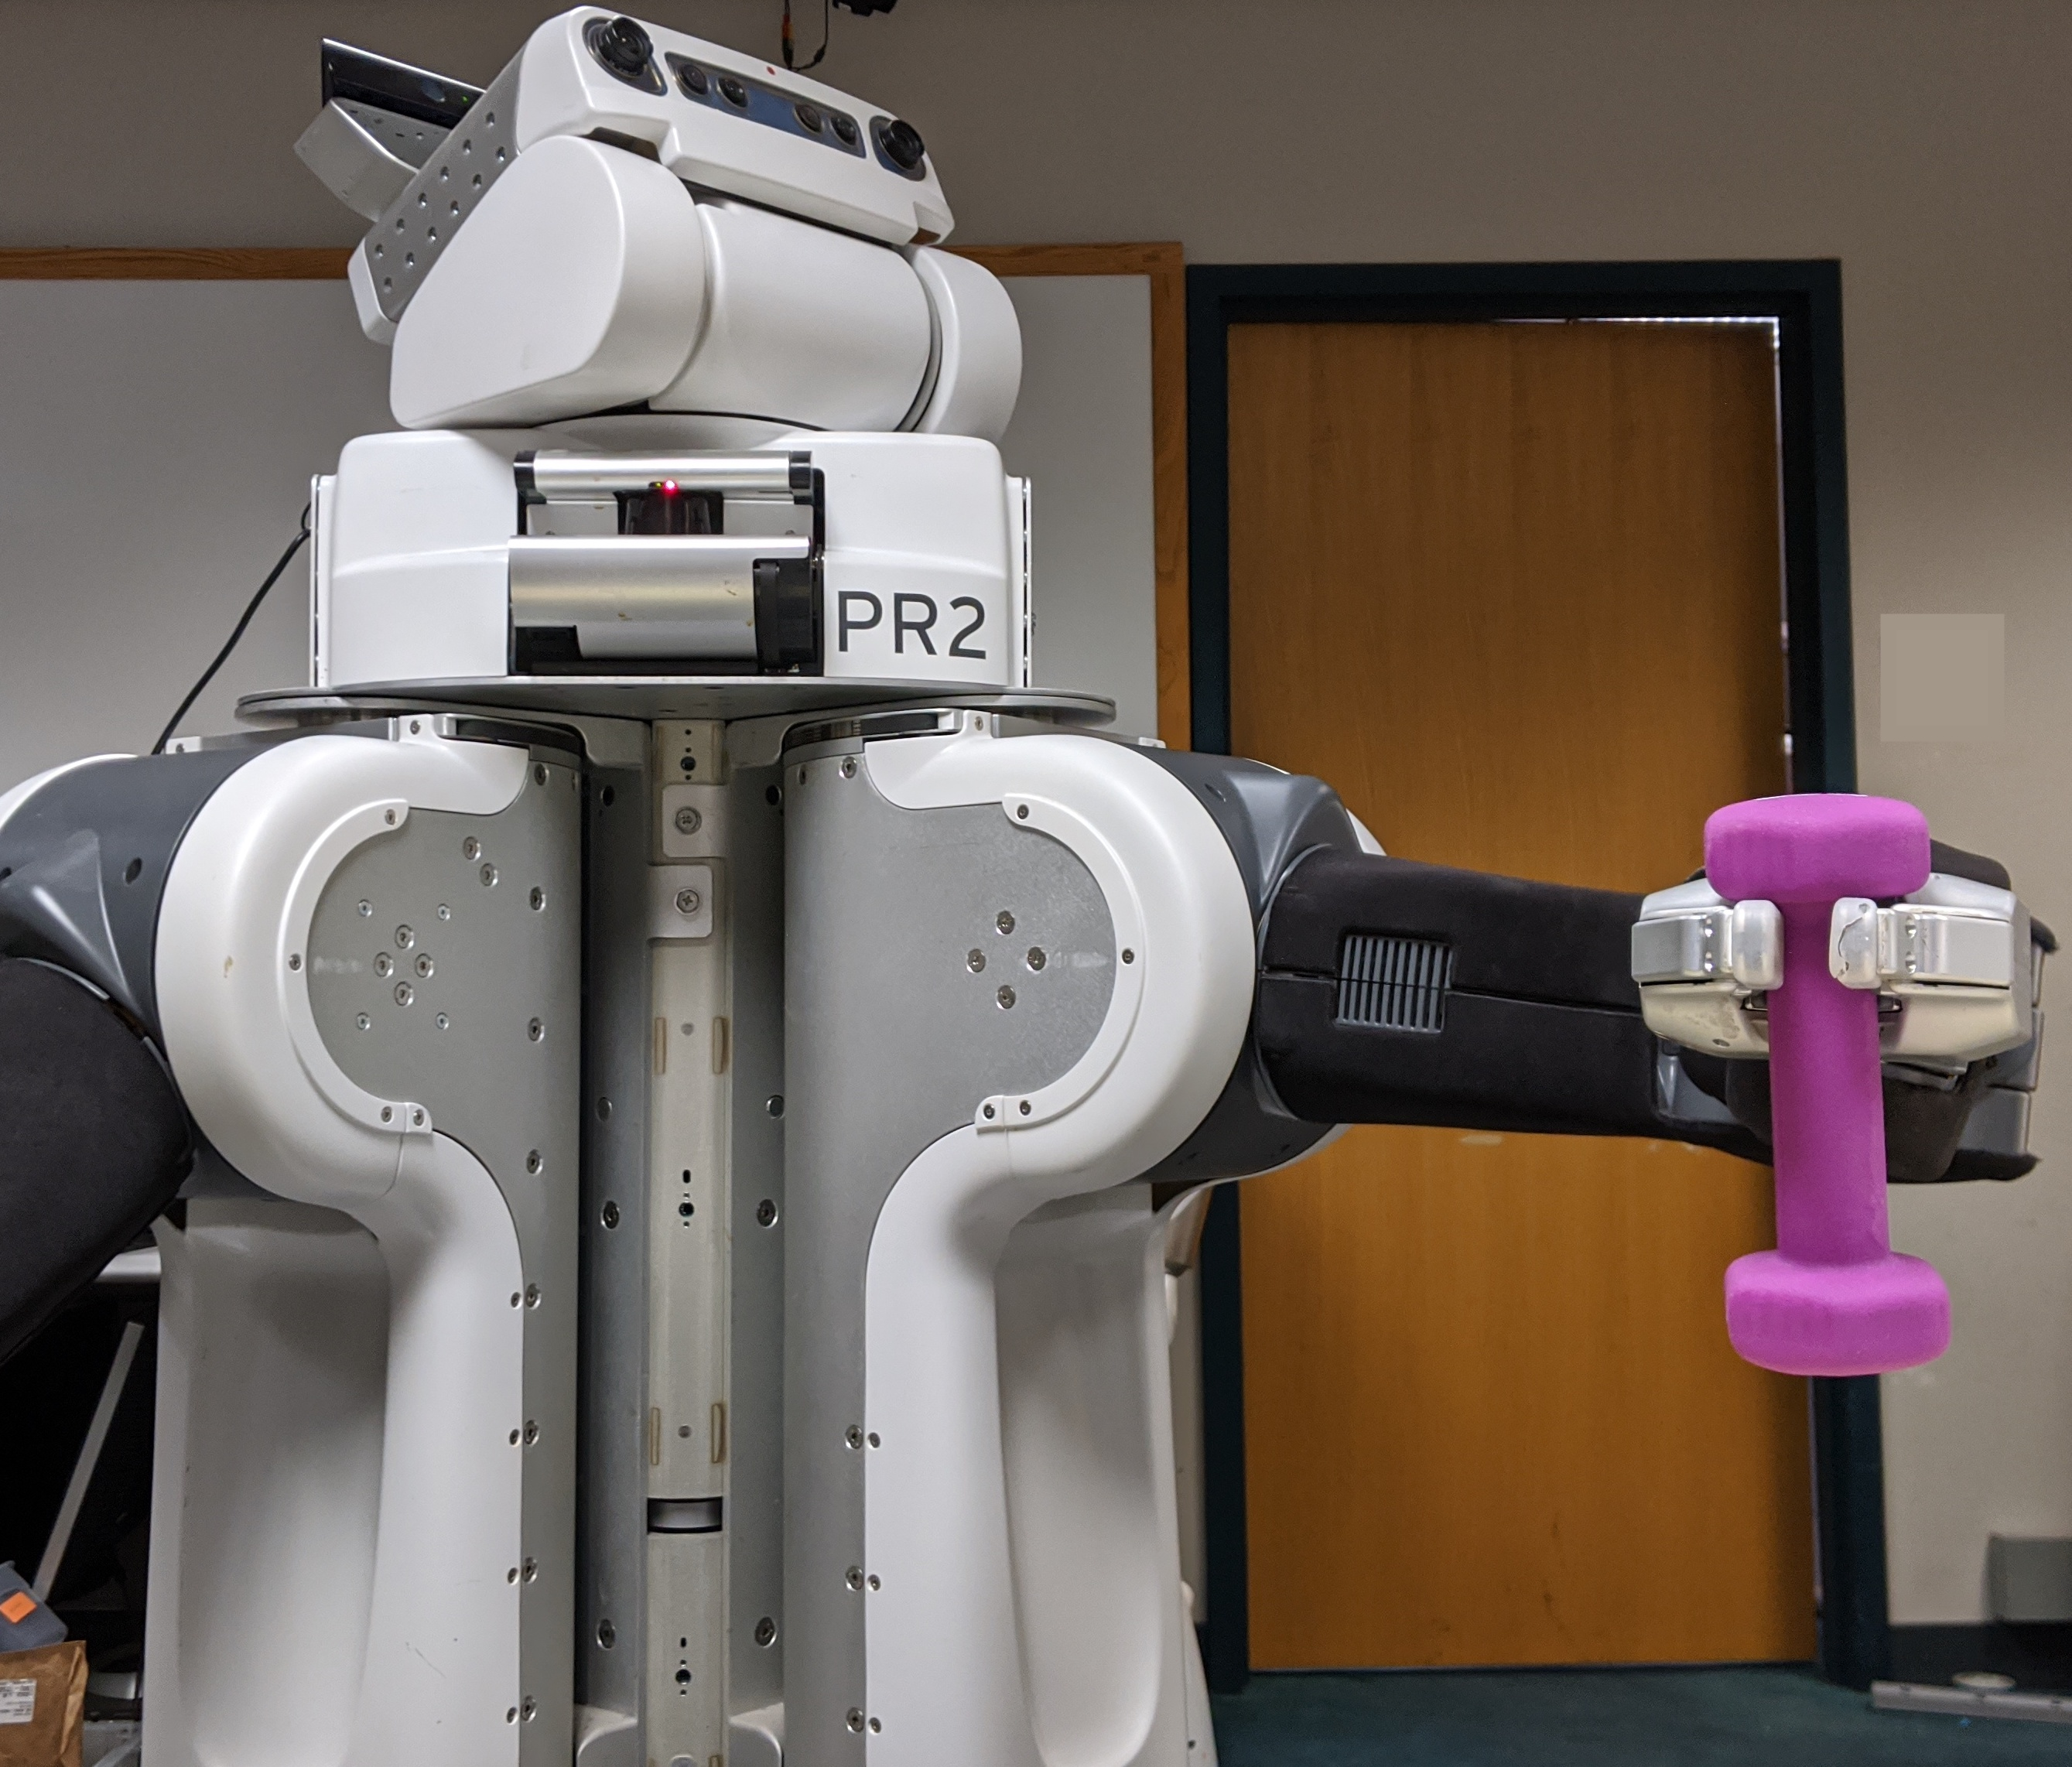
\includegraphics[width=\linewidth]{figures/cmax/pr2_dumbbell_full.jpg}
  \end{subfigure}
  %\hspace{3mm}
  \begin{subfigure}{.4\columnwidth}
    \includegraphics[width=\linewidth]{figures/cmax/gridworld_ice.pdf}
  \end{subfigure}  
  \caption{(left) PR2 executing a pick-and-place task with a heavy
    object that is modeled as light, resulting in hitting joint torque
    limits during execution. (right) Mobile
    robot navigating a gridworld with icy states, where the robot slips, that are not modeled
    as icy resulting in discrepancy in dynamics.}
  \label{fig:intro}
  
\end{figure}

For example, consider the task depicted in Figure~\ref{fig:intro}
(left) where a robotic arm needs to pick an object and place it at a
goal location. Without knowledge of the mass of the object, the model
can be inaccurate in simulating the dynamics. If the object is modeled
as light, the planned 
path would pick it to a certain height before placing it at the
goal location. However, if the object is heavy in the real world, like
in Figure~\ref{fig:intro} (left), this plan cannot be executed as the
joint torque limits are reached and the arm cannot move higher. Thus, by
using the inaccurate model for planning, the arm is stuck and cannot reach the
goal. Figure~\ref{fig:intro} (right) presents another simple scenario
where a mobile robot is navigating a gridworld containing icy
states, where the robot slips, i.e.
if the robot tries to go right or left in an icy state, it will move two cells rather
than one cell in that direction. However, the model used for planning
does not model the icy states and hence, cannot
simulate the real world dynamics correctly. This can lead to highly
suboptimal paths or sometimes even inability to reach the goal, when using such a model for planning.

A typical solution to this problem is to update the dynamics of the
model and replan \cite{DBLP:journals/sigart/Sutton91}. However, this
is often impossible in real world planning problems 
where we use models that are complex and in some cases obtained from
expensive computation that is done offline before execution
\cite{DBLP:conf/wafr/HauserBHL06}. The
dynamics of these models cannot be changed online arbitrarily without
deteriorating their simulation capabilities in other scenarios and sacrificing
real-time execution. In addition, this solution might require us to have
the knowledge of what part of the model dynamics is inaccurate and
how to correct it. Going
back to the pick-and-place example in Figure~\ref{fig:intro}, to
update the model we need to first identify
that the modeled mass is incorrect and then estimate the true mass to
correct the dynamics of the model. Both of these steps require
specialized non-trivial implementations. Finally, in the case of models that
\emph{can} be updated online efficiently, it might still not be possible to
model the true dynamics without an unreasonably large number of online
executions because the true dynamics are
often very complex, e.g. modeling cooperative navigation dynamics in
human crowds \cite{DBLP:conf/icra/VemulaMO17}. The above aspects make the 
solution of updating model dynamics online undesirable in real world robotic
tasks, where we are interested in completing the task and \emph{not} in
modeling the dynamics accurately.

In this work, we present an alternative approach \textsc{Cmax} for
interleaving planning and 
execution that does not require updating
the dynamics of the model. Instead during execution, whenever we discover an action
where the dynamics differ between the real world and the model, we
update the cost function to penalize executing such state-action pairs
in the future. This biases the planner to replan paths that do not
consist of such state-action pairs, and thereby avoid regions of
state-action space where the dynamics are known to differ. Based on
this idea, we present
algorithms for both small state spaces, where we can do
exact planning, and large state spaces, including continuous state
spaces, where we resort to function 
approximation to update the cost function and to maintain cost-to-go
estimates.
Our framework \textsc{Cmax} comes with provable guarantees on
reaching 
the goal, without any resets, under specific assumptions on
the model.
The proposed algorithms are tested on a range of tasks
including simulated 4D planar pushing as well as
physical robot 3D pick-and-place task where the mass of the object is
incorrectly modeled, and 7D arm planning tasks when one of the joints
is not operational, leading to discrepancy in dynamics. 


\section{Preliminaries}
\label{sec:preliminaries}

We are interested in the deterministic shortest path problem
represented by the tuple $M = (\statespace, \actionspace, \goalspace,
f, c)$ where $\statespace$ denotes the state space, $\actionspace$
denotes the action space, $\goalspace \subseteq \statespace$ is the
non-empty set of goal states we are
interested in reaching, $f: \statespace \times \actionspace
\rightarrow \statespace$ denotes the deterministic dynamics governing
the transition to next state given current state and action, and $c:
\statespace \times \actionspace \rightarrow [0, 1]$ is the cost
function. For the purposes of
this work, we will focus on small
discrete action spaces, bounded costs lying between $0$ and
$1$\footnote{Any bounded non-negative cost can be scaled to fit
  this assumption}, and a cost-free termination goal state i.e. for
all $g \in \goalspace$, we have
$c(g, a) = 0$
and $f(g, a) = g$ for all actions $a \in \actionspace$.
% In our
% motivating gridworld example (Figure~\ref{fig:intro} right), $\statespace$ is the $2$D discretized
% grid, $\actionspace$ consists of the $4$ actions that move the robot in
% the 4 cardinal directions by one cell, the goal space consists of the
% goal cell that we wish the agent to reach, the deterministic dynamics $f$
% simply move the robot to the next cell according to the action
% executed and whether the state is icy or not, and the cost
% is $1$ if the robot is not at goal, $0$ otherwise.
The objective of the shortest path problem is to find the least-cost path from any given start state $\startstate
\in \statespace$ to any goal state $g \in \goalspace$
in $M$.
% \begin{figure}[t]
%   \centering
%   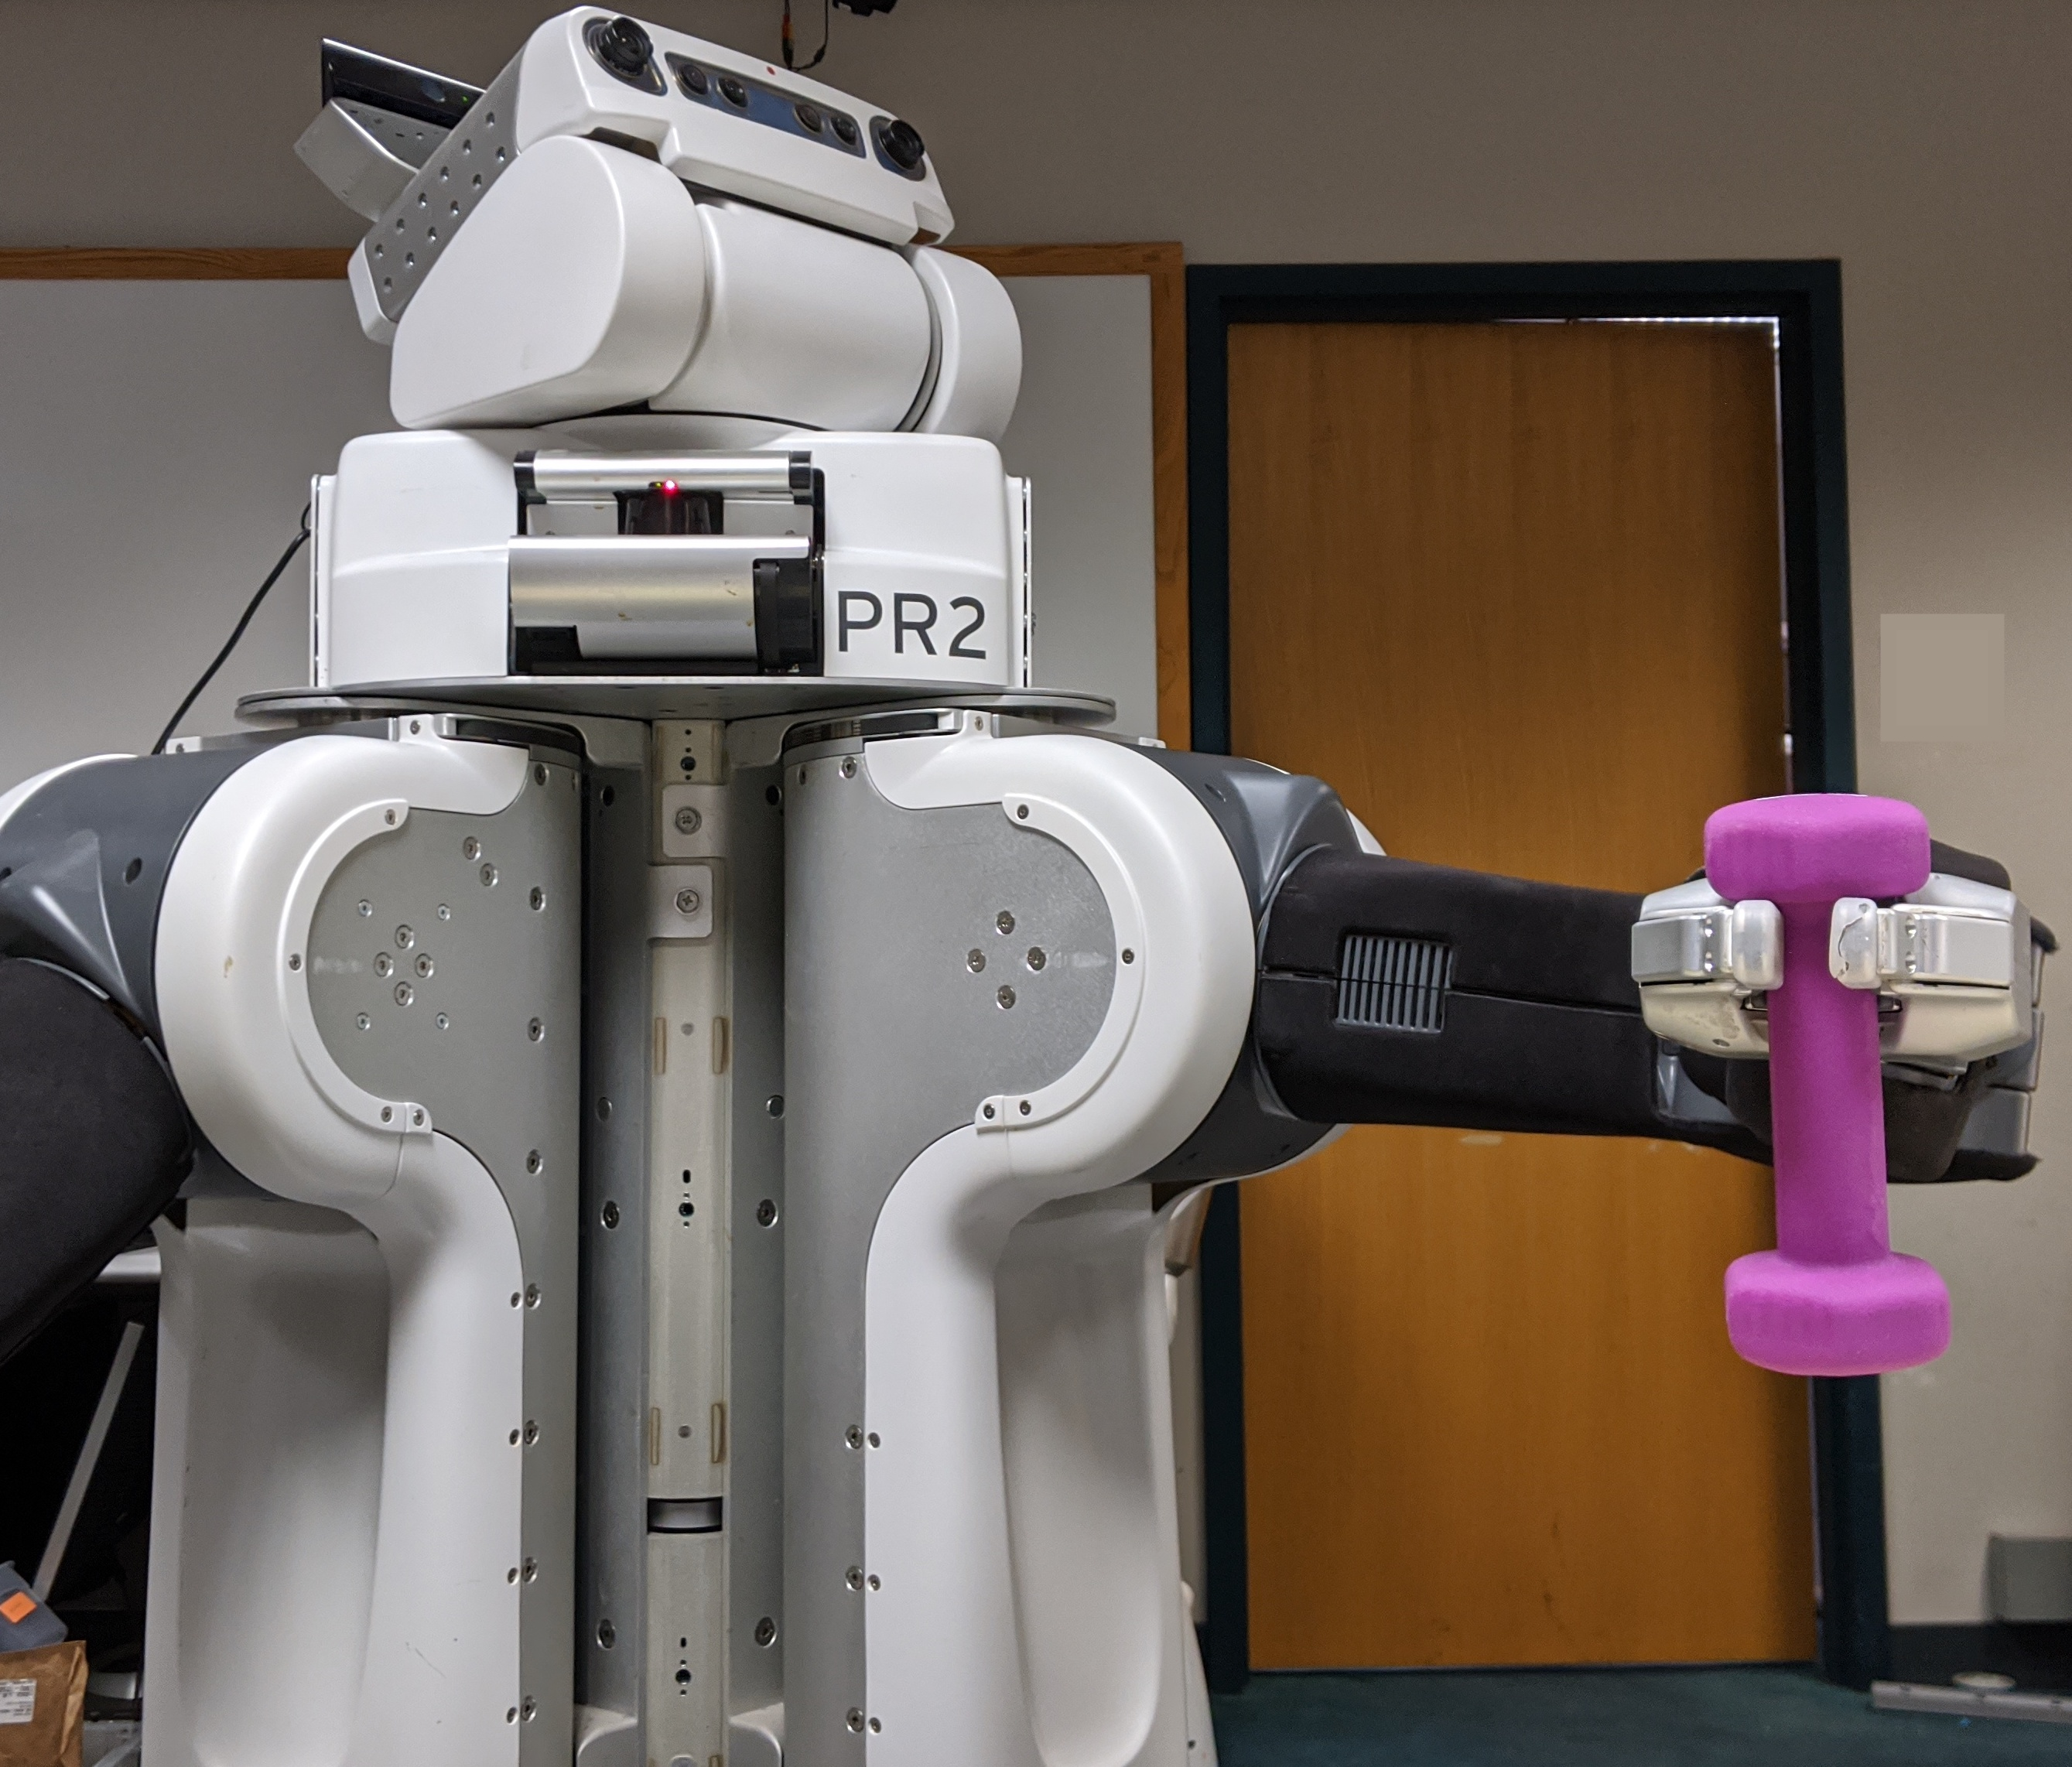
\includegraphics[width=0.6\linewidth]{figures/cmax/pr2_dumbbell_full.jpg}
%   \caption{PR2 executing a pick-and-place task with a heavy
%      object that is modeled as light, resulting in hitting joint torque
%      limits during execution.}
%    \label{fig:intro}
% \end{figure}
We assume that there
exists at least one path from each state $s \in
\statespace$ to one of the goal states $g \in \goalspace$ in $M$, and
that the
cost of any transition starting from a non-goal state is positive i.e. $c(s, a)
> 0$ for all $s \in \statespace \setminus \goalspace, a \in
\actionspace$. These assumptions are typical for analysis in
deterministic shortest path problems
\cite{DBLP:books/lib/Bertsekas05}. 
We use $V(s)$ to denote the cost-to-go estimate of any state $s \in
\statespace$ and $V^*(s)$ to denote the optimal cost-to-go. From
dynamic programming literature \cite{DBLP:books/lib/Bertsekas05}, we know
that the optimal cost-to-go satisfies the Bellman optimality condition
$V^*(s) = \min_{a \in \actionspace} [c(s, a) + V^*(f(s, a))]$.
% A stationary policy $\pi:\statespace \rightarrow 
% \actionspace$ is a deterministic rule that produces
% the action to execute at any given state, and we use $V_M^\pi(s_i) =
% \sum_{t=i}^\infty c(s_t, \pi(s_t))$ to
% denote the cost-to-go of the policy $\pi$ from state $s$. From the definition, we can
% see that any policy that does not reach goal has infinite cost-to-go
% and from our assumption, there exists at least one policy that reaches
% the goal and has finite cost-to-go. From dynamic programming
% literature \cite{bertsekas1995dynamic}, we know that among the
% policies with finite cost-to-go there exists an
% optimal stationary policy $\pi^*$ that satisfies the Bellman optimality condition
% $V_M^\optimalpolicy(s) = \min_{a \in \actionspace}c(s, a) +
% V_M^\optimalpolicy(f(s, a))$ and $V_M^{\pi^*}(s) \leq V_M^\pi(s)$, for
% all $s \in \statespace$ and any policy $\pi$.
A cost-to-go estimate $V$ is
called admissible if it underestimates the optimal cost-to-go
$V(s) \leq V^*(s)$ for all $s \in \statespace$, and
is called consistent if it satisfies the condition that for any
state-action pair $(s, a), s\notin\goalspace$, $V(s) \leq c(s, a) + V(f(s, a))$, and $V(g) = 0$ for
all $g \in \goalspace$.
% Our goal of
% finding the least-cost path from any start state to a goal state is the
% same as finding the optimal policy $\optimalpolicy$.

In this work, we assume that the exact dynamics are
initially unknown to the robot, and can only be discovered through
executions. Thus, instead of offline planning
methods, we need
online methods that interleave planning with action execution. Specifically, we 
%In this work, we specifically
focus on the online real-time planning
setting where the robot does not have access to resets, and the
robot has to interleave planning and execution to ensure real-time
operation. This is similar to the classical real-time search setting
considered by works like LRTA*~\cite{DBLP:journals/ai/Korf90},
RTAA*~\cite{DBLP:conf/atal/KoenigL06}, RTDP~\cite{DBLP:journals/ai/BartoBS95} and
several others. An important aspect of these approaches is that the robot can only perform a fixed amount of
computation for planning, independent of the size of state space, before it has to execute an action.
% This section introduces notation used throughout the
% paper. In this work, we focus on deterministic MDPs represented by the
% tuple $M = (\statespace, \actionspace, f, c)$, where $\statespace$ is the
% state space, $\actionspace$ is the action space, $f: \statespace
% \times \actionspace \rightarrow \statespace$ is the deterministic
% dynamics, and $c: \statespace \times \actionspace \rightarrow [0, 1]$
% is the cost function. $\gamma \in [0, 1)$ is the discount
% factor. For the purposes of this work, we will focus on small discrete
% action spaces, deterministic dynamics and bounded costs lying between
% $0$ and $1$\footnote{Any bounded cost function can be scaled to fit
%   this assumption}. 
% A stationary policy is a deterministic decision rule that produces an
% action based on only the current state. For any policy $\pi$, we use
% the notation $V_M^\pi(s)$ to denote the infinite-horizon discounted
% state value function and similarly use $Q_M^\pi(s, a)$ to denote the state-action
% value function. We also define a $T$-step value function for a
% positive integer $T$, $V_M^\pi(s, T)$ for any policy
% $\pi$. Specifically, $V_M^\pi(s) = \sum_{t=1}^\infty \gamma^{t-1} c_t$
% and $V_M^\pi(s, T) = \sum_{t=1}^T \gamma^{t-1}c_t$ where $c_1, c_2,
% \cdots$ are the sequence of costs incurred by following the policy $\pi$ from
% state $s$. The optimal policy is denoted using $\pi^*$ and has value
% functions $V_M^*$ and $Q_M^*$. Due to the bounded costs, the value
% function cannot be greater than $\frac{1}{1-\gamma}$. From Dynamic
% Programming literature \cite{puterman2014markov}, we know that the optimal value functions
% satisfy the Bellman optimality condition, i.e. $V_M^*(s) = \min_{a \in
% \actionspace} c(s, a) + \gamma V_M^*(f(s, a))$ for all $s \in
% \statespace$.

% We care about the sample complexity of exploration, a metric
% introduced in \cite{kakade2003sample}, which counts the number of timesteps
% $t$ in which the learning algorithm\footnote{The agent acting in the
%   MDP is guided by the learning algorithm} executes a non $\epsilon$-optimal
% policy. Observe that any learning algorithm $\algo$ that guides the
% agent to act based on its past state-action visitations is a
% non-stationary policy. Consider the agent's
% policy after we stop the algorithm at $(t-1)$ and denote it by
% $\algo_t$. This policy has a value function $V_M^{\algo_t}(s_t)$, where
% $s_t$ is the state at time-step $t$. We say the policy is
% $\epsilon$-optimal if $V^{\algo_t}_M(s_t) - V^*_M(s_t) \leq
% \epsilon$. In our online setting, the algorithm $\algo$ is run for an
% infinite-length trajectory without any resets. The sample complexity
% of exploration of $\algo$ is defined to be the number of timesteps $t$
% such that the non-stationary policy at time $t$, $\algo_t$ is not
% $\epsilon$-optimal from the current state $s_t$,
% i.e. $V^{\algo_t}_M(s_t) > V^*_M(s_t) + \epsilon$. This definition
% captures the efficiency of the algorithm in dealing with the
% exploration-exploitation dilemma during online execution.

\section{Problem Setup}
\label{sec:problem-setup}

Consider the problem of a robot acting to find a least-cost path to a
goal in an environment represented
by the tuple $M = (\statespace, \actionspace, \goalspace, f, c)$ with unknown
deterministic dynamics $f$ and known cost function $c$. The robot
gathers knowledge of the dynamics over a single
trajectory in the environment, and does not have access to any
resets, ruling out any episodic approach.
This is an extremely challenging setting as the robot has to reason
about whether to exploit its current knowledge of the dynamics to act
near-optimally or to explore to gain more knowledge of the dynamics,
possibly at the expense of suboptimality.

We assume that the agent has access to an approximate model, $\hat{M} = (\statespace,
\actionspace, \goalspace, \hat{f}, c)$, that it can use to simulate the outcome of
its actions and use for planning. In our motivating gridworld example
(Figure~\ref{fig:intro} right), this model
represents a grid with no icy states, so the dynamics $\hat{f}$
moves the robot to the next cell based on the executed
action without any slip. However, the real environment contains
icy states
resulting in dynamics $f$ that differ on state-action pairs where the
state is icy. For the remainder of this paper, we will
refer to such state-action pairs where $f$ and $\hat{f}$ differ as ``incorrect''
state-action pairs, and 
%Note that the dynamics of the simulator $\hat{f}$ is a
%good approximation of the environment dynamics $f$, but not
%everywhere.
use the notation $\incorrectset \subseteq
\statespace \times \actionspace$ to denote the set of ``incorrect'' state-action
pairs,
i.e. $f(s, a) \neq \hat{f}(s, a)$ for all $(s, a) \in
\incorrectset$.
% It is important to note that we do not have any
% knowledge of the set $\incorrectset^*$ ahead of online execution. 
The objective is for the robot to reach a goal
state from a given start state, despite using an inaccurate model for planning, while
minimizing the cost incurred and ensuring real-time execution.

% The intuition is that if the model $\hat{M}$ is a very good
% approximation of the environment $M$, then we expect
% % a policy obtained
% % from planning in the simulator to act near-optimally in the
% % environment during online execution. 
% the robot to reach a goal in the environment $M$ during online
% execution, despite using the model $\hat{M}$ for planning.
% However, in most realistic
% scenarios, it is rare to have a model that approximates environment dynamics very
% well.
% , and it is a significant challenge to
% ensure that the robot reaches a goal in the environment with
% differing dynamics. 

\section{Approach}
\label{sec:approach-1}

Existing planning and learning approaches try to learn a very good
approximation of $M$ from scratch 
through online executions \cite{DBLP:journals/ml/KearnsS02, DBLP:journals/jmlr/BrafmanT02, DBLP:conf/atal/JongS07,
  DBLP:journals/pami/DeisenrothFR15}, or update the dynamics of model
$\hat{M}$ so that it approximates $M$ well \cite{DBLP:conf/icml/AbbeelQN06,
  DBLP:conf/aaai/Jiang18, rastogi2018sample}.
% In this work, we take a
% different approach. Our main motivation is
% that modern planning approaches
% use forward models that are complex and in some cases, obtained from expensive
% computation that is done offline. For example, motion planning usually
% involves using analytical motion primitives \cite{DBLP:conf/icra/CohenCL10} that are precomputed offline and
% are difficult to update during online execution without sacrificing
% real-time capabilities.
% The dynamics
% of these forward models cannot be changed online in any arbitrary way without
% deteriorating their performance in other scenarios and sacrificing
% real-time capabilities. In addition, to update the model dynamics we
% might require knowledge about the environment that we are uncertain
% about, like the mass of the object in our pick-and-place example in
% Figure~\ref{fig:intro} (left), which is hard to obtain.
% In domains where we do have models that can be updated
% efficiently online it might not be possible to model the true
% dynamics as it can be extremely complex and could potentially take a
% large number
% of real world executions to learn a reasonable approximation.
In this work, we propose an approach \textsc{Cmax} that uses
the inaccurate model $\hat{M}$ online \emph{without} updating its dynamics, and
is provably guaranteed to complete the task.
% Most robotic simulations
% are sophisticated, based on physics and have complex optimization
% procedures to resolve contacts \cite{todorov2012mujoco}. Such
% simulator dynamics cannot be changed in any arbitrary way without
% deteriorating performance in other scenarios. Thus, we treat them as
% black-boxes whose dynamics cannot be manipulated. A similar problem
% was tackled in \cite{jiang2018pac} in the episodic
% setting\footnote{Unlike the online setting, the agent experiences the
%   MDP in episodes.} for small
% state spaces. We will tackle it in the online setting considering both
% small and large state spaces.
In a nutshell, instead of learning a new dynamics model from scratch or
updating the dynamics of existing model,
% our approach
\textsc{Cmax}
maintains a
running estimate of the set $\incorrectset_t$ consisting of all
state-action pairs that have been executed and have been discovered to
be incorrect until timestep $t$. Using the set $\incorrectset_t$, we update the cost
function to bias the planner to plan future paths that avoid
state-action pairs that are known to be incorrect.
% This
% ensures that the cost-to-go estimates obtained from planning in the
% model are trustworthy, and the robot does not waste time and
% computation in planning and executing state-action pairs that are known to
% be incorrect.
It is
important to note that the challenge of dealing with
exploration-exploitation dilemma online still exists, as we do not
know the set of state-action pairs $\incorrectset$ where the dynamics differ ahead of online
execution. A similar approach was proposed in \cite{DBLP:conf/aaai/Jiang18} for the
episodic setting where the robot had access to resets, and for small
state spaces where we could perform full state space planning.
% Our approach
\textsc{Cmax}
extends it to the significantly more challenging 
online real-time setting and we present a practical algorithm for
large state spaces. 

\subsection{Penalized Model}
\label{sec:penalized-model}

We formalize
our approach
as follows: Given a model
$\approximateMDP$ and a set $\incorrectset \subseteq \statespace
\times \actionspace$ consisting of state-action pairs that have been
discovered to be incorrect so far, define the penalized model $\penalizedMDP_\incorrectset$ as:
\begin{definition}[Penalized Model]
  The penalized model $\penalizedMDP_\incorrectset = (\statespace,
  \actionspace, \goalspace,
  \hat{f}, \tilde{c}_\incorrectset)$ has the same state space,
  action space, set of goals, and dynamics as $\approximateMDP$. The
  cost function $\tilde{c}_\incorrectset$ though
  is defined as $\tilde{c}_\incorrectset(s, a) = |\statespace|$ if $(s, a) \in
  \incorrectset$, else $\tilde{c}_\incorrectset(s, a) =
  c(s,a)$.\footnote{This is similar to the notion of penalized MDP,
    introduced in \cite{DBLP:conf/aaai/Jiang18}}
  % \begin{equation}
  %   \label{eq:1}
  %   \tilde{c}_\incorrectset(s, a) =
  %   \begin{cases}
  %     |\statespace| & (s, a) \in \incorrectset \\
  %     c(s, a) & \mathsf{otherwise}
  %   \end{cases}
  % \end{equation}
  % where $\vmax$ is a large value corresponding to the maximum
  % cost-to-go of any policy that is guaranteed to reach the goal.
  \label{def:penalized-mdp}
\end{definition}

Intuitively, the penalized model $\penalizedMDP_{\incorrectset}$
has a very high cost for any transition where the dynamics differ,
i.e. $(s, a) \in \incorrectset$, and
the same cost as the model $\hat{M}$ otherwise. More specifically, the
cost is inflated to the size of the statespace, which is the maximum
cost of a path that visits all states\footnote{Hence, the name \textsc{Cmax} for our approach} (remember, that our cost is
normalized to lie within $0$ and $1$.) This biases the planner to ``explore'' all other
state-action pairs that are not yet known to be incorrect before it
plans a path through an incorrect state-action pair.
% Note that the
% penalized model $\penalizedMDP_\incorrectset$ has the same dynamics as
% the initial model $\hat{M}$.
% Thus, by using the
% penalized model $\penalizedMDP_\incorrectset$ for planning the robot's
% next action we force the planner to
% plan paths that traverse state-action space where the model $\hat{M}$ is
% a good approximation of the environment $M$.
In the next section, we
will describe how we use the penalized model
$\penalizedMDP_\incorrectset$ for real-time planning.
%A similar notion of penalization is defined in
%\cite{jiang2018pac} but having a different dynamics compared to the
%simulator by terminating at any $(s, a) \in \incorrectset^*$. But we
%cannot employ that definition in the online setting as we
%experience the MDP in a single trajectory.

% Our setting where the dynamics of the model $\hat{M}$ cannot be
% modified can be simply thought of as the agent acting in the penalized
% model $\penalizedMDP_{\incorrectset^*}$. However, we do not know
% $\incorrectset^*$ before execution so the agent needs to reason about
% exploration-exploitation. To assess the efficiency of our approach, we
% will use the same performance metric defined in Section
% \ref{sec:preliminaries} but with respect to the optimal policy in
% $\penalizedMDP_{\incorrectset^*}$ rather than the environment $M$,
% i.e. sample complexity of exploration is the number of timesteps $t$
% where $V_{\penalizedMDP_{\incorrectset^*}}^{\algo_t}(s_t) >
% V_{\penalizedMDP_{\incorrectset^*}}^*(s_t) + \epsilon$. Note that this is
% still a very useful metric to measure the efficiency of our learning
% algorithm, especially in the case where the simulator $\hat{M}$ is a
% good approximation of the environment in large regions of state-action
% space, i.e. $|\incorrectset^*|$ is small. In other words, we can only
% hope to perform as optimally as the optimal policy for the penalized
% MDP $\penalizedMDP_{\incorrectset^*}$. We will discuss more on this in
% Section \ref{sec:discussion}.

\subsection{Limited-Expansion Search for Planning}
\label{sec:limit-expans-search}

During online execution, the robot has to constantly plan the next
action to execute from its current state in real-time. This forces the
robot to use a fixed amount of computation for planning before it has
to execute the best action found so far. In this work, we use
a real-time search method that is adapted from RTAA*
proposed by \cite{DBLP:conf/atal/KoenigL06}.

\begin{algorithm}[t]
  \caption{Limited-Expansion Search based on
    RTAA*\cite{DBLP:conf/atal/KoenigL06}}
  {\normalsize
  \begin{algorithmic}[1]
    \Function{$\mathtt{SEARCH}$}{$s,
      \penalizedMDP_{\incorrectset}, V, K$}
    \State Initialize $g(s) \leftarrow 0$
    \State Initialize min-priority open list $O$, and closed list $C$
    \State Add $s$ to open list $O$ with priority $g(s) + V(s)$
    \For{$i=1, 2, \cdots, K$}
    \State Pop $s_i$ from open list $O$
    \State If $s_i \in \goalspace$, then $s_{\mathsf{best}} \leftarrow
    s_i$ and move to Line~\ref{line:updates}
    \For{$a \in \actionspace$} \Comment{\textit{Expanding state $s_i$}}
    \State Get successor $s' = \hat{f}(s_i, a)$
    \State If $s' \in C$, continue to next action
    \If{$s' \in O$ and $g(s') > g(s_i) + \tilde{c}_\incorrectset(s_i, a)$}
    \State Update $g(s') \leftarrow g(s_i) + \tilde{c}_\incorrectset(s_i,
    a)$
    \State Reorder open list $O$
    \ElsIf{$s' \notin O$}
    \State Set $g(s') \leftarrow g(s_i) + \tilde{c}_\incorrectset(s_i, a)$
    \State Add $s'$ to $O$ with priority $g(s') + V(s')$
    \EndIf
    \EndFor
    \State Add $s_i$ to the closed list $C$
    \EndFor
    \State Pop $s_{\mathsf{best}}$ from open list
    $O$\label{line:pop-best-node}
    \For{$s' \in C$}\label{line:updates}
    \State Update $V(s') \leftarrow
    g(s_{\mathsf{best}}) + V(s_{\mathsf{best}}) - g(s')$\label{line:cost-to-go-update}
    \EndFor
    \State Backtrack from $s_{\mathsf{best}}$ to $s$, and set
    $a_{\mathsf{best}}$ as the first action on path from $s$ to
    $s_{\mathsf{best}}$
    
    \Return{$a_{\mathsf{best}}$}
    \EndFunction
  \end{algorithmic}}
  \label{alg:limited-expansion-search}
\end{algorithm}

The planner is summarized in Algorithm~\ref{alg:limited-expansion-search}. At any
timestep $t$, given the
current penalized model $\penalizedMDP_{\incorrectset_t}$ and the current
state $s_t$, the planner constructs a lookahead
search tree using at most $K$ state expansions. We obtain the successors of any
expanded state and the cost of any state-action pair using the
penalized model $\penalizedMDP_{\incorrectset_t}$.
After expanding $K$
states, it finds the best state $s_{\mathsf{best}}$ among the leaves of the search tree
that has the least sum of cost-to-come from $s_t$ and
cost-to-go to a goal state (line~\ref{line:pop-best-node} in Algorithm~\ref{alg:limited-expansion-search}). The best action to execute in the current
state $s_t$ is chosen to be the first action on the path from $s_t$ to
$s_{\mathsf{best}}$ in the search tree and the cost-to-go estimates of
all expanded states are updated as: $V(s_{\mathsf{expanded}}) =
g(s_{\mathsf{best}}) + V(s_{\mathsf{best}}) -
g(s_{\mathsf{expanded}})$, where $g(s)$ is the cost-to-come from $s_t$
for any state $s$ in the search tree.
The amount of computation used to compute the best action for the
current state is bounded as a factor of the number of expansions $K$ in the search
tree. Thus, we can bound the planning time and ensure real-time
operation for our robot.

% Before presenting an algorithm for planning and execution using
% inaccurate models for large state spaces in Section~\ref{sec:large-state-spaces}, we will first
% present an algorithm for small discrete state spaces in the next
% section.
% Before presenting our algorithm for planning and execution using
% inaccurate models, we describe the assumptions that we need
% to establish provable guarantees of our approach in the next section.

% \subsection{Assumptions}
% \label{sec:assumptions}

\subsection{Warm Up: Small State Spaces}
\label{sec:small-state-spaces}

In this section, we will present an algorithm that is applicable for
small discrete state spaces where it is feasible to maintain cost-to-go
estimates for all states $s \in \statespace$ using a tabular representation, and we can maintain a
running set $\incorrectset_t$ containing all the discovered incorrect state-action pairs
so far, without resorting to function approximation. The algorithm\footnote{A similar algorithm in the
  episodic setting with full state space planning is presented in \cite{DBLP:conf/aaai/Jiang18}} is shown in Algorithm
\ref{alg:small-state-spaces}.
Intuitively, Algorithm \ref{alg:small-state-spaces} maintains a
running set of incorrect state-action pairs
$\incorrectset_t$, updates the set whenever it encounters an incorrect
state-action pair, and recomputes the penalized model
$\penalizedMDP_{\incorrectset_t}$. Crucially, the algorithm never updates the
dynamics of the model $\approximateMDP$, and only updates the cost
function according to Definition~\ref{def:penalized-mdp}.
In order to prove completeness, we assume the following:
\begin{assumption}
  Given a penalized model $\tilde{M}_{\incorrectset_t}$ and the current
  state $s_t$ at any timestep $t$, there always exists at least one path from $s_t$ to a goal
  state that \textit{does not contain} any state-action pairs $(s, a)$ that are known to
  be incorrect, i.e. $(s, a) \in \incorrectset_t$. \footnote{This
    assumption is less restrictive than the assumption that
    there exists at least one path from the current state to a goal
    that does not contain any state-action pairs $(s, a)$ that are incorrect i.e. $(s,
    a) \in \incorrectset$}
  \label{assumption:core}
\end{assumption}

\begin{algorithm}[t]
  \caption{\textsc{Cmax} -- Small State Spaces}
  {\normalsize
  \begin{algorithmic}[1]
    \State Initialize $\approximateMDP_1 \leftarrow \approximateMDP$,
    $\incorrectset_1 \leftarrow \{\}$, start state $s_1 \in
    \statespace$, cost-to-go estimates $V$, number of expansions $K$,
    $t \leftarrow 1$
    \While{$s_t \notin \goalspace$}
    \State Get $a_t = \mathtt{SEARCH}(s_t, \hat{M}_t, V, K)$
    \State Execute $a_t$ in environment $M$ to get $s_{t+1} = f(s_t, a_t)$
    \If{$s_{t+1} \neq \hat{f}(s_t, a_t)$}
    \State Add $(s_t, a_t)$ to the set : $\incorrectset_{t+1} \leftarrow \incorrectset_t \cup
    \{(s_t, a_t)\}$
    \State Update the penalized model : $\approximateMDP_{t+1} \leftarrow
    \penalizedMDP_{\incorrectset_{t+1}}$
    \Else
    \State $\incorrectset_{t+1} \leftarrow \incorrectset_t$,
    $\approximateMDP_{t+1} \leftarrow \approximateMDP_t$
    \EndIf
    \State $t \leftarrow t + 1$
    \EndWhile
  \end{algorithmic}}
  \label{alg:small-state-spaces}
\end{algorithm}

% Observe that this assumption is on both the quality of the initial
% model $\hat{M}$ and the operation of our algorithm.
% We would like to emphasize that this assumption
% is less restrictive than the following assumption:
% \begin{assumption}
%   For any state $s \in \statespace$, there always exists at least one
%   path from $s$ to a goal state that \textit{does not contain} any
%   incorrect state-action pairs, i.e. $(s, a) \in \incorrectset^*$.
%   \label{assumption:strong}
% \end{assumption}

% It is easy to see that Assumption~\ref{assumption:strong}
% implies Assumption~\ref{assumption:core} since for any timestep $t$,
% $\incorrectset_t \subseteq \incorrectset^*$. We will show that
% Assumption~\ref{assumption:core} does not imply
% Assumption~\ref{assumption:strong} through an example: Recall the
% motivating icy gridworld from Figure~\ref{fig:intro} and consider the
% small icy gridworld shown in Figure~\ref{fig:search}
% (right). Assumption~\ref{assumption:strong} is clearly violated since
% there exists no path from robot's current state to the goal that does
% not contain any incorrect state-action pair. However,
% Assumption~\ref{assumption:core} is not violated since the action of
% moving right in the robot's current state is not yet discovered to be
% incorrect. In fact, once it executes the move right action it
% immediately reaches the goal state since the robot slips on ice and
% moves two cells to the right. Thus, Assumption~\ref{assumption:core}
% does not imply Assumption~\ref{assumption:strong}.

% To establish
% guarantees on completeness and performance of our algorithm, we will
% use the less restrictive Assumption~\ref{assumption:core}.

Under this assumption, we can show
the following guarantee for
Algorithm \ref{alg:small-state-spaces}:
\begin{theorem}
  Assume Assumption~\ref{assumption:core} holds then, if $\incorrectset$ denotes
  the set consisting of all incorrect state-action
  pairs, and the initial cost-to-go estimates used are
  admissible and consistent, then using Algorithm~\ref{alg:small-state-spaces}
  the robot is guaranteed to reach a goal state in at most
  $|\statespace|^2$ timesteps. Furthermore, if we allow for $K =
  |\statespace|$ expansions, then we can guarantee that the
  robot will reach a goal state
  in at most $|\statespace|(|\incorrectset|+1)$ timesteps.
  \label{thm:small-state-spaces}
\end{theorem}
\begin{proof}[Proof Sketch]
  From \cite{DBLP:conf/atal/KoenigL06} Theorem 3 and
Assumption~\ref{assumption:core}, we have that using
RTAA*, the robot is guaranteed to reach a goal state. Combining this
result with the $|\statespace|^2$ upper bound on the number of timesteps it takes for LRTA*
(which is equivalent to RTAA* with $K=1$ expansion) to reach the goal
from \cite{DBLP:conf/aaai/KoenigS93}, we have that using Algorithm~\ref{alg:small-state-spaces} a
robot is guaranteed to reach a goal state in at most $|\statespace|^2$
timesteps.

To prove the second part, observe that when we do $K = |\statespace|$
expansions at any timestep $t$ in RTAA* and update the cost-to-go, we obtain the optimal
cost-to-go $V^*$ for the penalized model
$\tilde{M}_{\incorrectset_t}$. Once we obtain the optimal cost-to-go,
there will be no further cost-to-go updates in subsequent timesteps
until we either discover an incorrect state-action pair or reach the
goal. Since the number of incorrect $(s, a)$ pairs is
$|\incorrectset|$ and the length of the longest path is bounded
above by $|\statespace|$, using pigeon hole principle we have
that the robot is guaranteed to reach the goal in at most
$|\statespace|(|\incorrectset| + 1)$ timesteps.
\end{proof}
% \begin{proof}
%   Proof given in Appendix \ref{sec:proof-theor-refthm:s}.
% \end{proof}
% Proof of the above theorem is given in Appendix
% \ref{sec:proof-theor-refthm:s}.
The above
theorem establishes that using Algorithm 
\ref{alg:small-state-spaces}, the robot is guaranteed to reach a goal
state under Assumption~\ref{assumption:core}. In
practice, we observe that the number of timesteps to reach a goal has a smaller
dependence on the size of state space than the
worst-case bound, especially if Algorithm~\ref{alg:small-state-spaces}
starts with cost-to-go estimates that are reasonably accurate for the
initial model $\hat{M}$. % Similar
% sample bounds for deterministic
% shortest path problems when a model is learned from scratch are shown in
% \cite{Koenig1993} and \cite{kakade2003sample}.

\subsection{Large State Spaces}
\label{sec:large-state-spaces}

In large state spaces, it is infeasible to
maintain cost-to-go estimates for all states $s \in \statespace$ using
a tabular representation and maintain a running estimate of the set
$\incorrectset_t$, as both
could be very large in size. Thus,
we will need to resort to function approximations for both
cost-to-go estimates and the set $\incorrectset_t$.

We will assume existence of a fixed distance metric $d:
\statespace \times \statespace \rightarrow \mathbb{R}^+\cup\{0\}$, and that
$\statespace$ is bounded under this metric.
% , i.e. there exists a constant
% $\deltamax$ such that for all $s, s' \in \statespace$, $d(s, s') \leq
% \deltamax$.
% In large state spaces, there could potentially be a
% large number of state-action pairs where the dynamics differ between
% the model and the real world.
We relax the definition of $\incorrectset$ using the distance
metric $d$ as follows: Define any state-action pair $(s, a) \in
\incorrectset^\xi$ to be $\xi$-incorrect if $d(f(s, a), \hat{f}(s, a))
> \xi$ where $\xi \geq  0$. We assume that there is an underlying
path following controller that is used to execute our plan and can deal with
discrepancies smaller than $\xi$. Thus, we allow for small
discrepancies in our approximate model $\hat{M}$ that can be resolved
using a low-level controller.

% To show that our function approximations can generalize, we need some
% continuity assumptions.
% We assume that the cost function $c$ satisfies
% lipschitz continuity, i.e. there exists a constant $\alpha \in \reals$,
% $\alpha \geq 0$ such that for all $a \in \actionspace$ and $s, s' \in \statespace$ we have, $|c(s, a) - c(s',
% a)| \leq \alpha d(s, s')$. We also assume lipschitz continuity in the difference of dynamics
% between model $\approximateMDP$, and environment $M$ as follows:
% $|d(f(s, a), \hat{f}(s, a)) - d(f(s', a), \hat{f}(s', a))| \leq \beta
% d(s, s')$ for all $s, s' \in \statespace$ and $a \in \actionspace$,
% where $\beta \in \reals$ and $\beta \geq 0$.
% \anirudh{Do we need any Lipschitz assumptions on the cost function or
%   dynamics or difference in dynamics?}

% . Thus, we can
% use definition \ref{def:penalized-mdp} with the set
% $\incorrectset^\xi$ to define the penalized MDP
% $\penalizedMDP_{\incorrectset^\xi}$.
% To understand why this notion
% captures the accuracy of the model $\approximateMDP$ in modeling
% the environment $M$ to find the shortest path, we can show the following lemma which is a direct
% extension of the simulation lemma from \cite{Kearns2002},
% \begin{lemma}[Simulation Lemma]
%   If the model $\approximateMDP$ satisfies the condition $d(f(s,
%   a), \hat{f}(s, a)) \leq \xi$ for all $(s, a) \in \statespace \times
%   \actionspace$, then
%   \begin{equation}
%     \label{eq:5}
%     V_{M}^*(s) \leq
%     \alpha\xi\deltamax + V_{\approximateMDP}^*(s)
%   \end{equation}
%   for any policy $s \in \statespace$.
% \end{lemma}

% Thus, planning in a model where the discrepancy in dynamics is
% bounded, i.e. $d(f(s, a), \hat{f}(s, a)) \leq \xi $, results in a path
% that is sub-optimal in a bounded fashion as given by
% Equation~\ref{eq:5}. We will use this property to bound the
% performance of our algorithm by appropriately maintaining a running
% approximation of the incorrect set $\incorrectset_t^\xi$, and updating
% the cost function according to Definition~\ref{def:penalized-mdp}.

Our algorithm for  large state
spaces is presented in Algorithm \ref{alg:large-state-spaces}. The main idea
of the algorithm is to ``cover'' the set $\incorrectset^\xi$ using
hyperspheres in $\statespace\times\actionspace$. Since the action
space $\actionspace$ is a discrete set, we maintain separate sets of
hyperspheres for each action $a \in \actionspace$. Whenever the agent encounters an incorrect
state-action pair $(s, a) \in \incorrectset^\xi$, it places a
hypersphere at $s$ corresponding to action $a$ whose radius (as
measured by the metric $d$) is given
by $\delta > 0$, a domain-dependent constant.
% This radius is obtained by using the lipschitz continuity assumption
% on the difference of dynamics, and ensures that any state $s'$ lying inside the
% hypersphere centered at $s$ corresponding to action $a$ satisfies
% either the condition $(s', a) \in \incorrectset^\xi$ or it is within a
% distance of $\delta$ from an incorrect state-action pair.
We inflate the cost of a
state-action pair $(s, a)$, according to
Definition~\ref{def:penalized-mdp},
if $s$ lies inside any hypersphere corresponding to action $a$. In
practice, this
is implemented by constructing 
separate KD-Trees in state space $\statespace$ for each action
$a \in \actionspace$ to enable efficient lookup.

After executing the action and placing a hypersphere if a discrepancy
in dynamics
was observed, the function approximation for cost-to-go is updated
iteratively as follows (Line~\ref{line:iteration-start} to
Line~\ref{line:iteration-end}): Sample a batch of states from the buffer
of previously visited states with replacement, construct a lookahead
tree for each state in the batch (through parallel jobs) to obtain all
states on the closed list and their corresponding cost-to-go updates
using Algorithm~\ref{alg:limited-expansion-search},
and finally update the parameters of the cost-to-go function
approximator to minimize the mean squared loss $\mathcal{L}(V_\theta, \mathbb{X}) = \frac{1}{2|\mathbb{X}|} \sum_{(s,
    V(s)) \in \mathbb{X}} (V(s) - V_\theta(s))^2$ for all the expanded
states through a gradient descent step (Line~\ref{line:iteration-end}).
% \begin{equation}
%   \label{eq:2}
%   \mathcal{L}(V_\theta, \mathbb{X}) = \frac{1}{2|\mathbb{X}|} \sum_{(s,
%     V(s)) \in \mathbb{X}} (V(s) - V_\theta(s))^2
% \end{equation}

Observe that, similar to Algorithm~\ref{alg:small-state-spaces}, we
do not update the dynamics $\hat{f}$ of the model, and only update the
cost function according to
Definition~\ref{def:penalized-mdp}. However, unlike
Algorithm~\ref{alg:small-state-spaces}, we do not explicitly maintain
a set of incorrect state-action pairs but maintain it implictly
through hyperspheres. By using hyperspheres, we obtain local
generalization and increase the cost of all the state-action pairs
inside a hypersphere.
% We will also show that using hyperspheres speeds
% up our approach as it quickly ``covers'' the $\xi$-incorrect
% state-action region $\incorrectset^\xi$.
In addition, unlike
Algorithm~\ref{alg:small-state-spaces}, we update cost-to-go estimates
of not only the expanded states in the lookahead tree obtained from
current state $s_t$, but also from previously visited states. This
ensures that the function approximation used for maintaining
cost-to-go estimates does not deteriorate for states that were
previously visited, and potentially help in generalization.
\begin{algorithm}[t]
  \caption{\textsc{Cmax} -- Large State Spaces}
  {\normalsize
  \begin{algorithmic}[1]
    \State Initialize $\approximateMDP_1 \leftarrow \approximateMDP$,
    Cost-to-go function approximation $V_{\theta_1}$, Set of
    hyperspheres $\incorrectset^\xi_1 \leftarrow \{\}$, Start state
    $s_1$, Number of planning updates $N$, Batch size $B$, Buffer
    $\buffer$, Number of expansions $K$,
    Learning rate $\eta$, $t \leftarrow 1$, Radius of hypersphere
    $\delta$, Discrepancy threshold $\xi$
    \While{$s_t \notin \goalspace$}
    \State Get $a_t \leftarrow \mathtt{SEARCH}(s_t, \approximateMDP_t,
    V_{\theta_{t}}, K)$
    \State Execute $a_t$ in environment $M$ to get $s_{t+1} \leftarrow
    f(s_t, a_t)$
    \If{$d(s_{t+1}, \hat{f}(s_t, a_t)) > \xi$}
    \State Add $\incorrectset_{t+1}^\xi \leftarrow
    \incorrectset_t^\xi \cup \{\mathsf{sphere}(s_t, a_t, \delta)\}$
    \Else
    \State $\incorrectset_{t+1}^\xi \leftarrow \incorrectset_t^\xi$
    \EndIf
    \State Update $\approximateMDP_{t+1} \leftarrow
    \tilde{M}_{\incorrectset_{t+1}^\xi}$
    \State Add $s_t$ to buffer $\buffer$
    \State Update $V_{\theta_{t+1}} \leftarrow
    \mathtt{UPDATE}(s_t, \approximateMDP_{t+1}, V_{\theta_t}, \buffer)$
    \State $t \leftarrow t + 1$
    \EndWhile

    \Function{$\mathtt{UPDATE}$}{$s, \approximateMDP, V_\theta,
      \buffer$}
    \For{$n=1, \cdots, N$}
    % \State Call $\mathtt{SEARCH}(s, \approximateMDP, V_\theta, K)$ to
    % get all states $s'$ on closed list and add them to  buffer $\buffer$
    \State Sample batch of $B$ states $S_n$ from buffer $\buffer$
    with replacement\label{line:iteration-start}
    \State Call $\mathtt{SEARCH}(s_i, \hat{M}, V_\theta, K)$ for each
    $s_i \in S_n$ to get all states on closed list $s_i'$ and their corresponding cost-to-go updates $V(s_i')$
    and construct the training set $\mathbb{X}_n = \{(s_i', V(s_i'))\}$
    \State Update: $\theta \leftarrow \theta - \eta\nabla_\theta
    \mathcal{L}(V_\theta, \mathbb{X}_n)$\label{line:iteration-end}
    \EndFor
    \Return{$V_\theta$}
    \EndFunction
  \end{algorithmic}}
\label{alg:large-state-spaces}
\end{algorithm}

We can provide a guarantee on the completeness of
Algorithm~\ref{alg:large-state-spaces} by assuming the following: 
\begin{assumption}
  Given a penalized model $\penalizedMDP_{\incorrectset_t^\xi}$ and
  the current state $s_t$ at any timestep $t$ during execution, there
  always exists at least one path from $s_t$ to a goal state that is
  \textit{at least $\delta$ distance away} from any state-action pair $(s, a)$ 
  that is known to be $\xi$-incorrect, i.e. $(s, a) \in \incorrectset_t^\xi$.
  \label{assumption:core-large}
\end{assumption}

The above assumption has two components: the first one relaxes
Assumption~\ref{assumption:core} to accommodate the notion of
$\xi$-incorrectness, and the second one states that, unlike
Assumption~\ref{assumption:core}, there exists a path that not only
does not contain any state-action pairs that are known to be
$\xi$-incorrect, but also that any state-action pair on the path is at
least $\delta$ distance, as measured by the metric $d$, away from any
state-action pair that is known to be $\xi$-incorrect. The second
component makes this assumption stronger. However, it can lead to
substantial speedups in the time taken to reach a goal as we can place
hyperspheres of radius $\delta$ to quickly ``cover'' the
$\xi$-incorrect set.

Algorithm~\ref{alg:large-state-spaces} employs approximate planning by
using a function approximator for cost-to-go estimates and performing
batch updates to fit the approximator. This is necessary as the state
space is large, and maintaining tabular cost-to-go estimates for
each state is expensive in memory and would take a large
number of timesteps to update them in practice. However, for
ease of analysis, we will assume that we do exact updates and maintain
tabular cost-to-go estimates like
Algorithm~\ref{alg:small-state-spaces}. Then, we can show the following
guarantee:
\begin{theorem}
  Assume Assumption~\ref{assumption:core-large} holds then, if
  $\incorrectset^\xi$ denotes the set of all
  $\xi$-incorrect state-action pairs, and the initial cost-to-go estimates
  are admissible and consistent, then using
  Algorithm~\ref{alg:large-state-spaces} with exact updates
  and tabular representation for cost-to-go estimates, the robot is
  guaranteed to
  reach a goal state in at most $|\statespace|^2$
  timesteps. Furthermore, if we allow for $K = |\statespace|$ expansions,
  then we can guarantee that the robot will
  reach a goal state in at most
  $|\statespace|(\covering(\delta) + 1)$ timesteps, where
  $\covering(\delta)$ is the covering number of the set
  $\incorrectset^\xi$.
  \label{thm:large-state-spaces}
\end{theorem}
\begin{proof}[Proof Sketch]
  The proof of the first part of the theorem is very similar to the
proof of Theorem~\ref{thm:small-state-spaces}. It is crucial to notice
that under Assumption~\ref{assumption:core-large}, we will always have
a path from the current state to a goal that has no transition
within a hypersphere. Thus, using RTAA* guarantees we have that using
Algorithm~\ref{alg:large-state-spaces} a robot is guaranteed to reach
a goal state in at most $|\statespace|^2$ timesteps.

To prove the second part, we use a similar pigeon hole principle proof
as Theorem~\ref{thm:small-state-spaces}. However, since we ``cover''
the incorrect set $\incorrectset^\xi$ with hyperspheres, the number of
times we update our heuristic to the optimal cost-to-go of the
corresponding penalized model is equal to the covering number $\covering(\delta)$ of the
$\incorrectset^\xi$, i.e. the number of radius $\delta$ spheres whose
union is a superset of $\incorrectset^\xi$. Thus, with $K =
|\statespace|$ expansions the robot is guaranteed to reach the goal in
at most $|\statespace|(\covering(\delta) + 1)$ timesteps.
\end{proof}

The above theorem states
that, using
Algorithm~\ref{alg:large-state-spaces}, the robot is guaranteed to
reach a goal state, if the initial cost-to-go estimates are admissible
and consistent. The theorem also provides a stronger guarantee that the number of timesteps
to the goal has a dependence on the covering
number, if we do $|\statespace|$ number of expansions at each timestep.
% To understand the dependence on $\delta$, if we replace the
% limited-expansion search with A* search then we have a guarantee 
% that the robot
% will reach in a number of timesteps that is dependent on the
% covering number of the set $\incorrectset^\xi$.
Covering number
$\covering(\delta)$ of a set $A$ is formally defined as the size of
the set $B$ of
state-action pairs $(s, a)$ such that $A \subseteq \bigcup_{(s, a) \in
  B} \mathsf{sphere}(s, a, \delta)$. Note that the covering number
$\covering(\delta)$ is
typically much smaller than the size of the set
$\incorrectset^\xi$. Although performing $|\statespace|$ expansions at
each timestep is infeasible in large state spaces with real-time
constraints, it is useful to note that we achieve speedup from adding
hyperspheres of radius $\delta$. Importantly, the efficiency
of the Algorithm~\ref{alg:large-state-spaces} degrades gracefully with
decreasing $\delta$ and reduces to the bound presented in
Theorem~\ref{thm:small-state-spaces}, if only
Assumption~\ref{assumption:core} holds. Similar to the
worst-case bounds presented in Theorem~\ref{thm:small-state-spaces},
the number of timesteps it takes for the robot to reach a goal state,
in practice as shown in our experiments, has a much smaller dependence on size of state space if
we start with cost-to-go estimates that are reasonably accurate for
the initial model $\hat{M}$, and use cost-to-go
function approximation as we do in
Algorithm~\ref{alg:large-state-spaces}.

\section{Experiments}
\label{sec:experiments}

We test the applicability and efficiency of our approach \textsc{Cmax} on a
range of robotic tasks across simulation and real-world
experiments.\footnote{Code to reproduce simulated
experiments can be found at
\url{https://github.com/vvanirudh/CMAX}}
% We also vary the sizes of state space across these tasks 
% emphasizing the performance of our approach in both small and large
% (and continuous) state spaces.
In simulated experiments, we record the
mean and standard error for the number of timesteps taken by the
robot to reach the goal emphasizing the performance of
% our approach.
\textsc{Cmax}. For physical robot experiments, we present
real-time execution statistics of \textsc{Cmax}. The video of our
physical robot experiments can be found at 
\url{https://youtu.be/eQmAeWIhjO8}.


\subsection{Simulated 4D Planar Pushing in the Presence of Obstacles}
\label{sec:simulated-4d-planar}
% \anirudh{Show figures of the planar pushing environment with and
% without an obstacle; define the problem - push object to goal with
% least cost incurred; continuous 4D state space and simple action space;
% large state space algorithm; define metric used and beta value used
% (and delta); Internal model has no obstacle, real world has obstacle}
% \anirudh{Baselines will be Eps-greedy exploration, Model-free Qlearning (deep), Model-based planning
% (where a model is learned online and only this model is used for
% planning - simulator is only used offline to warmstart the learned
% model)}
% \anirudh{Metric to compare approaches is again the cost incurred in
% reaching the goal online across 100 randomly generated start-goal
% pairs in the obstacle world.}
% \anirudh{Present data on the offline planning done in the simulator
% for all approaches; present their performance in the empty world
% before their online execution; Enforce that none of the approaches
% have any unfair advantage over others}
% \anirudh{Show a figure of the learned value function keeping the
% object pose fixed and placing a heatmap on the 2D table as the
% gripper position is varied on the table.}

% \begin{figure}[t]
%   \centering
%   % \begin{subfigure}{0.4\linewidth}
%   %   \includegraphics[width=\linewidth]{figures/cmax/fetch_empty.png}  
%   % \end{subfigure}
%   %\begin{subfigure}{0.4\linewidth}
%  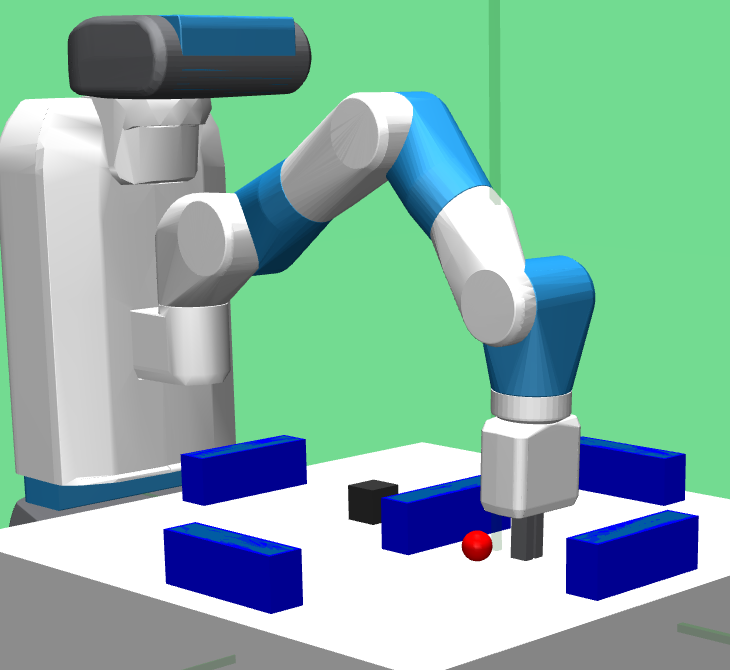
\includegraphics[width=0.4\linewidth]{figures/cmax/fetch.png}
%   %\end{subfigure}
%   \caption{4D Planar Pushing in the presence of obstacles. The task
%     is to push the black box to the red goal using the end-effector.}
%   \label{fig:simulation}
% \end{figure}

In this experiment, the task is for a robotic gripper to push a cube
from a start location to a goal location in the presence of
static obstacles without any resets, as shown in
Figure~\ref{fig:search} (right). This can be represented as a
planning problem in 4D continuous state space $\statespace$ with any state represented as
the tuple $s = (g_x,
g_y, o_x, o_y)$ where $(g_x, g_y)$ are the xy-coordinates of the
gripper and $(o_x, o_y)$ are the xy-coordinates of the object. The
model $\hat{M}$ used for planning \textit{does not} have the static obstacles and the
robot can only discover the state-action pairs that are affected due
to the obstacles through real world executions. The
action space $\actionspace$ is a discrete set of 4 actions that move
the gripper end-effector in the 4 cardinal directions by a fixed
offset using an IK-based controller. The cost of each transition is
$1$ when the object is not at the goal location, and $0$
otherwise.

\begin{table}[t]
  \centering
  \begin{tabular}{|c|c|c|c|c|}
    \hline
    & \multicolumn{2}{c|}{\textbf{Accurate Model}} &
                                                               \multicolumn{2}{c|}{\textbf{Inaccurate
                                                               Model}}
    \\
    \cline{2-5}
    & \textbf{Steps} & \textbf{\% Success} &
                                                    \textbf{Steps}
                          & \textbf{\% Success} \\
    \hline
    \textsc{Cmax} & $63 \pm 22$ & $90\%$ & $192 \pm 40$& $ 80\%$ \\
    \hline
    Q-Learning & $34 \pm 5$ & $90\%$ & $441 \pm 100$ & $45\%$\\
    \hline
    Model NN & $62 \pm 26 $&$90\%$&  $348 \pm 82$&$ 15\%$\\
    \hline
    Model KNN & $106 \pm 34 $&$95\%$& $533 \pm 118 $&$50\%$\\
    \hline
    \hline
    Plan with Accurate Model & $63 \pm 22 $&$90\%$ & $364 \pm 53 $&$85\%$\\
    \hline
  \end{tabular}
  \caption{Results for the simulated 4D planar pushing task. First
    column corresponds to the case when the environment has no
    obstacles, and the model is accurate. Second column corresponds to
    when the environment has static obstacles. and model (with no obstacles) is
    inaccurate. Each entry in the Steps subcolumn is obtained using $20$
    random start and goal locations, and we present mean and standard
    error of number of timesteps it takes the robot to reach the
    goal \textit{among successful trials}. The \% success subcolumn
    indicates percentage of successful trials where the robot reached the goal in less
    than 1000 timesteps. The last row corresponds to using the planner
  with an accurate model (the same as the environment.)}
\label{tab:fetch}

\end{table}

We compare \textsc{Cmax} with
the following baselines: a
model-free Q-learning approach
\cite{DBLP:journals/nature/MnihKSRVBGRFOPB15} that learns from
online executions in environment
and does not use the model $\hat{M}$, and a model learning approach that uses
limited-expansion search for planning but updates a learned residual that
compensates for the discrepancy in dynamics between the model and
environment. The model learning approach is very similar to previous works
that learn residual dynamics models and have been shown to work well in
episodic settings \cite{rastogi2018sample, DBLP:conf/icra/HaY15,
  DBLP:conf/iros/SaverianoYFL17}. We chose two function
approximators for the learned residual dynamics to account for
model learning approaches that use global function
approximators such as neural networks (NN)
\cite{DBLP:conf/nips/JannerFZL19}, and local function approximators
such as K-nearest neighbor regression (KNN)
\cite{DBLP:conf/nips/NouriL08, DBLP:conf/atal/JongS07}. Finally, we compare against
a limited-expansion search planner that uses an accurate model with
the full knowledge about
obstacles to understand the
difficulty of the task. Specific details on the architecture and baseline
parameters can be found in our original paper~\cite{cmax}.

For our implementation, we follow Algorithm~\ref{alg:large-state-spaces}
with euclidean distance metric, $\xi = 0.01$, and $\delta =
0.02$. These values are chosen to capture the discrepancies observed
in the object and gripper position when pushed into an obstacle, and the size of
the obstacles. We use the same values for the model learning KNN
baseline to ensure a fair comparison. The results of our experiments are
presented in Table~\ref{tab:fetch}. We notice that all the approaches
have almost the same performance when both model and environment have
no obstacles (first column). This validates that all the baselines
do well when the model is accurate. However, when the model is
inaccurate (second column), the performance varies across baselines.
Q-learning performs decently well since it relies on the model only
for the initialized Q-values and not during online executions, but as
the task is now more difficult, it solves much fewer trials and is
highly suboptimal. It is
interesting to see that model learning baselines do 
not do as well as one would expect. This can be attributed to the
number of online executions required to learn the correct residual,
which can be prohibitively large. Among 
the two model learning baselines, KNN works better since it requires
fewer samples to learn the residual, while NN requires large amounts of
data. In contrast, \textsc{Cmax} does not seek to learn the true
dynamics and instead is more focused on reaching the goal
quickly. When compared with a planner that uses the accurate model with
obstacles and solves $17$ trials (last row in Table~\ref{tab:fetch}),
our approach solves $16$ trials and achieves the lowest mean 
number of timesteps to reach the goal among all baselines.
We would like to note that the planner with accurate model takes a larger number of timesteps because
we used the same initial cost-to-go estimates as other approaches.
The initial cost-to-go estimates are more accurate for the model
with no obstacles than for the model with obstacles. Hence, it spends a
larger number of timesteps updating cost-to-go estimates.
% which are not near-optimal for the model with obstacles, but for the model
% with no obstacles.
This experiment shows that by focusing on reaching the goal and not
trying to correct the model 
dynamics, \textsc{Cmax} performs the best and solves the most number of
trials among baselines.

\begin{figure}[t]
  \centering
  % \begin{subfigure}{0.3\linewidth}
  %   \includegraphics[width=\linewidth]{figures/cmax/search.pdf}
  % \end{subfigure}
  % \hspace{10mm}
  % \begin{subfigure}{0.25\linewidth}
  %   \includegraphics[width=\linewidth]{figures/cmax/example.pdf}
  % \end{subfigure}
  {
  \begin{subfigure}{0.1\linewidth}
    \begin{tabular}{|c|c|c|}
      \hline
      & \textbf{Steps} & \textbf{\% Success} \\
      \hline
      \textbf{\textsc{Cmax}} & $47 \pm 6$&$ 100\%$ \\
      \hline
      \textbf{RTAA*} & $138 \pm 65 $&$ 30\%$ \\
      \hline
    \end{tabular}
  \end{subfigure}}
  \hspace{60mm}
  \begin{subfigure}{0.3\linewidth}
    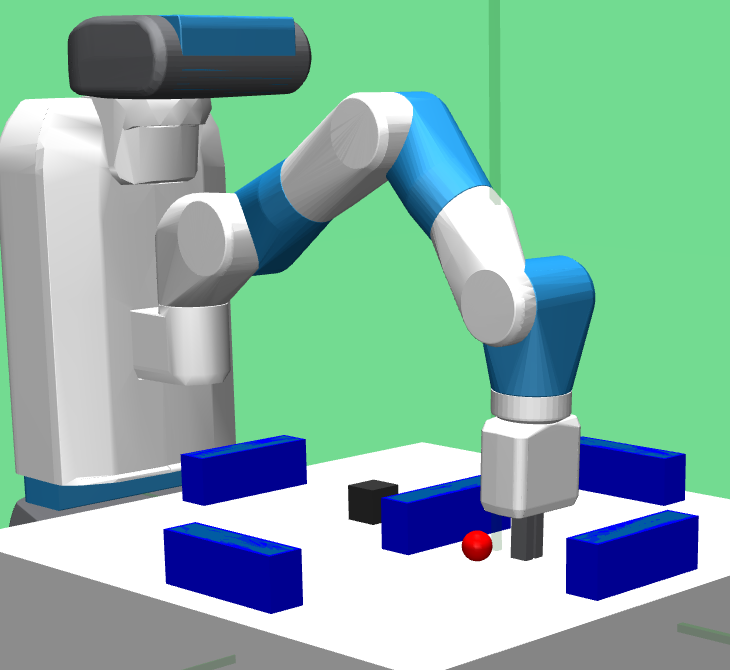
\includegraphics[width=\linewidth]{figures/cmax/fetch.png}
  \end{subfigure}
  \caption{(left) Results for simulated 7D arm planning experiment
    comparing RTAA* and \textsc{Cmax}. Each entry in the Steps column is obtained using 10
    trials with
    random start configurations and goal locations, and we present
    mean and standard error of number of timesteps it takes the arm to
    reach the goal \textit{among successful trials}. The \% success column
    indicates percentage of successful trials where the arm reached the
    goal in less than $300$ timesteps.(right)
    4D Planar Pushing in the presence of obstacles. The task
    is to push the black box to the red goal using the end-effector.}
  \label{fig:search}
  
\end{figure}

% \subsection{Simulated 7D Arm Planning with a Broken Joint}
% \label{sec:simulated-7d-arm}

% While the previous experiment tested our approach against popular
% baselines, this experiment is designed to evaluate the relative
% importance of the parameters involved in our algorithm. The task is to
% move a simulated 7D PR2 arm with a broken joint from a start
% configuration so that the end-effector reaches a desired 3D goal
% region without any resets, as shown in Figure~\ref{fig:simulation}(right). This can be represented as a
% planning problem in 7D discrete state space $\statespace$ where each
% dimension corresponds to a joint of the arm bounded by the joint
% limits. In this experiment, we discretize each dimension into $10$ bins and plan in the
% resulting discrete state space of size $10^7$. The action space
% $\actionspace$ is a discrete set of size $14$ corresponding to moving
% each joint by a fixed offset in the positive or negative direction. We
% use an IK-based controller to navigate between states. The model
% $\hat{M}$ used for planning \textit{does not} know that a joint is
% broken and assumes that the arm can be moved to any configuration
% within the joint limits. In the real world, if the robot tries to move
% the broken joint, the arm does not move. Thus, the robot realizes the
% unattainable configurations only through real world executions. The
% cost of each transition is the distance of end-effector from the goal
% region. Since planning in 7D can be computationally expensive and
% potentially take a long time, we use a weighted version of
% limited-expansion search proposed in
% \cite{DBLP:journals/ai/RiveraBH15} which simply modifies the
% cost-to-go update as $V(s') \leftarrow w(g(s_{\mathsf{best}}) - g(s'))
% + V(s_{\mathsf{best}})$, where $w \geq 1$ is a constant weight. It has been
% empirically shown that using the weighted update results in speedup in
% time taken to reach the goal. We use the weighted update with a weight
% of $w = 32$ in this experiment.

% We vary two parameters of Algorithm~\ref{alg:large-state-spaces} with
% the manhattan distance metric:
% discrepancy threshold $\xi$, and radius of the hyperspheres
% $\delta$. The aim of this experiment is to understand the effect of
% these parameters on the performance of our approach. In addition to
% this, we also measure the effectiveness of function approximation used
% for cost-to-go updates in comparison to exact updates like the ones
% performed by Algorithm~\ref{alg:small-state-spaces}, RTAA*, and other
% real-time search methods. For this experiment, we use a RBF kernel
% regressor with L2 regularization for the function approximation of
% cost-to-go estimates, and all trials start with the same initial
% cost-to-go estimates. The results of our experiments are presented in
% \anirudh{present and discuss results}.

\subsection{3D Pick-and-Place with a Heavy Object}
\label{sec:real-world-3d}

\begin{figure*}[t]
  \centering
  \begin{subfigure}{0.13\linewidth}
    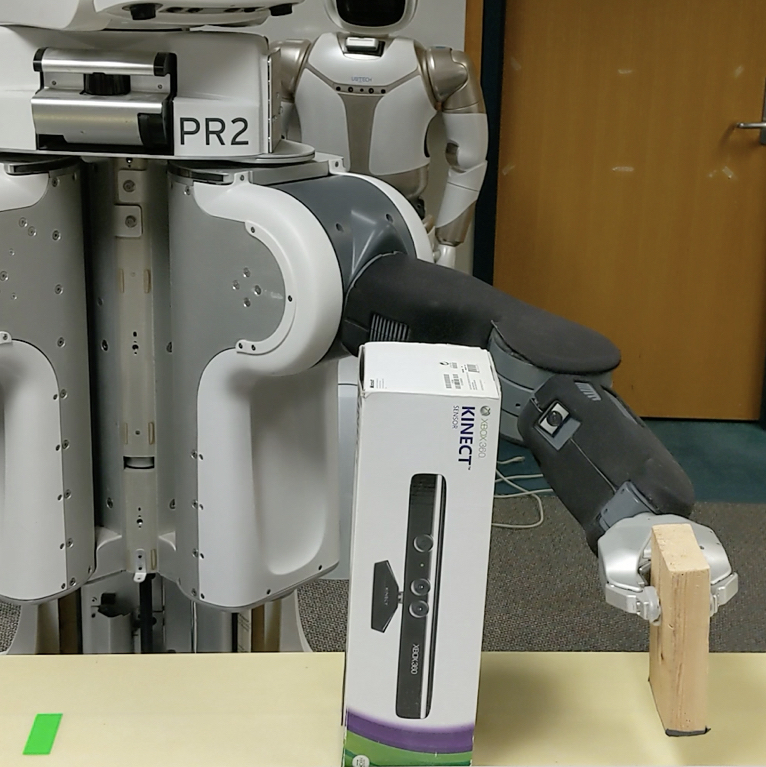
\includegraphics[width=\linewidth]{figures/cmax/pr2_pick_place_light_1_annotated.jpeg}
  \end{subfigure}
  \begin{subfigure}{0.13\linewidth}
    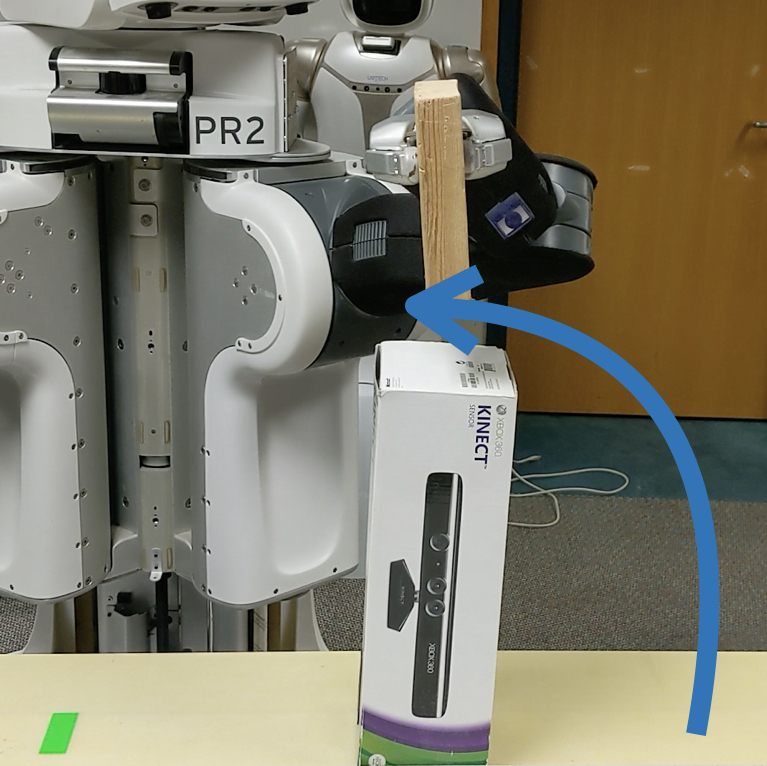
\includegraphics[width=\linewidth]{figures/cmax/pr2_pick_place_light_2_annotated.jpeg}
  \end{subfigure}
  \begin{subfigure}{0.13\linewidth}
    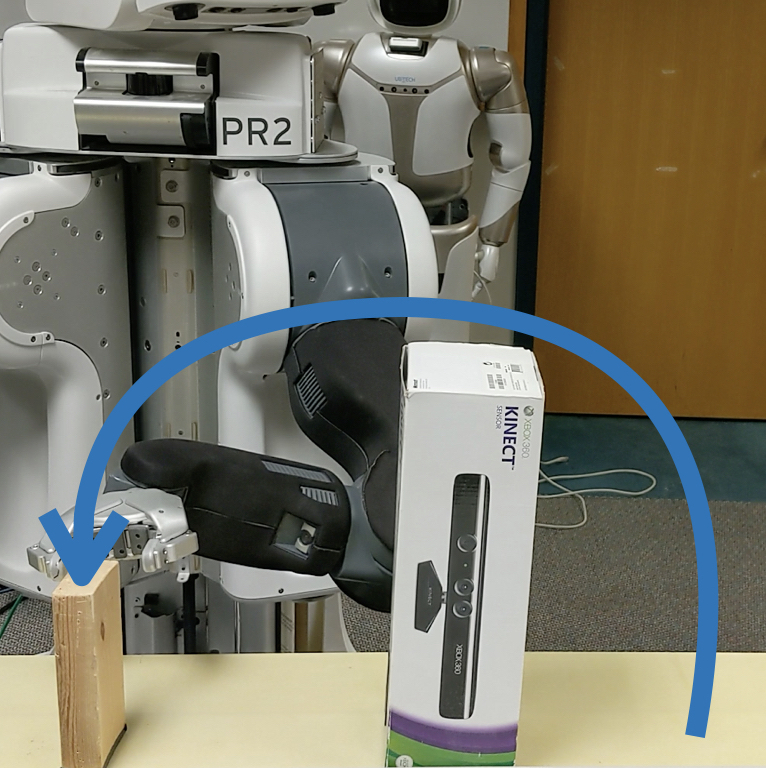
\includegraphics[width=\linewidth]{figures/cmax/pr2_pick_place_light_3_annotated.jpeg}
  \end{subfigure}
  \begin{subfigure}{0.13\linewidth}
    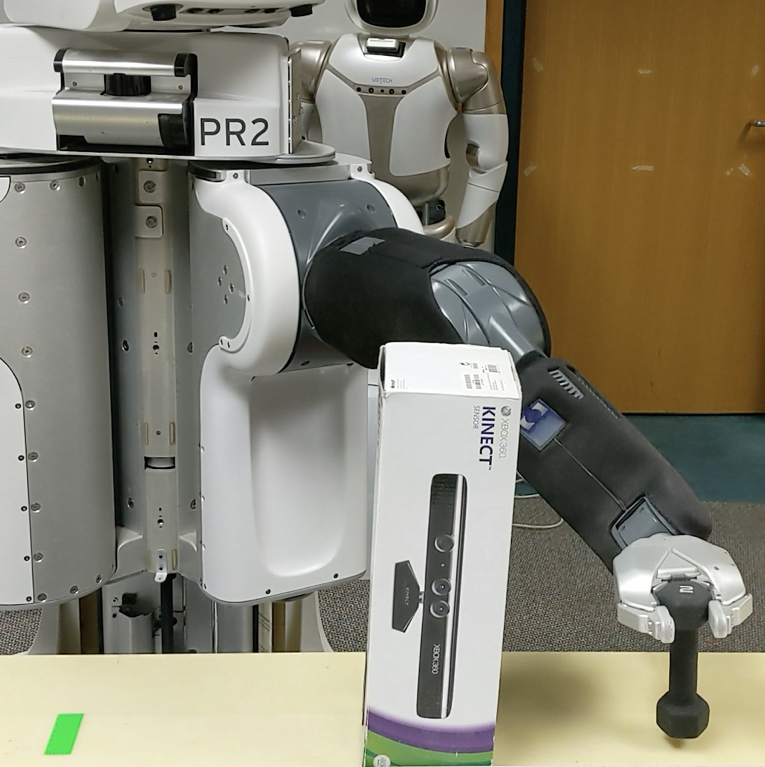
\includegraphics[width=\linewidth]{figures/cmax/pr2_pick_place_heavy_1_annotated.jpeg}
  \end{subfigure}
  \begin{subfigure}{0.13\linewidth}
    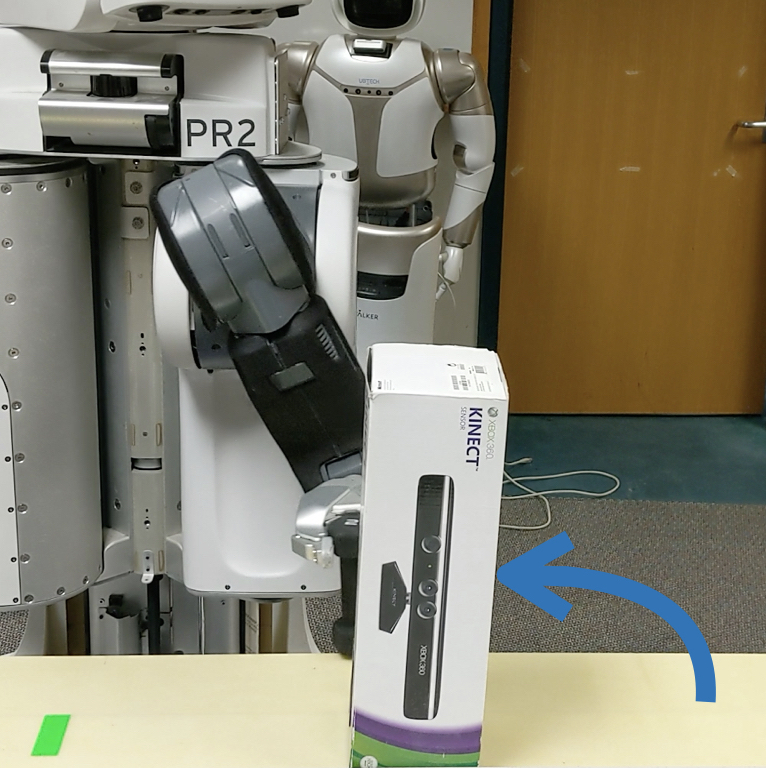
\includegraphics[width=\linewidth]{figures/cmax/pr2_pick_place_heavy_2_annotated.jpeg}
  \end{subfigure}
  \begin{subfigure}{0.13\linewidth}
    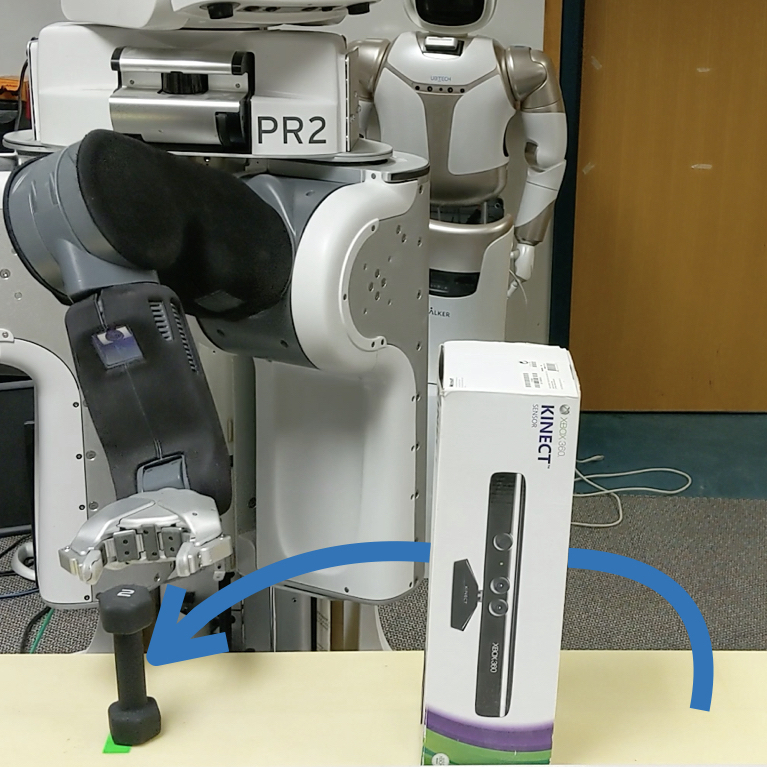
\includegraphics[width=\linewidth]{figures/cmax/pr2_pick_place_heavy_3_annotated.jpeg}
  \end{subfigure}
  \begin{subfigure}{0.13\linewidth}
    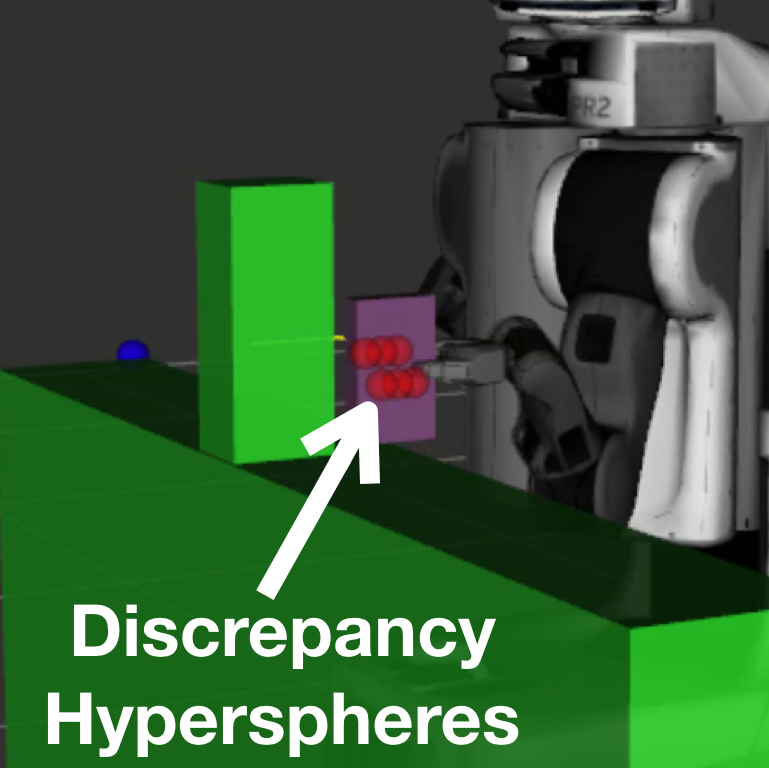
\includegraphics[width=\linewidth]{figures/cmax/pr2_pick_place_rviz_cropped_annotated.jpeg}
  \end{subfigure}
  \caption{Physical robot 3D pick-and-place experiment. The task is to
    pick the object (light - wooden block, heavy - black dumbbell) and
    place it at the goal location (green) while avoiding the obstacle
    (box). For the light object (first 3 images), the model dynamics are accurate and
    the robot takes it on the optimal path that goes above the
    obstacle. For the heavy object (next 3 images), the model dynamics are
    inaccurate but using \textsc{Cmax} the robot discovers that there
    is a discrepancy in dynamics when the object is lifted beyond a
    certain height (due to joint torque limits), adds hyperspheres at
    that height to
    account for these transitions (red spheres in the last image), and quickly finds an
    alternate path going behind the obstacle.}
  \label{fig:real-3d}
  
\end{figure*}

The task of this physical robot experiment (Figure~\ref{fig:real-3d}) is to pick and place a heavy 
object using a PR2 arm from a start pick location to a goal place
location while avoiding an obstacle. This can be represented as a
planning problem in 3D discrete state space $\statespace$ where
each state corresponds to the 3D location of the end-effector.
% In our
% experiment, we discretize each dimension into $20$ bins and plan in
% the resulting discrete state space of size $20^3$.
Since it is a
relatively small state space, we use exact planning updates without
any function approximation following
Algorithm~\ref{alg:small-state-spaces} with $K=3$ expansions.
The action space is a
discrete set of $6$ actions corresponding to a fixed offset movement
in positive or negative direction along each dimension.
% We use a
% RRT-based motion planner \cite{DBLP:journals/ijrr/LaValleK01} to plan the path of the
% arm between states, while avoiding collision with the obstacle.
The
model $\hat{M}$ used by planning \textit{does not} model the object as
heavy and hence, does not capture the dynamics of the arm correctly when it
holds the heavy object. Specific details regarding the experiment can
be found in our original paper~\cite{cmax}.
% The cost of each transition is $1$ if 
% object is not at the goal place location, otherwise it is $0$.

We observe that if the object was not heavy, then the arm takes the
object from the start pick location to the goal place location on the
optimal path which goes above the obstacle (first 3 images of
Figure~\ref{fig:real-3d}). However, when executed
with a heavy object, the arm cannot lift the object beyond a certain
height as its joint torque limits are reached. At this point, the robot notes the
discrepancy in dynamics between the model $\hat{M}$ and the real world,
and inflates the cost of any executed transition that tried to move the object
higher. Subsequently, the robot figures out
an alternate path that does not require it to lift the object higher
by taking the object behind the obstacle to the goal place
location (last 4 images of Figure~\ref{fig:real-3d}). The robot takes
36 timesteps (25.8 seconds) to reach
the goal with the heavy object, in comparison to 26 timesteps (22.8 seconds) for the
light object (see video). Thus, the robot using \textsc{Cmax} successfully completes the task despite having a
model with inaccurate dynamics.

\subsection{7D Arm Planning with a Non-Operational Joint}
\label{sec:real-world-7d}

\begin{figure}[t]
  \centering
  \begin{subfigure}{0.3\linewidth}
    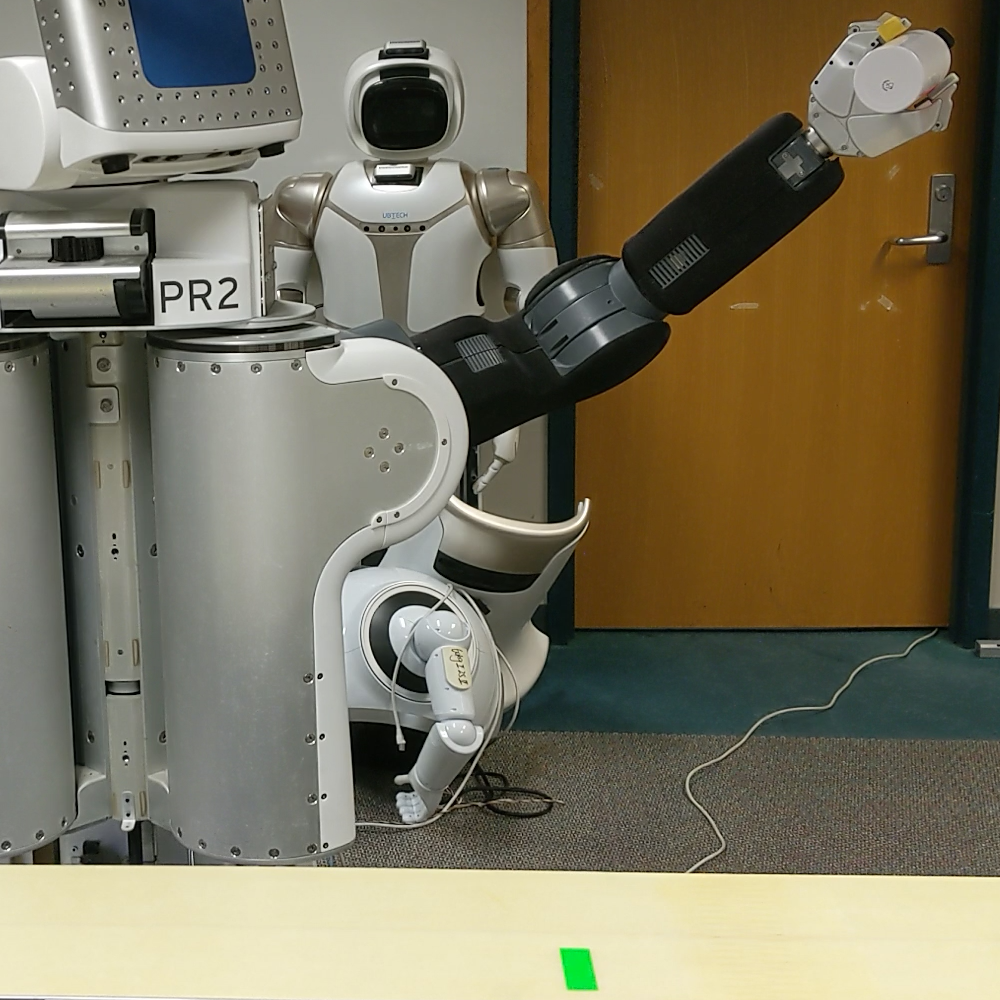
\includegraphics[width=\linewidth]{figures/cmax/pr2_place_initial.png}
  \end{subfigure}
  \begin{subfigure}{0.3\linewidth}
    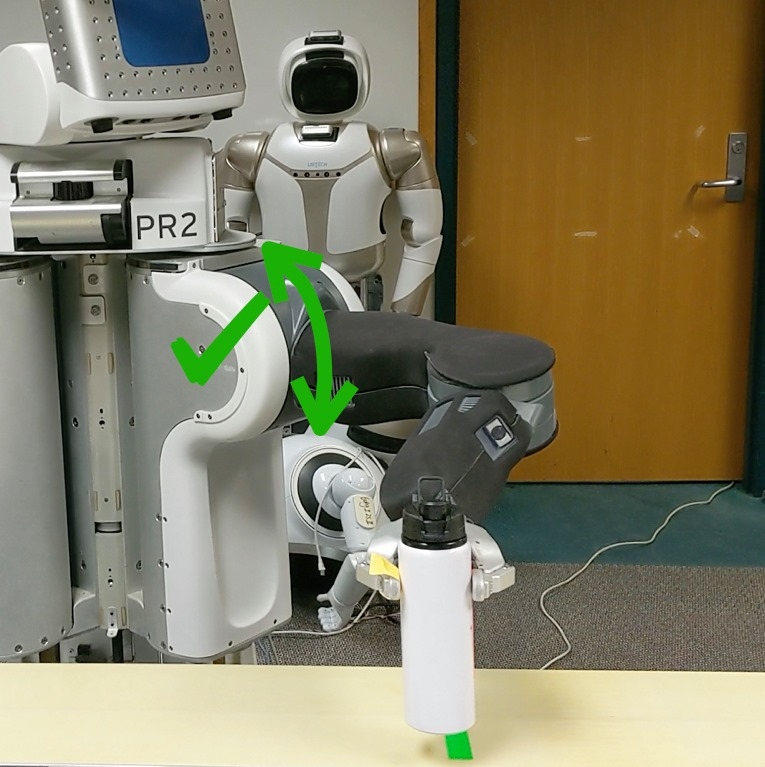
\includegraphics[width=\linewidth]{figures/cmax/pr2_place_working_final_annotated_thicker.jpg}
  \end{subfigure}
  \begin{subfigure}{0.3\linewidth}
    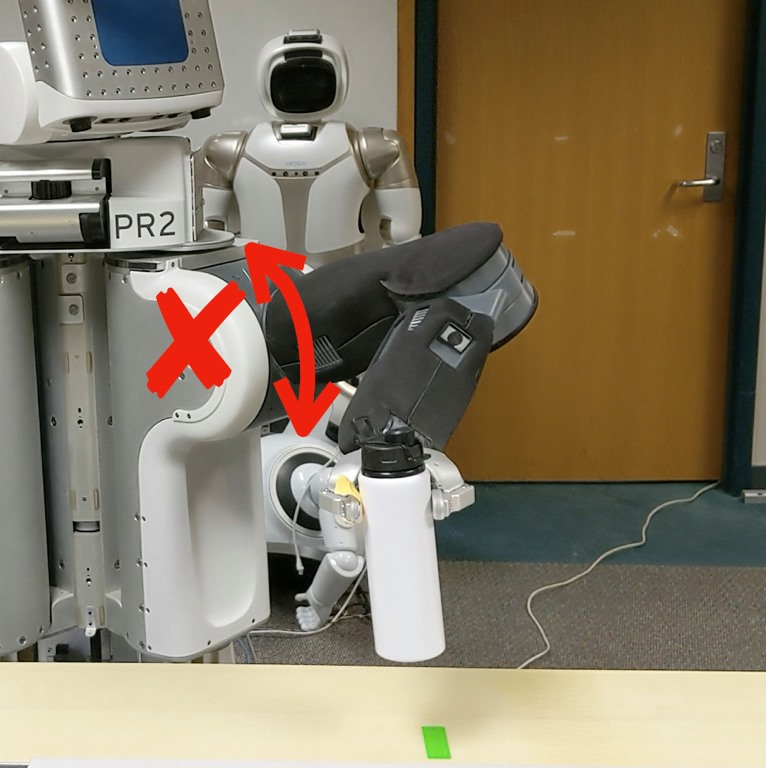
\includegraphics[width=\linewidth]{figures/cmax/pr2_place_broken_final_annotated_thicker.jpg}
  \end{subfigure}
  \caption{Physical robot 7D arm planning experiment. The task is to start
  from a fixed configuration (shown in the first image) and move the
  arm so that the end-effector reaches the object place location
  (green). When the shoulder lift joint is operational, the robot uses
  the joint to quickly find a path to the goal (middle image). However, when the
  joint is non-operational, it encounters discrepancies in its model
  and compensates by finding a path that uses other joints to reach
  the goal (last image.)}
  %In the first 3 images, all joints are
% working and the robot finds a path that uses the shoulder lift joint
% to decrease the height of the end-effector and reach the goal
% region. However, in the last 3 images, the shoulder lift joint is
% broken and the robot discovers that any action that tries to move that
% joint results in a discrepancy in dynamics resulting in a path that
% uses other joints such as shoulder pan joint and elbow flex joint to
% decrease the height of the end-effector and still reach the goal
% region successfully.}
\label{fig:real-7d}

\end{figure}

The task of this physical robot experiment (Figure~\ref{fig:real-7d}) is
to move the PR2 arm with a
non-operational joint from a start configuration so that the
end-effector reaches a goal location, specified as a 3D
region. We represent this as a planning problem in 7D
discrete statespace $\statespace$ where each dimension corresponds to
a joint of the arm bounded by its joint limits. The action space
$\actionspace$ is a discrete set of size 
$14$ corresponding to moving each joint by a fixed offset in the
positive or negative direction. The model $\hat{M}$ used for
planning \textit{does not} know that a joint is non-operational and
assumes that the arm can attain any configuration within the joint
limits. In the real world, if the robot tries to move the
non-operational joint, the arm does not move. Specific details regarding the experiment can
be found in our original paper~\cite{cmax}.
% We use a
% weighted version of
% limited-expansion search proposed in
% \cite{DBLP:journals/ai/RiveraBH15} which modifies the
% cost-to-go update as $V(s') \leftarrow w(g(s_{\mathsf{best}}) - g(s'))
% + V(s_{\mathsf{best}})$, where $w \geq 1$ is a constant weight. It has been
% empirically shown that using the weighted update results in a speedup in
% time taken to reach the goal.

For the purpose of this
experiment since the state space is very large, we follow Algorithm~\ref{alg:large-state-spaces} with $\delta
= 1$, $\xi = 1$, and make the shoulder lift joint (marked by red cross and arrows
in last image of Figure~\ref{fig:real-7d}) of PR2 non-operational. We use a
kernel regressor with RBF kernel of length scale $\gamma = 10$ for
the cost-to-go function approximation. Figure~\ref{fig:real-7d} shows \textsc{Cmax} operating in the
real world to place an object at a desired location with a goal
tolerance of $10$ cm. When the shoulder lift joint is operational, the robot finds a
path quickly to the place location by using the joint (middle image of
Figure~\ref{fig:real-7d}). However, when the shoulder lift joint is
non-operational, the robot notes discrepancy in dynamics whenever it tries to
move the joint, places hyperspheres in 7D to inflate the cost, and
comes up with an alternate path (last image of
Figure~\ref{fig:real-7d}) to reach the place location. The 
robot takes $13$ timesteps (32.4 seconds) to reach the goal location with the
non-operational joint, in comparison to $10$ timesteps (25.8 seconds) for the case
where the joint is working (see video). Thus,
the robot successfully finds a path to the place location despite using a
model with inaccurate dynamics.

To emphasize the need for cost-to-go function approximation and
local generalization from hyperspheres in large state spaces, we compared \textsc{Cmax}
against RTAA*, an exact planning method that uses a tabular
representation for cost-to-go estimates and updates model dynamics
online. Results are presented in 
Figure~\ref{fig:search} (left) and show that RTAA* fails to solve $7$
of the $10$ trials whereas \textsc{Cmax} solves all of them, and in
smaller mean number of timesteps.

%\subsection{Simulated 7D Arm Planning with a Non-Operational Joint}
%\label{sec:simulated-7d-arm-2}

\subsection{Effect of Function Approximation and Size of Hyperspheres}
\label{sec:underst-effect-funct}
\begin{figure}[t]
  \centering
  \begin{subfigure}{0.4\linewidth}
    \includegraphics[width=\linewidth]{figures/cmax/gamma.pdf}
  \end{subfigure}
  \hspace{10mm}
  \begin{subfigure}{0.4\linewidth}
    \includegraphics[width=\linewidth]{figures/cmax/radius.pdf}
  \end{subfigure}
  \caption{(left) Performance of \textsc{Cmax} for 7D arm planning as
    the smoothness of the cost-to-go function approximator varies. The plot is
    generated for each value of length scale $\gamma$ by generating
    $10$ random start configurations and goal locations, and running
    our approach for a maximum of $100$ timesteps. (right) Performance
    of our approach for 4D planar pushing as the radius of the
    hypersphere $\delta$ varies. The plot is generated for each value
    of radius $\delta$ by generating $10$ random start and goal
    locations, and running \textsc{Cmax} for a maximum of $400$ timesteps.}
  \label{fig:gamma-radius}
  
\end{figure}

While previous experiments have tested \textsc{Cmax} against other
baselines and on a physical robot, this experiment is designed to
evaluate the effect of cost-to-go function approximation and the size
of hyperspheres on the
performance of \textsc{Cmax} in large state spaces (Algorithm~\ref{alg:large-state-spaces}.)
For the first set of experiments (Figure~\ref{fig:gamma-radius} left), we use the setup of
Section~\ref{sec:real-world-7d} and focus on varying the smoothness of the kernel
regressor cost-to-go function approximation
by varying the length scale $\gamma$ of the RBF kernel.
Intuitively, small length scales result in approximation with high
variance, and for large scales we obtain highly smooth approximation.
% For small length
% scales, the resulting approximation has very high variance and 
% resembles the behavior of maintaining a tabular representation for
% cost-to-go estimates (like Algorithm~\ref{alg:small-state-spaces}), and for large length scales the resulting
% approximation is highly smooth and could potentially fail at distinguishing
% the relative importance of nearby states.
% We record the number of timesteps over 10 random start
% configurations and goal locations as we vary the length scale
% $\gamma$.
We notice that for small $\gamma$, the performance is poor and
as $\gamma$ increases, the performance of \textsc{Cmax}
becomes better as it can generalize the cost-to-go estimates
in the state space. However, for large $\gamma$ the performance
deteriorates as it fails to capture the difference in cost-to-go
values among nearby states due to excessive smoothing. This showcases
the need for generalization in cost-to-go
estimates for efficient updates in large state spaces.

For the second set of experiments (Figure~\ref{fig:gamma-radius}
right), we vary the radius of the 
hyperspheres $\delta$ introduced whenever an incorrect
state-action pair is discovered in
Algorithm~\ref{alg:large-state-spaces}. We use the setup of
Section~\ref{sec:simulated-4d-planar}, vary 
$\delta$ and observe the number of timesteps it takes the robot to
push the object to the goal. We observe that when $\delta$ is
large, the performance is poor as we potentially penalize state-action
pairs that are not incorrect and could result in a very suboptimal
path. However, a very small $\delta$ can also lead to a poor
performance, as we need more online executions to discover the set of
incorrect state-action pairs. Hence, the radius $\delta$ needs to be
chosen carefully to quickly ``cover'' the incorrect set, while not
penalizing any correct state-action pairs.

\subsection{Simulated 2D Gridworld Navigation with Icy States}
\label{sec:simul-2d-gridw}

% \begin{table}[t]
%   \centering
%   \begin{tabular}{|c|c|c|c|}
%     \hline
%     \textbf{\% obstacles}& \textbf{0\%} & \textbf{40\%}
%     &\textbf{80\%} \\
%     \hline
%     \textbf{Our Approach} & $78 \pm 4 $  & $1551
%                                                                 \pm
%                                                                 373
%                                                                 $
%     & $138 \pm 10 $ \\
%     \hline
%     \textbf{Adaptive} & $78 \pm 4 $  &
%                                                                   $1015
%                                                                   \pm
%                                                                   230
%                                                                   $
%      & $137 \pm 10 $ \\
%     \hline
%     \textbf{Q-Learning} & $3879 \pm 305 $ 
%                                                              &
%                                                                $11803
%                                                                \pm
%                                                                2542
%                                                                $
%      & $510 \pm 36 $ \\
%     \hline
%     % \textbf{Eps-Greedy} & $90 \pm 5 $  & $4311
%     %                                                           \pm
%     %                                                           1941
%     %                                                           (18)$
%     % & $12405 \pm 2362 (45)$\\
%     % \hline
%   \end{tabular}
%   \caption{Results for gridworld navigation in presence of
%     obstacles for a grid of size $100 \times 100$. Each entry is obtained using 50 random seeds and we
%     present the mean and standard error of the number of timesteps it
%     takes the robot to reach the goal.
%     % Numbers in parenthesis indicate
%   % the number of trials among the 50 trials where the robot reached the goal in less than
%   % $100000$ timesteps.
% }
%   \label{tab:obstacle}
% \end{table}

\begin{table}[t]
  \centering
  \begin{tabular}{|c|c|c|c|}
    \hline
    \textbf{\% Ice} $\rightarrow$& \textbf{0\%} & \textbf{40\%}
    & \textbf{80\%} \\
    \hline
    \textsc{Cmax} & $78 \pm 4 $ & $231
                                                                \pm
                                                                18
                                                                $
    & $2869 \pm 331 $ \\
    \hline
    RTAA* & $78 \pm 4 $  &
                                                                  $219
                                                                  \pm
                                                                  18
                                                                  $
    & $2185 \pm 249 $ \\
    \hline
    Q-Learning & $3914 \pm 303 $ &
                                                               $1220
                                                               \pm
                                                               103
                                                               $
    & $996 \pm 108 $ \\
    \hline
    % \textbf{Eps-Greedy} & $89 \pm 53 $ & $7814
    %                                                           \pm
    %                                                           2600
    %                                                           (42/50)$
    % & $3177 \pm 1700 (5/50)$\\
    % \hline
  \end{tabular}
  \caption{Results for gridworld navigation in presence of
    icy states for a grid of size $100 \times 100$. Each entry is obtained using 50 random seeds, and we
    present the mean and standard error of the number of timesteps it
    takes the robot to reach the goal. The columns represent the
    percentage of icy states in the gridworld.
    % Numbers in parenthesis indicate
  % the number of trials where the robot reached the goal in less than
  % $100000$ timesteps.
}
\label{tab:icy}
\end{table}

In our final experiment, we want to understand the performance of \textsc{Cmax}
compared to other baselines in small domains where model dynamics
can be represented using a table, and can be updated efficiently.
We consider the 2D gridworld such
as the one shown in Figure~\ref{fig:intro}(right) with icy
states where the robot slips (moving left or right on ice moves the
robot by two cells.) The model used for planning
\textit{does not} contain ice, and is an
empty gridworld.
% Random gridworlds with ice
% of size $100 \times 100$ are generated, with random start and goal
% locations for the robot, and we compare \textsc{Cmax}
% (Algorithm~\ref{alg:small-state-spaces}) with the following baselines:
% Adaptive RTAA*, and Q-learning, a model-free baseline that learns solely
% from online executions.
% and Eps-greedy, an approach that executes
% random actions with small probability and executes the best action
% predicted by limited-expansion planner otherwise.
The results are
presented in Table~\ref{tab:icy}. We can observe that model-free approaches like
Q-learning perform well compared to model-based approaches in cases where the model available is
highly inaccurate (see Table~\ref{tab:icy} last column.) However, when
the model is reasonably accurate
RTAA* performs the best. But the
results show that even in domains where model 
dynamics are simple and can be updated efficiently, \textsc{Cmax} competes closely
with RTAA*. Thus, our approach is still applicable in such
domains and is relatively easier to implement.

\section{Related Work}
\label{sec:related-work}

The proposed approach has components concerning real-time heuristic
search, local function approximation methods, and dealing with
inaccuracy in models. There is a wide array of existing work at the
intersection of planning and learning that deal with these
topics. Notably, we leverage prior 
work on real-time heuristic search \cite{DBLP:journals/ai/Korf90,
  DBLP:conf/atal/KoenigL06} for the limited-expansion search-based
planner presented in
Algorithm~\ref{alg:limited-expansion-search}. Using local function
approximation methods in
robotics has been heavily explored in seminal works \cite{
DBLP:conf/icml/VijayakumarS00, DBLP:conf/icra/AtkesonS97} due to their smaller sample complexity
requirements and local generalization properties that do not cause
interference \cite{DBLP:journals/air/AtkesonMS97a,
  DBLP:conf/icml/CoatesAN08}. More recently,
\cite{DBLP:conf/atal/JongS07}, 
\cite{DBLP:conf/nips/NouriL08} and \cite{DBLP:journals/ml/BernsteinS10} have also proposed approaches that
learn local models from online executions. However unlike \textsc{Cmax},
they use these models to approximate the dynamics of the real world. Our work is also closely related to
the field of real-time reinforcement learning that tackles the problem
of acting near-optimally in unknown environments, without any resets~\cite{DBLP:journals/sigart/Sutton91, DBLP:journals/ai/BartoBS95, DBLP:conf/aaai/KoenigS93}. The analysis presented in
Theorem~\ref{thm:small-state-spaces} and \ref{thm:large-state-spaces} borrows several useful results
from \cite{DBLP:conf/aaai/KoenigS93}. Prior
works in model-based reinforcement learning with provable guarantees,
such as \cite{DBLP:journals/ml/KearnsS02, DBLP:journals/ml/BernsteinS10,
  DBLP:journals/jmlr/BrafmanT02, DBLP:conf/icml/KakadeKL03}, are also
related. However, these works learn the true
dynamics by updating the model and give sample complexity results in
the finite-horizon setting or discounted infinite-horizon setting,
unlike our shortest path setting. Among these works,
\cite{DBLP:conf/icml/KakadeKL03}, which proposes a method for exploration in metric
state spaces, serves as an inspiration for the covering number
bounds given in
Theorem~\ref{thm:large-state-spaces}. The work that is most closely
related to ours is \cite{DBLP:conf/aaai/Jiang18}
which proposed an approach that uses a similar idea of updating the cost
function, in cases where updating the model dynamics is infeasible. However, their
approach is suitable only for episodic settings and small state
spaces. Concurrent work by \cite{DBLP:journals/ral/McConachiePMB20}
employs a binary classifier trained on offline data to predict whether
a transition is incorrect or correct, that is then queried during
online motion planning to construct the search tree consisting of only
transitions that are classified as correct.
% We
% extend it to the challenging online real-time setting and provide an
% algorithm for large state spaces. 

\section{Discussion and Conclusion}
\label{sec:discussion}
\textsc{Cmax} is the first approach for interleaving planning and
execution that does not require updating 
dynamics, and is guaranteed to reach the goal despite
using an inaccurate dynamical model.
The biggest advantage of \textsc{Cmax} is
that it does not rely on any knowledge of how the model is inaccurate, and
whether it can be updated in real-time.
% whether the model dynamics can be updated in
% real-time, or knowledge of how the model is inaccurate and ways to
% correct it.
Hence, it
is broadly applicable in real world robotic tasks with complex inaccurate
models.
In domains where modeling the true dynamics is
intractable, such as deformable manipulation, \textsc{Cmax} can still
be employed to ensure successful execution.
% In our experiments, we have tested on several
% high-dimensional robotic tasks ranging from 4D planar pushing to
% 3D pick-and-place to 7D arm planning, which shows the versatility of
% \textsc{Cmax}.
In comparison, approaches that update the model dynamics
online rely on the flexibility of the model to be updated, knowledge
of what is lacking in the model, and a large number of online
executions to correct it. For example, to learn accurate dynamics for a transition
in $N$-D statespace we need at least $N$ samples in the worst case,
whereas our approach needs only $1$ sample to observe a discrepancy
and inflate the cost. The most important shortcomings of \textsc{Cmax}
are
Assumptions~\ref{assumption:core} and \ref{assumption:core-large},
which are hard to verify, and are not satisfied in several real world
robotic
tasks. For
example, consider the task of opening a spring-loaded door 
which is not modeled as loaded. All transitions would have discrepancy in
dynamics, and \textsc{Cmax} as is would fail at completing the task
in a reasonable amount of time. In addition, the hyperparameter
$\delta$ describing the radius of hypersphere needs to be
tuned carefully for each domain which is a limitation of \textsc{Cmax}.

To summarize, we present \textsc{Cmax} for interleaving planning
and execution using inaccurate models that does not require updating
the dynamics of the model, and still provably completes the task. We
propose practical algorithms for both small and large state spaces,
and deploy them successfully in real world robot tasks showing its broad
applicability. In simulation, we 
analyze \textsc{Cmax} and show that it outperforms baselines that
update dynamics online.
% Future directions include establishing
% similar guarantees like Theorem~\ref{thm:large-state-spaces} in the
% approximate planning setting, and relaxing
% Assumptions~\ref{assumption:core}, \ref{assumption:core-large} so that
% \textsc{Cmax} is applicable to a wider range of robotic tasks.

%%% Local Variables:
%%% mode: latex
%%% TeX-master: "../main"
%%% End:

\chapter{Leveraging Experience in Planning and Execution
  using Inaccurate Models}
\label{cha:lever-exper}

\epigraph{\textit{\ldots many of mundane manipulation tasks
such as picking and placing various objects in a kitchen are
highly repetitive. It is therefore expected that robots should
be capable of learning and improving their performance with
every execution of these repetitive tasks.}}{Mike Phillips, Ben Cohen,
Sachin Chitta, Max Likhachev (2012)}

While \cmax{}, presented in Chapter~\ref{cha:plann-exec}, guaranteed
task completeness using inaccurate models, it required strong
assumptions on the accuracy of the model. Furthermore, in a repetitive
task where the robot is required to complete the same task over
several repetitions, \cmax{} fails to improve the solution quality and
in some cases, fails to complete the task in later repetitions. This
chapter presents an algorithm that avoids this behavior by leveraging
the online experience to improve quality of solution across
repetitions while retaining task completeness guarantee in each
repetition. These guarantees require a milder assumption on the
accuracy of the model which is easier to satisfy when compared to the
assumption required by \cmax{}. However, like \cmax{}, the proposed
algorithm does not require any updates to the dynamics of the model
and only adapts the behavior of the planner in the spirit of this thesis.

\section{Introduction}
\label{sec:introduction}

We often require robots to perform tasks that are highly repetitive,
such as picking and placing objects in assembly tasks and navigating
between locations in a warehouse. For such tasks,
robotic planning algorithms have been highly effective in cases where
system dynamics is easily specified by an efficient forward
model~\cite{DBLP:conf/icra/BerensonAG12}. However, for
tasks involving interactions with objects, dynamics are very
difficult to model without
complete knowledge of the parameters of the
objects such as mass and friction~\cite{DBLP:journals/ijrr/JiX01}. 
Using
inaccurate models for planning can result in plans
that are ineffective and fail to complete the
task~\cite{DBLP:journals/ral/McConachiePMB20}. 
In addition for such
repetitive tasks, we expect the robot's task performance to
improve, leading to efficient plans in later repetitions.
Thus, we need
a planning approach that can use potentially inaccurate models while leveraging
experience from
past executions to complete the task in each repetition, and improve
performance across repetitions.


\begin{figure}[t]
  \centering
  \begin{subfigure}{.4\columnwidth}
    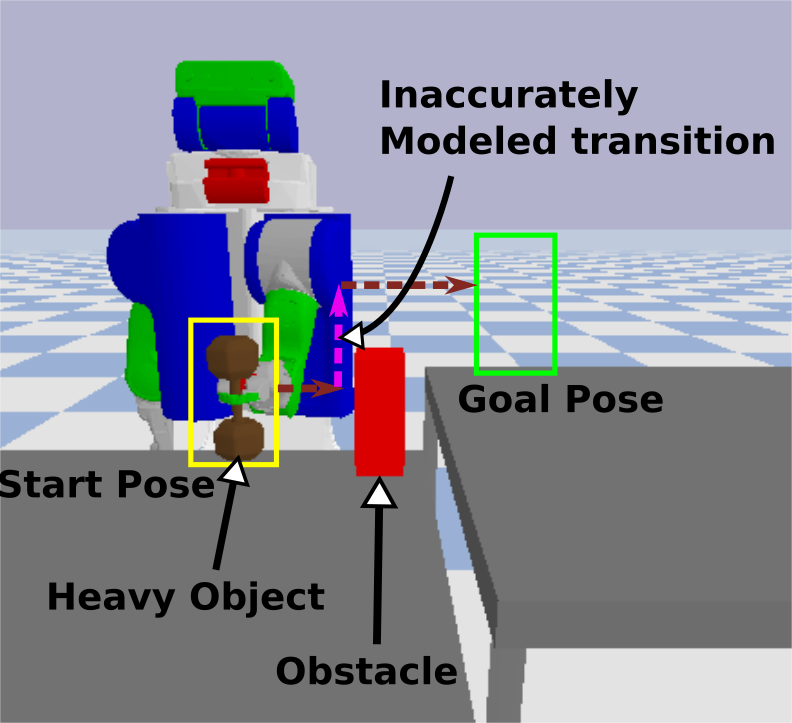
\includegraphics[width=\linewidth]{figures/cmaxpp/intro_grasp_new.png}
  \end{subfigure}
  \hspace{10mm}
  \begin{subfigure}{.4\columnwidth}
    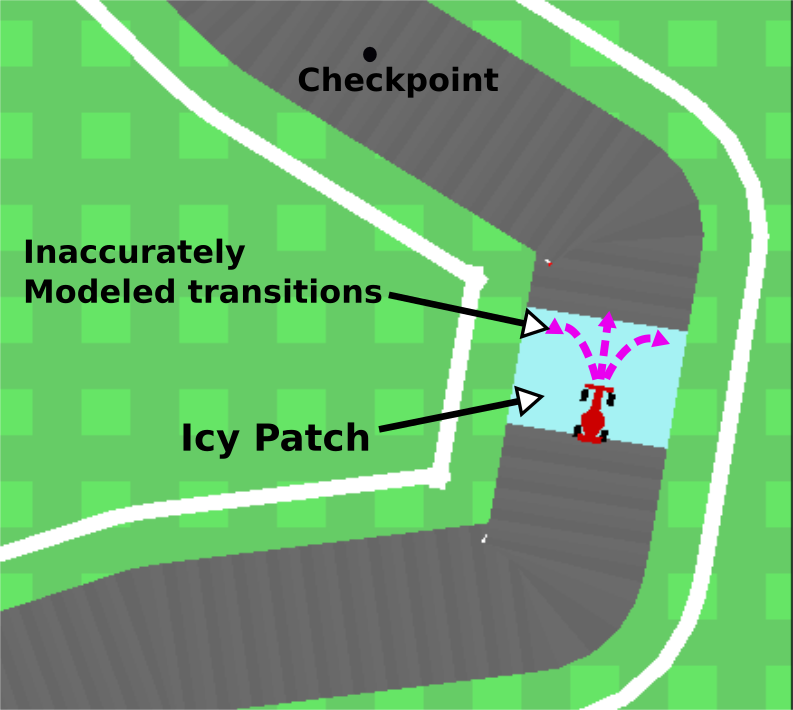
\includegraphics[width=\linewidth]{figures/cmaxpp/intro_car_new.png}
  \end{subfigure} 
  \caption{(left) PR2 lifting a heavy dumbbell, that is modeled as
    light, to a goal location that is higher than the start location
    resulting in dynamics that are inaccurately modeled (right) Mobile robot
    navigating around a track with icy patches with unknown friction parameters
    leading to the robot skidding. In both cases, any path to the goal
    needs to contain a
    transition (pink) whose dynamics are not modeled accurately.}
  \label{fig:intro}
\end{figure}

A recent planning approach, \cmax{}, introduced
in~\cite{cmax} adapts its planning strategy online to account
for any inaccuracies in the forward model without requiring any
updates to the dynamics of the model. \cmax{} achieves this online by
inflating the cost of any transition that is found to be incorrectly
modeled and replanning, thus biasing the resulting plans away from
regions where the model is inaccurate. It does so while maintaining
guarantees on completing the task, without any resets, in a finite
number of executions. However, \cmax{} requires
that there always exists a path from the current state of the robot to the goal
containing only transitions that have not yet been found to be incorrectly
modeled. This is a strong assumption on the accuracy of the model and
% is often not satisfied in several repetitive robotic tasks.
can often be violated, especially in the context of repetitive tasks.

For example, consider the task shown in Figure~\ref{fig:intro}(left)
where a robotic arm needs to repeatedly pick a heavy object, that is
incorrectly modeled as light, and place it on top of a taller table while avoiding
an obstacle. As the object is heavy, transitions that involve lifting
the object will have discrepancy between true and modeled
dynamics. However, any path from the start pose to the goal pose
requires lifting the object and thus, the resulting plan needs to
contain a transition that is incorrectly modeled. This violates the
aforementioned assumption of \cmax{}
% . \cmax{}, on this
% task,
and it ends up
inflating the cost of any transition that lifts the object,
resulting in plans that avoid lifting the object in future
repetitions. Thus, the quality of \cmax{} solution deteriorates
across repetitions and, in some cases, it even fails to complete the
task. Figure~\ref{fig:intro}(right) presents another example task
where a mobile robot is navigating around a track with icy patches
that have unknown friction parameters. Once the robot enters a patch,
any action executed results in the robot skidding, thus violating the
assumption of \cmax{} because
any path to the goal from current state will have inaccurately modeled
transitions. \cmax{}
ends up inflating the cost of all actions executed inside the icy
patch, leading to the robot being unable to find a path in future laps and
failing to complete the task. Thus, in both examples, we need a
planning approach that allows solutions to contain incorrectly modeled
transitions while ensuring that the robot reaches the goal.


In this paper we present \cmaxpp{}, an approach for interleaving
planning and execution that uses inaccurate models and leverages
experience from past executions to provably complete the task in each
repetition without any resets. Furthermore, it improves the quality of
solution across
repetitions. In contrast to \cmax{}, \cmaxpp{} requires weaker conditions to
ensure task completeness, and is provably guaranteed to
converge to a plan with optimal cost as the number of repetitions
increases.
% We achieve this by integrating model-free value
% estimates for inaccurately modeled transitions, obtained using past
% experience, within a novel model-based planning procedure using the
% inaccurate model.
The key idea behind \cmaxpp{} is to combine the conservative behavior
of \cmax{} that tries to avoid incorrectly modeled regions with
model-free Q-learning that tries to estimate and follow the optimal
cost-to-goal value function with no regard for any discrepancies
between modeled and true dynamics.
This enables \cmaxpp{} to compute plans that utilize
inaccurately modeled transitions, unlike \cmax{}. Based on this idea,
we present an algorithm
for small state
spaces, where we can do exact planning, and a practical algorithm for
large state spaces using function approximation techniques. We also propose
an adaptive version of \cmaxpp{} that intelligently switches between 
\cmax{} and \cmaxpp{} to combine the advantages of both approaches, and exhibits
goal-driven behavior in earlier repetitions and optimality in later repetitions.
The proposed algorithms are tested on simulated robotic tasks: 3D
mobile robot navigation where the track friction is incorrectly
modeled (Figure~\ref{fig:intro} right) and a 7D pick-and-place
task where the mass of the object is unknown (Figure~\ref{fig:intro} left).


\section{Related Work}
\label{sec:related-work}

A typical approach to planning in tasks with unknown parameters is to
use acquired experience from executions to update the dynamics of the
model and replan~\cite{DBLP:journals/sigart/Sutton91}. This works well
in practice for tasks where the forward model is flexible and can be
updated efficiently. However for real world tasks, the models used for
planning cannot be updated efficiently
online~\cite{DBLP:conf/iros/TodorovET12} and are often precomputed
offline using expensive
procedures~\cite{DBLP:conf/wafr/HauserBHL06}. Another line of works~\cite{DBLP:conf/iros/SaverianoYFL17,DBLP:conf/icml/AbbeelQN06}
seek to learn a residual dynamical model to account for the
inaccuracies in the initial model. However, it can take a
prohibitively large number of executions to learn the true dynamics,
especially in domains like deformable
manipulation~\cite{essahbi2012}. This precludes these approaches from
demonstrating a goal-driven behavior as we show in our experimental analysis.


Recent works such as \cmax{}~\cite{cmax}
and~\cite{DBLP:journals/ral/McConachiePMB20} pursue an alternative
approach which does not require updating the dynamics of the model or
learning a residual component. These approaches exhibit goal-driven
behavior by focusing on completing the task and not on modeling the
true dynamics accurately. While \cmax{} achieves this by inflating the
cost of any transition whose dynamics are inaccurately modeled,
\cite{DBLP:journals/ral/McConachiePMB20} present an approach that
learns a binary classifier offline that is used online to predict
whether a transition is accurately modeled or not. Although these
methods work well in practice for goal-oriented tasks, they do not
leverage experience acquired online to improve the quality of solution
when used for repetitive tasks.

% \todo[inline]{Can the following paragraph be removed? Fahad thinks it
%   is not so relevant to this work. If removed, we still need to cut
%   the draft down more to get it under 7 pages}
% Planning for repetitive robotic tasks has been an active area of
% research in the motion planning community. A typical approach is to
% pre-compute a set of complete paths into a library which is used to
% match a new query online~\cite{DBLP:conf/icra/BerensonAG12,
%   DBLP:journals/arobots/JetchevT13}. Using paths computed in previous
% repetitions to improve planning times in later
% repetitions has also been explored in previous works such
% as~\cite{DBLP:conf/socs/PhillipsCCL12,
%   DBLP:conf/icra/ColemanSMOC15}. However, these approaches assume
% access to accurate forward models and are incapable of dealing with
% inaccuracy in modeled dynamics.



Our work is closely related to approaches that integrate
model-based planning with model-free
learning. \cite{DBLP:journals/corr/abs-2005-10872} use model-based
planning in regions where the dynamics are accurately modeled and
switch to a model-free policy in regions with high
uncertainty. However, they mostly focus on perception uncertainty and
require a coarse estimate of the uncertain region prior to execution,
which is often not available for tasks with other modalities of
uncertainty like unknown inertial parameters. A very recent work
by~\cite{lagrassa2020learning} uses a
model-based planner until a model inaccuracy is detected and switches
to a model-free policy to complete the task. Similar to our approach,
they deal with general modeling errors but rely on expert
demonstrations to learn the model-free policy. In contrast, our
approach does not require any expert demonstrations and only uses the
experience acquired online to obtain model-free value estimates
that are used within planning.


Finally, our approach is also related to the field of real-time
heuristic search which tackles the problem of efficient planning in
large state spaces with bounded planning time. In this work, we
introduce a novel planner that is inspired by
LRTA*~\cite{DBLP:journals/ai/Korf90} which limits the number of
expansions in the search procedure and interleaves execution with
planning. Crucially, our planner also interleaves planning and
execution but unlike these approaches, employs model-free value
estimates obtained from past experience within the search.


% Planning and learning using inaccurate models

% Combining Model-Free Learning and Model-based planning

% Real-time heuristic search

% Local and Global function approximation techniques

\section{Problem Setup}
\label{sec:problem-setup}

Following the notation of \cite{cmax}, we consider the
deterministic shortest path problem that can be represented using  the
tuple $M = (\statespace, \actionspace, \goalspace, f, c)$ where
$\statespace$ is the state space, $\actionspace$ is the action space,
$\goalspace \subseteq \statespace$ is the non-empty set of goals,
$f:\statespace \times \actionspace \rightarrow \statespace$ is a
deterministic dynamics function, and $c:\statespace \times
\actionspace \rightarrow [0, 1]$ is the cost function. Note that we
assume that the costs lie between $0$ and $1$ but any bounded cost
function can be scaled to satisfy this assumption. Crucially, our
approach assumes that the action space $\actionspace$ is discrete, and any
goal state $g \in \goalspace$ is a cost-free termination state. The
objective of the shortest path problem is to find the least-cost path
from a given start state $s_1 \in \statespace$ to any goal state $g
\in \goalspace$ in $M$. As is typical in shortest path problems, we
assume that there exists at least one path from each state $s \in
\statespace$ to one of the goal states, and that the cost of any
transition from a non-goal state is
positive~\cite{DBLP:books/lib/Bertsekas05}. We will use $V(s)$ to
denote the state value function (a running estimate of cost-to-goal
from state $s$,) and $Q(s, a)$ to denote the
state-action value function (a running estimate of the sum of
transition cost and cost-to-goal from successor state,) for any state $s$ and action
$a$. Similarly, we will use the notation $V^*(s)$ and $Q^*(s, a)$ to
denote the corresponding optimal value functions. A value estimate is
called admissible if it underestimates the optimal value function at
all states and actions, and is called consistent if it satisfies the
triangle inequality, i.e. $V(s) \leq c(s, a) + V(f(s, a))$ and $Q(s,
a) \leq c(s, a) + V(f(s, a))$ for all $s, a$, and $V(g) = 0$ for all $g \in \goalspace$.


In this work, we focus on repetitive robotic tasks where the true
deterministic dynamics $f$ are unknown but we have access to an
approximate model described using $\Mhat = (\statespace, \actionspace,
\goalspace, \fhat, c)$ where $\fhat$ approximates the true dynamics.
In each repetition of the task, the robot acts in the environment $M$
to acquire experience over a single trajectory and reach the goal,
without access to any resets. This rules out any episodic
approach.
% The robot is reset back to the start state in next
% repetition of the task only if it was successful in the previous
% repetition.
Since the true dynamics are unknown and can only be
discovered through executions, we consider the online real-time
planning setting where the robot has to interleave planning and
execution.
In our motivating navigation example (Figure~\ref{fig:intro} right,)
the approximate model $\hat{M}$ represents a track with no icy patches
whereas the environment $M$ contains icy patches. Thus, there is a 
discrepancy between the modeled dynamics $\fhat$ and true
dynamics $f$. Following \cite{cmax}, we will refer to
state-action pairs that have inaccurately modeled dynamics as
``incorrect" transitions, and use the notation $\incorrectset
\subseteq \statespace \times \actionspace$ to denote the set of discovered
incorrect transitions. The objective in our work is for the robot to
reach a goal in each repetition, despite using an inaccurate model for
planning while improving performance, measured using the cost of
executions, across repetitions. 


\section{Approach}
\label{sec:approach}

In this section, we will describe the proposed approach \cmaxpp{}. 
First, we will present a novel planner used in \cmaxpp{} that
can exploit incorrect transitions using their model-free $Q$-value
estimates. Second, we present \cmaxpp{} and its adaptive version
for small state spaces, and establish their guarantees. Finally, we
describe a practical instantiation of \cmaxpp{} for large state spaces
leveraging function approximation techniques.

%In
%Section~\ref{sec:integrating-q-values}, we introduce a novel real-time
%heuristic search-based planner that uses model-free state-action value
%estimates within a model-based planning
%procedure. Section~\ref{sec:warm-up:-small} presents \cmaxpp{} for
%small discrete state spaces where it is feasible to maintain tabular
%value estimates and perform exact planning. Subsequently, we present
%an adaptive version of \cmaxpp{} that intelligently switches between
%\cmax{} and \cmaxpp{} to combine the advantages of both approaches in
%Section~\ref{sec:adaptive}. Finally, we extend \cmaxpp{} and adaptive
%\cmaxpp{} to large state spaces in
%Section~\ref{sec:large-state-spaces} where we resort to function
%approximation techniques for maintaining value estimates and the
%incorrect set $\incorrectset$.


\subsection{Hybrid Limited-Expansion Search Planner}
\label{sec:integrating-q-values}

During online execution, we want the robot to acquire experience
and leverage it to compute better plans. This requires a hybrid planner that
is able to incorporate value estimates obtained using past experience
in addition to model-based planning, and quickly compute the next
action to execute. To achieve this, we propose a real-time
heuristic search-based planner that performs a bounded number of
expansions and is able to utilize $Q$-value estimates for incorrect
transitions.


\begin{algorithm}[t]
  \caption{Hybrid Limited-Expansion Search}
  {\normalsize
  \begin{algorithmic}[1]
    \Procedure{$\mathtt{SEARCH}$}{$s,
      \Mhat, V, Q, \incorrectset, K$}
      \State Initialize $g(s)=0$, min-priority open list $O$, and closed list $C$
      \State Add $s$ to open list $O$ with priority $p(s) = g(s) + V(s)$
      \For{$i = 1, 2, \cdots, K$}
      	\State Pop $s_i$ from $O$
      	\If{$s_i$ is a dummy state or $s_i \in \goalspace$}
      	\State Set $s_\best \leftarrow s_i$ and go to Line~\ref{line:update}\label{line:jump}
      	\EndIf
      	\For{$a \in \actionspace$}\Comment{\textit{Expanding state $s_i$}}
      		\If{$(s_i, a) \in \incorrectset$}\Comment{\textit{Incorrect transition}}
      		\State Add a dummy state $s'$ to $O$ with priority $p(s') = g(s_i) + Q(s_i, a)$\label{line:dummy}
     		\State \textbf{continue}
      		\EndIf
      		\State Get successor $s' = \fhat(s_i, a)$
      		\State If $s' \in C$, \textbf{continue}
      		\If{$s' \in O$ and $g(s') > g(s_i) + c(s_i, a)$}
      			\State Set $g(s') = g(s_i) + c(s_i, a)$ and recompute $p(s')$
      			\State Reorder open list $O$
      		\ElsIf{$s' \notin O$}
      			\State Set $g(s') = g(s_i) + c(s_i, a)$
      			\State Add $s'$ to $O$ with priority $p(s') = g(s') + V(s')$
      		\EndIf
      	\EndFor
      	\State Add $s_i$ to closed list $C$
      \EndFor
      \State Pop $s_\best$ from open list $O$\label{line:best}
      \For{$s' \in C$}\label{line:update}
      	\State Update $V(s') \leftarrow p(s_\best) - g(s')$\label{line:update2}
      \EndFor
      \State Backtrack from $s_\best$ to $s$, and set $a_\best$ as the first action on path from $s$ to $s_\best$ in the search tree\label{line:best-action}
		%\State Set $a_\best$ as the first action on path from $s$ to $s_\best$
		      
      \Return{$a_\best$}
    \EndProcedure
  \end{algorithmic}}
  \label{alg:hybrid-limited-expansion-search}
\end{algorithm}

The planner is presented in
Algorithm~\ref{alg:hybrid-limited-expansion-search}. Given the current
state $s$, the planner constructs a lookahead search tree using at
most $K$ state expansions. For each expanded state $s_i$, if any
outgoing transition has been flagged as incorrect based on experience, i.e. $(s_i, a) \in \incorrectset$,
then the planner creates a dummy state with priority computed using
the model-free $Q$-value estimate of that transition
(Line~\ref{line:dummy}). Note that we create a dummy state because the
model $\Mhat$ does not know the true successor of an incorrect transition.
For
the transitions that are correct, we obtain successor states
using the approximate model $\Mhat$. This ensures that we rely on the
inaccurate model only for transitions that are not known to be
incorrect.
At any stage, if a dummy state is expanded then we need to terminate
the search as the model $\Mhat$ does not know any of its successors,
in which case we set the best state $s_\best$ as the dummy state (Line~\ref{line:jump}).
% then the lookahead tree
% construction terminates with the best state $s_\best$ as the dummy
% state.
Otherwise, we choose $s_\best$ as the best state (lowest priority)
among the
leaves of the search tree after $K$ expansions (Line~\ref{line:best}). Finally, the best
action to execute at the current state $s$ is computed as the first
action along the path from $s$ to $s_\best$ in the search tree (Line~\ref{line:best-action}). The
planner also updates state value estimates $V$ of all expanded states
using the priority of the best state $p(s_\best)$ to make the
estimates more accurate (Lines~\ref{line:update}
and~\ref{line:update2}) similar to RTAA*~\cite{DBLP:conf/atal/KoenigL06}.


The ability of our planner to exploit incorrect transitions using
their model-free $Q$-value estimates, obtained from past experience,
distinguishes it from
% \cmax{} which primarily uses
% the penalized model for planning and uses past experience only to
% update the incorrect set $\incorrectset$.
real-time search-based planners such as
LRTA*~\cite{DBLP:journals/ai/Korf90} which cannot utilize model-free
value estimates during planning.
This enables \cmaxpp{} to
result in plans that utilize incorrect transitions if they enable the
robot to get to the goal with lower cost.

\subsection{CMAX++ in  Small State Spaces}
\label{sec:warm-up:-small}

\cmaxpp{} in small state spaces is simple and easy-to-implement as it
is feasible to maintain value estimates in a table for all states and
actions and to explicitly maintain a running set of incorrect
transitions with fast lookup without resorting to function
approximation techniques.


\begin{algorithm}[t]
	\caption{\cmaxpp{} and \textcolor{blue}{\acmaxpp{}} in small state spaces}
	\begin{algorithmic}[1]
		\Require{Model $\Mhat$, start state $s$, initial value estimates $V$, $Q$, number of expansions $K$, $t\leftarrow 1$, incorrect set $\incorrectset \leftarrow \{\}$, Number of repetitions $N$, \textcolor{blue}{Sequence $\{\alpha_i \geq 1\}_{i=1}^N$, initial penalized value estimates $\Vtilde = V$, penalized model $\Mtilde \leftarrow \Mhat$}}
		\For{each repetition $i=1,\cdots, N$}
		\State $t \leftarrow 1$, $s_1 \leftarrow s$
		\While{$s_t \notin \goalspace$}
			\State Compute $a_t = \mathtt{SEARCH}(s_t, \Mhat, V, Q, \incorrectset, K)$ \label{line:cmaxpp-action}
			\textcolor{blue}{
			\State Compute $\tilde{a}_t = \mathtt{SEARCH}(s_t, \Mtilde, \Vtilde, Q, \{\}, K)$\label{line:cmax-action}
			\State If $\Vtilde(s_t) \leq \alpha_i V(s_t)$, assign $a_t = \tilde{a}_t$\label{line:switch}
			}
			\State Execute $a_t$ in environment to get $s_{t+1} = f(s_t, a_t)$
			\If{$s_{t+1} \neq \fhat(s_t, a_t)$}
				\State Add $(s_t, a_t)$ to the set: $\incorrectset \leftarrow \incorrectset \cup \{(s_t, a_t)\}$
				\State Update: $Q(s_t, a_t) = c(s_t, a_t) + V(s_{t+1})$
				\textcolor{blue}{
				\State Update penalized model $\Mtilde \leftarrow \Mtilde_{\incorrectset}$
				}
			\EndIf
			\State $t \leftarrow t + 1$
		\EndWhile
		\EndFor
	\end{algorithmic}
	\label{alg:small-state-spaces}
\end{algorithm}

The algorithm is presented in Algorithm~\ref{alg:small-state-spaces}
(only the text in black.) \cmaxpp{} maintains a running estimate of the set
of incorrect transitions $\incorrectset$, and updates the set
whenever it encounters an incorrect state-action pair during
execution. Crucially, unlike \cmax{}, it maintains a $Q$-value estimate
for the incorrect transition that is used during planning in
Algorithm~\ref{alg:hybrid-limited-expansion-search}, thereby enabling
the planner to compute paths that contain incorrect transitions. It is
also important to note that, like \cmax{}, \cmaxpp{} never updates the
dynamics of the model. However, instead of
using the penalized model for planning as \cmax{} does, \cmaxpp{} uses the initial
model $\Mhat$, and utilizes both model-based planning and model-free
$Q$-value estimates to replan a path from the current state to a goal.

The downside of \cmaxpp{} is that estimating $Q$-values from online
executions can be inefficient as it might take many executions before
we obtain an accurate $Q$-value estimate for an incorrect
transition. This has been extensively studied in the past and is a
major disadvantage of model-free
methods~\cite{DBLP:conf/colt/SunJKA019}. As a result of this
inefficiency, \cmaxpp{} lacks the goal-driven behavior of \cmax{} in
early repetitions of the task, despite achieving optimal behavior in
later repetitions. In the next section, we present an adaptive version
of \cmaxpp{} (\acmaxpp{}) that combines the goal-driven behavior of \cmax{} with
the optimality of \cmaxpp{}.



\subsection{Adaptive Version of CMAX++}
\label{sec:adaptive}

% The idea behind Adaptive-\cmaxpp{} (or, \acmaxpp{}) is to intelligently switch between
% \cmax{} and \cmaxpp{}. Intuitively, we would want to use \cmax{} in
% the earlier repetitions as it quickly finds alternative path to a goal
% without wasting executions on estimating $Q$-values of incorrect
% transitions accurately. On the other hand, we want the planner to
% compute plans with lower costs, potentially containing incorrect
% transitions, in later repetitions and thus using \cmaxpp{} would be
% ideal.

\subsubsection{Background on CMAX}
\label{sec:background-cmax}
Before we describe \acmaxpp{}, we will start by summarizing
\cmax{}. For more details, refer 
to~\cite{cmax}.
At each time step $t$ during execution, \cmax{} maintains a running
estimate of the incorrect set $\incorrectset$, and constructs a
penalized model specified by the tuple $\Mtilde_\incorrectset =
(\statespace, \actionspace, \goalspace, \fhat,
\ctilde_{\incorrectset})$ where the cost function
$\ctilde_{\incorrectset}(s, a) = |\statespace|$ if $(s, a) \in
\incorrectset$, else $\ctilde_{\incorrectset}(s, a) = c(s, a)$. In
other words, the cost of any transition found to be incorrect is
set high (or inflated) while the cost of other transitions are the
same as in $\Mhat$.
\cmax{} uses the penalized model $\Mtilde_{\incorrectset}$ to plan a path from the
current state $s_t$ to a goal state. Subsequently, \cmax{} executes
the first action $a_t$ along the path and observes if the true
dynamics and model dynamics differ on the executed action. If so, the
state-action pair $(s_t, a_t)$ is appended to the incorrect set
$\incorrectset$  and the penalized model $\Mtilde_{\incorrectset}$ is updated.
\cmax{} continues to do this at every
timestep until the robot reaches a goal state.

Observe that the inflation of cost for any incorrect state-action pair
biases the planner to ``explore" all other state-action pairs that are
not yet known to be incorrect before it plans a path using an
incorrect transition. This induces a goal-driven behavior in the
computed plan that enables \cmax{} to quickly find an alternative path
and not waste executions learning the true dynamics

\subsubsection{A-CMAX++}
\label{sec:acmaxpp}
\acmaxpp{} is presented in
Algorithm~\ref{alg:small-state-spaces} (black and blue text.)
\acmaxpp{} maintains a running estimate of incorrect set
$\incorrectset$ and constructs the penalized model $\Mtilde$ at each
time step $t$, similar to \cmax{}. For any state at time step $t$, we
first compute the best action $a_t$ based on the approximate model
$\Mhat$ and the model-free $Q$-value estimates
(Line~\ref{line:cmaxpp-action}.) In addition, we also compute the best
action $\tilde{a}_t$ using the penalized model $\Mtilde$, similar to
\cmax{}, that inflates the cost of any incorrect transition
(Line~\ref{line:cmax-action}.) The crucial step in \acmaxpp{}
is Line~\ref{line:switch} where we compare the penalized value
$\Vtilde(s_t)$ (obtained using penalized model $\Mtilde$) and the
non-penalized value $V(s_t)$ (obtained using approximate model $\Mhat$
and $Q$-value estimates.) Given a sequence $\{\alpha_i \geq 1\}$ for
repetitions $i=1,\cdots,N$ of the task, if $\Vtilde(s_t) \leq
\alpha_iV(s_t)$, then we execute action $\tilde{a}_t$, else we execute
$a_t$. This implies that if the cost incurred by following \cmax{}
actions in the future is within $\alpha_i$ times the cost incurred by
following \cmaxpp{} actions, then we prefer to execute \cmax{}.

If
the sequence $\{\alpha_i\}$ is chosen to be non-increasing such that
$\alpha_1 \geq \alpha_2 \cdots \geq \alpha_N \geq 1$, then we can observe that
\acmaxpp{} has the desired anytime-like behavior. It remains goal-driven in
early repetitions, by choosing \cmax{} actions, and
converges to optimal behavior in later repetitions, by choosing
\cmaxpp{} actions. Further, the
executions needed to obtain accurate $Q$-value estimates is
distributed across repetitions ensuring that \acmaxpp{} does
not have poor performance in any single repetition. Thus,
\acmaxpp{} combines the advantages of both \cmax{} and \cmaxpp{}.


\subsection{Theoretical Guarantees}
\label{sec:guarantees}

We will start with formally stating the assumption needed by
\cmax{} to ensure completeness:
\begin{assumption}[\cite{cmax}]
	Given a penalized model $\Mtilde_{\incorrectset_t}$ and the
        current state $s_t$ at any time step $t$, there always exists
        at least one path from $s_t$ to a goal that does not contain
        any state-action pairs $(s, a)$ that are known to be
        incorrect, i.e. $(s, a) \in \incorrectset_t$.  
        \label{assumption:cmax}      
\end{assumption}
Observe that the above assumption needs to be valid at every time step
$t$ before the robot reaches a goal and thus, can be hard to satisfy.
% In contrast, our proposed approach \cmaxpp{} requires a weaker set of
% conditions for completeness that are easier to satisfy and do not
% depend on execution.
Before we state the theoretical guarantees for \cmaxpp{}, we
need the following assumption on the approximate model $\Mhat$ that is
used for planning:
\begin{assumption}
	The optimal value function $\hat{V}^*$ using the dynamics of
        approximate model $\Mhat$ underestimates the optimal value
        function $V^*$ using the true dynamics of $M$ at all states,
        i.e. $\Vhat^*(s) \leq V^*(s)$ for all $s \in
        \statespace$.    
	\label{assumption:cmaxpp}
\end{assumption}
In other words, if there exists a path from any state $s$ to a goal
state in the environment $M$, then there exists a path with the same
or lower cost from $s$ to a goal in the approximate model $\Mhat$. In
our motivating example of pick-and-place (Figure~\ref{fig:intro}
left,) this assumption is satisfied if the object is modeled as light
in $\Mhat$, as the object being heavy in reality can only increase the cost. 
% Similarly in the navigation example
% (Figure~\ref{fig:intro} right,) it is satisfied if the track in the
% model $\Mhat$ has no icy patches as the robot does not skid and can
% reach the goal with lower costs.
This assumption was also considered in previous
works such as~\cite{DBLP:conf/aaai/Jiang18} and is known as the
\textit{Optimistic Model Assumption}.

\subsubsection{Significance of Optimistic Model Assumption}
\label{sec:sign-optim-model}

To understand the significance of the optimistic model assumption, it
is important to note that completeness guarantees usually require the
use of admissible and consistent value estimates, i.e. estimates that
always underestimate the true cost-to-goal values. This requirement
needs to hold every time we plan (or replan) to ensure that we never
discard a path as being expensive in terms of cost, when it is cheap
in reality.


All our guarantees assume that the initial value estimates are
consistent and admissible, but to ensure that they always remain
consistent and admissible throughout execution, we need the optimistic
model assumption. This assumption ensures that updating value
estimates by planning in the model $\Mhat$ always results in estimates
that are admissible and consistent. In other words, the optimal value
function (which we obtain by doing full state space planning in
$\Mhat$) of the model $\Mhat$ always underestimates the optimal value
function of the environment $M$ at all states $s \in \statespace$.


A very intuitive way to understand the assumption is to imagine a
navigation task where the robot is navigating from a start to goal in
the presence of obstacles. In this example, the optimistic model
assumption requires that the model should never place an obstacle in a
location when there isn't an obstacle in the environment at the same
location. However, if there truly is an obstacle at some location,
then the model can either have an obstacle or not have one at the same
location. Put simply, an agent that is planning using the model should
never be ``pleasantly surprised" by what it sees in the
environment. Several other intuitive examples are presented
in~\cite{DBLP:conf/aaai/Jiang18} and we recommend the reader to look
at them for more intuition.

%This is a weaker assumption than Assumption~\ref{assumption:cmax} 
%which needs to be
%satisfied at every time step $t$ during execution, while
%Assumption~\ref{assumption:cmaxpp} needs to hold for the approximate
%model we start with.

We can now state the following guarantees:
%\begin{theorem}[Completeness]
%	Assume Assumption~\ref{assumption:cmaxpp} holds, and if the
%        initial value estimates $V, Q$ are admissible and consistent,
%        then using either \cmaxpp{} or \acmaxpp{} in
%        Algorithm~\ref{alg:small-state-spaces} the robot is guaranteed
%        to reach a goal state in at most $|\statespace|^3$ time steps
%        in each repetition. Instead, if
%        Assumption~\ref{assumption:cmax} holds then using
%        \acmaxpp{} with a large enough $\alpha_i$ for any repetition
%        $i$ (typically true for early repetitions) in
%        Algorithm~\ref{alg:small-state-spaces}, the robot is        
%        guaranteed to reach a goal state in at most $|\statespace|^2$
%        time steps, and using \cmaxpp{}, it is guaranteed to reach a 
%        goal state
%        in at most $|\statespace|^3$ time steps in each repetition.       
%	\label{theorem:completeness}
%\end{theorem}
\begin{theorem}[Completeness]
	Assume the initial value estimates $V, Q$ are admissible and consistent. Then we have,
	\begin{enumerate}
		\item If Assumption~\ref{assumption:cmaxpp} holds then using either \cmaxpp{} or \acmaxpp{}, the robot is guaranteed to reach a goal state in at most $|\statespace|^3$ time steps in each repetition.
		\item If Assumption~\ref{assumption:cmax} holds then
                  (a) using \acmaxpp{} with a large enough $\alpha_i$
                  in any repetition $i$ (typically true for early
                  repetitions,) the robot is guaranteed to reach a
                  goal state in at most $|\statespace|^2$ time steps,
                  and (b) using \cmaxpp{}, it is guaranteed to reach a goal state in at most $|\statespace|^3$ time steps in each repetition
	\end{enumerate}       
	\label{theorem:completeness}
      \end{theorem}
      \begin{proof}[Proof Sketch]
	To prove completeness, first we need to note that the $Q$-update in
\cmaxpp{} always ensures that the $Q$-value estimates remain
consistent and admissible as long as the state value estimates remain
consistent and admissible. We have already seen why the optimistic
model assumption ensures that the state value estimates always remain
consistent and admissible. Thus, we can use Theorem~3 from
RTAA*~\cite{DBLP:conf/atal/KoenigL06} in conjunction with the
optimistic model assumption to ensure completeness. Note that if the
model is inaccurate everywhere, then our planner reduces to doing
$K=1$ expansions at every time step and acts similar to $Q$-learning,
which is also guaranteed to be complete with admissible and consistent
estimates~\cite{DBLP:conf/aaai/KoenigS93}. The worst case bound of
$|\statespace|^3$ steps is taken directly from the upper bound on
$Q$-learning from~\cite{DBLP:conf/aaai/KoenigS93}. The above arguments
are true for both \cmaxpp{} and \acmaxpp{}. Note that for \acmaxpp{}
if all paths to the goal contains an incorrect transition then the
penalized value estimate $\Vtilde(s) > \alpha V(s)$ for any finite
$\alpha$ and thus, will fall back on \cmaxpp{}.


For the second part of the theorem, the assumption of \cmax{} (we will
refer this as \textit{optimistic penalized model assumption}) in
conjunction with RTAA* guarantee again ensures completeness for
\cmaxpp{} and \acmaxpp{}. To see this, observe that the optimistic
penalized model assumption ensures that the value estimates are always
admissible and consistent w.r.t the true penalized model
($\Mtilde_\incorrectset$ where $\incorrectset$ contains all the
incorrect transitions) and from the assumption, we know that there
exists a path to the goal in the true penalized model. Hence,
\cmaxpp{} and \acmaxpp{} are bound to find this path.


\cmaxpp{} again utilizes the worst case bounds of $Q$-learning under
the optimistic penalized assumption as well and attains an upper bound
of $|\statespace|^3$ steps. However, \acmaxpp{} with a sufficiently
large $\alpha_i$ for any repetition $i$ acts similar to \cmax{}, and
thereby can utilize the worst case bounds of LRTA* (which is simply
RTAA* with $K=1$ expansions) from~\cite{DBLP:conf/aaai/KoenigS93}
giving an upper bound of $|\statespace|^2$ time steps. This shows the
advantage of \acmaxpp{} over \cmaxpp{}, especially in earlier
repetitions when the incorrect set $\incorrectset$ is small (thus,
making the optimistic penalized model assumption hold,) and $\alpha_i$
is large.
        \end{proof}
%In addition to the above completeness guarantee, we can also prove the
%following guarantee for \cmaxpp{}:
\begin{theorem}[Asymptotic Convergence]
	Assume Assumption~\ref{assumption:cmaxpp} holds, and that the
        initial value estimates $V, Q$ are admissible and
        consistent. For sufficiently large number of repetitions $N$,
        there exists an integer $j \leq N$ such that the robot follows
        a path with the optimal cost to the goal using \cmaxpp{} in
        Algorithm~\ref{alg:small-state-spaces} in repetitions $i \geq
        j$.        
	\label{theorem:convergence}
\end{theorem}
\begin{proof}[Proof Sketch]
	The asymptotic convergence proof completely relies on the asymptotic
convergence of $Q$-learning~\cite{DBLP:conf/aaai/KoenigS93} and
asymptotic convergence of LRTA*~\cite{DBLP:journals/ai/Korf90} to
optimal value estimates. The proof again crucially relies on the fact
that the value estimates always remain admissible and consistent,
which is ensured by the optimistic model assumption. Note that the
optimistic penalized model assumption is not enough to guarantee
asymptotic convergence to the optimal cost in $M$ as we penalize
incorrect transitions. However, it is possible to show that under the
optimistic penalized model assumption both \cmaxpp{} and \acmaxpp{}
converge to the optimal cost in the true penalized model
$\Mtilde_\incorrectset$ where $\incorrectset$ contains all incorrect
transitions.
        \end{proof}

It is important to note that
the conditions required for Theorem~\ref{theorem:completeness}
are weaker than the conditions required for completeness of
\cmax{}. Firstly,
if either Assumption~\ref{assumption:cmax} or
Assumption~\ref{assumption:cmaxpp} holds then \cmaxpp{} can be shown
to be complete, but \cmax{} is guaranteed to be complete only under
Assumption~\ref{assumption:cmax}.
Furthermore,
Assumption~\ref{assumption:cmaxpp} only needs to hold
for the approximate model $\Mhat$ we start with, whereas
Assumption~\ref{assumption:cmax} needs to be satisfied for every penalized model $\Mtilde$ constructed at any time
step $t$ during execution.


%In practice, we observe that the number of time steps taken by \cmaxpp{} to reach a goal has a much smaller dependence on the size of
%state space compared to the worst-case bound in
%Theorem~\ref{theorem:completeness}, especially if the initial value
%estimates are close to the optimal value estimates for the approximate
%model $\Mhat$ which can be computed offline.

\subsection{Large State Spaces}
\label{sec:large-state-spaces}

\begin{algorithm}[t]
	\caption{\cmaxpp{} in large state spaces}
	\begin{algorithmic}[1]
		\Require{Model $\Mhat$, start state $s$, value function approximators $V_\theta$, $Q_\zeta$, number of expansions $K$, $t\leftarrow 1$, Discrepancy threshold $\xi$, Radius of hypersphere $\delta$, Set of hyperspheres $\incorrectset^\xi \leftarrow \{\}$, Number of repetitions $N$, Batch size $B$, State buffer $\buffer_S$, Transition buffer $\buffer_{SA}$, Learning rate $\eta$, Number of updates $U$}
		\For{each repetition $i=1,\cdots, N$}
		\State $t \leftarrow 1$, $s_1 \leftarrow s$
		\While{$s_t \notin \goalspace$}
			\State Compute $a_t = \mathtt{SEARCH}(s_t, \Mhat, V_\theta, Q_\zeta, \incorrectset^\xi, K)$
			\State Execute $a_t$ in environment to get $s_{t+1} = f(s_t, a_t)$
			\If{$d(s_{t+1}, \fhat(s_t, a_t)) > \xi$}
				\State Add hypersphere: $\incorrectset^\xi \leftarrow \incorrectset^\xi \cup \{\mathsf{sphere}(s_t, a_t, \delta)\}$\label{line:hypersphere}
				%\State Update: $Q(s_t, a_t) = c(s_t, a_t) + V(s_{t+1})$
			\EndIf
			\State Add $s_t$ to $\buffer_S$, and $(s_t, a_t, s_{t+1})$ to $\buffer_{SA}$
			\For{$u=1,\cdots, U$}\Comment{\textit{Approximator updates}}\label{line:approximation_updates}
			\State $\mathtt{Q\_UPDATE}(Q_\zeta, V_\theta, \buffer_{SA})$
			\State $\mathtt{V\_UPDATE}(V_\theta, Q_\zeta, \buffer_S, \incorrectset^\xi)$
			\EndFor
%			\State $\mathtt{UPDATE}(V_\theta, Q_\zeta, \incorrectset^\xi, \buffer_S, \buffer_{SA})$
			\State $t \leftarrow t + 1$
		\EndWhile
		\EndFor
%		\Procedure{$\mathtt{UPDATE}$}{$V_\theta, Q_\zeta, \incorrectset^\xi, \buffer_S, \buffer_{SA}$}
%			\For{$n=1,\cdots,U$}
%				\State Sample $B$ transitions from $\buffer_{SA}$ with replacement
%				\State Construct training set $\trainingset_Q = \{((s_i, a_i), Q(s_i, a_i))\}$ for each sampled transition $(s_i, a_i, s_i')$ and compute $Q(s_i, a_i) = c(s_i, a_i) + V_\theta(s_i')$
%				\State Update: $\zeta \leftarrow \zeta - \eta \nabla_\zeta \loss_Q(Q_\zeta, \trainingset_Q)$
%				\State Sample $B$ states from $\buffer_S$ with replacement
%				\State Call $\mathtt{SEARCH}$ for each sampled $s_i$ to get all states on closed list $s_i'$ and their corresponding value updates $V(s_i')$ to construct training set $\trainingset_V = \{(s_i', V(s_i')\}$
%				\State Update: $\theta \leftarrow \theta - \eta \nabla_\theta \loss_V(V_\theta, \trainingset_V)$
%			\EndFor
%		\EndProcedure
	\Procedure{$\mathtt{Q\_UPDATE}$}{$Q_\zeta, V_\theta, \buffer_{SA}$}\label{line:q-update}
		\State Sample $B$ transitions from $\buffer_{SA}$ with replacement\label{line:transition-sample}
		\State Construct training set $\trainingset_Q = \{((s_i, a_i), Q(s_i, a_i))\}$ for each sampled transition $(s_i, a_i, s_i')$ and compute $Q(s_i, a_i) = c(s_i, a_i) + V_\theta(s_i')$
		\State Update: $\zeta \leftarrow \zeta - \eta \nabla_\zeta \loss_Q(Q_\zeta, \trainingset_Q)$
	\EndProcedure
	\Procedure{$\mathtt{V\_UPDATE}$}{$V_\theta, Q_\zeta, \buffer_S, \incorrectset^\xi$}\label{line:v-update}
		\State Sample $B$ states from $\buffer_S$ with replacement\label{line:state-sample}
		\State Call $\mathtt{SEARCH}(s_i, \Mhat, V_\theta, Q_\zeta, \incorrectset^\xi, K)$ for each sampled $s_i$ to get all states on closed list $s_i'$ and their corresponding value updates $V(s_i')$ to construct training set $\trainingset_V = \{(s_i', V(s_i')\}$
		\State Update: $\theta \leftarrow \theta - \eta \nabla_\theta \loss_V(V_\theta, \trainingset_V)$
	\EndProcedure
	\end{algorithmic}
	\label{alg:large-state-spaces}
\end{algorithm}


In this section, we present a practical instantiation of \cmaxpp{} for
large state spaces where it is infeasible to maintain tabular value
estimates and the incorrect set $\incorrectset$ explicitly. Thus, we
leverage function approximation techniques to maintain these
estimates. Assume that there exists a 
metric $d$ under which $\statespace$ is bounded. We relax the definition
of incorrect set using this metric to define $\incorrectset^\xi$ as
the set of all $(s, a)$ pairs such that $d(f(s, a), \fhat(s, a)) >
\xi$ where $\xi \geq 0$. Typically, we chose $\xi$ to allow for small
modeling discrepancies that can be compensated by a low-level path
following controller.

\cmaxpp{} in large state spaces is presented in
Algorithm~\ref{alg:large-state-spaces}. The algorithm closely follows
\cmax{} for large state spaces presented in~\cite{cmax}. The
incorrect set $\incorrectset^\xi$ is maintained using sets of
hyperspheres with each set corresponding to a discrete
action. Whenever the agent executes an incorrect state-action $(s,
a)$, \cmaxpp{} adds a hypersphere centered at $s$ with radius
$\delta$, as measured using metric $d$, to the incorrect set
corresponding to action $a$. In future
planning, any state-action pair $(s', a')$ is declared incorrect if
$s'$ lies inside any of the hyperspheres in the incorrect set
corresponding to action $a'$.
After each execution, \cmaxpp{} proceeds to update the value
function approximators (Line~\ref{line:approximation_updates}) by
sampling previously executed transitions and visited states from
buffers and performing gradient descent steps
(Procedures~\ref{line:q-update} and~\ref{line:v-update}) using mean
squared loss
functions given by $\loss_Q(Q_\zeta, \trainingset_Q) =
                                     \frac{1}{2|\trainingset_Q|}\sum_{(s_i,
                                     a_i) \in \trainingset_Q} (Q(s_i,
                                     a_i) - Q_\zeta(s_i, a_i))^2$ and $\loss_V(V_\theta, \trainingset_V) = \frac{1}{2|\trainingset_V|}\sum_{s_i \in \trainingset_V} (V(s_i) - V_\theta(s_i))^2$.

By using hyperspheres, \cmaxpp{} ``covers" the set of incorrect
transitions, and enables fast lookup using KD-Trees in the state
space. Like
Algorithm~\ref{alg:small-state-spaces}, we never update the
approximate model $\Mhat$ used for planning. However, unlike
Algorithm~\ref{alg:small-state-spaces}, we update the value estimates
for sampled previous transitions and states
(Lines~\ref{line:transition-sample} and~\ref{line:state-sample}). This ensures that the
global function approximations used to maintain value estimates
$V_\theta, Q_\zeta$ have good generalization beyond the current state
and action. Algorithm~\ref{alg:large-state-spaces} can also be extended in a similar fashion as Algorithm~\ref{alg:small-state-spaces} to include \acmaxpp{} by maintaining a penalized value function approximation and updating it using gradient descent.


\section{Experiments}
\label{sec:experiments}

We test the efficiency of \cmaxpp{} and \acmaxpp{} on
simulated robotic tasks emphasizing their performance in each
repetition of the task, and improvement across
repetitions\footnote{The code to reproduce our experiments can be 
found at \url{https://github.com/vvanirudh/CMAXPP}.}. In each
task, we start the next repetition only if the robot reached a goal in
previous repetition.


\subsection{3D Mobile Robot Navigation with Icy Patches}
\label{sec:simulated-3d-mobile}

In this experiment, the task is for a mobile robot with Reed-Shepp
dynamics~\cite{reeds1990} to navigate around a track $M$ with icy
patches (Figure~\ref{fig:intro} right.) This
can be represented as a planning problem in 3D discrete state space
$\statespace$ with any state represented using the tuple $(x, y,
\theta)$ where $(x, y)$ is the 2D position of the robot and $\theta$
describes its heading. The XY-space is discretized into $100 \times
100$ grid and the $\theta$ dimension is discretized into $16$
cells. We construct a lattice
graph~\cite{DBLP:journals/jfr/PivtoraikoKK09} using $66$ motion
primitives that are pre-computed offline respecting the differential
constraints on the motion of the robot. The model $\Mhat$ used for
planning contains the same track as $M$ but without any icy patches,
thus the robot discovers transitions affected by icy patches only
through executions.

\begin{figure}[t]
  \centering
  \includegraphics[width=0.9\linewidth]{figures/cmaxpp/car_racing_bar_add.pdf}
  \caption{Number of steps taken to finish a lap averaged across 10 instances each with $5$ icy patches placed randomly around the track. The number above each bar reports the number of instances in which the robot was successful in finishing the respective lap within $10000$ time steps.}
  \label{fig:car_racing}
\end{figure}

Since the state space is small, we use
Algorithm~\ref{alg:small-state-spaces} for \cmaxpp{} and
\acmaxpp{}. For \acmaxpp{}, we use a non-increasing sequence with
$\alpha_i = 1 + \beta_i$ where $\beta_1 = 100$ and $\beta_i$ is
decreased by 2.5 after every $5$ repetitions (See Appendix for more details on choosing the sequence.) We
compare both algorithms with \cmax{}. For all the approaches, we
perform $K=100$ expansions. Since
the motion primitives are computed offline using an expensive
procedure, it is not feasible to update the dynamics of model $\Mhat$
online and hence, we do not compare with any model learning baselines. We
also conducted several experiments with model-free Q-learning, and found that it
performed poorly requiring a very large number of executions and finishing
only 10 laps in the best case. Hence, we do not include it in our
results shown in Figure~\ref{fig:car_racing}.

\cmax{} performs
well in the early laps computing paths with lower costs compared to
\cmaxpp{}. However, after a few laps the robot using \cmax{} gets
stuck within an icy patch and does not make any more progress. Observe
that when the robot is inside the icy patch,
Assumption~\ref{assumption:cmax} is violated and \cmax{} ends up
inflating all transitions that take the robot out of the patch leading
to the robot finishing $200$ laps in $2$ out of $10$
instances. \cmaxpp{}, on the other hand, is suboptimal in the initial
laps, but converges to paths with lower costs in later
laps. More importantly, the robot using \cmaxpp{} manages to finish
$200$ laps in all $10$ instances. \acmaxpp{} also successfully
finishes $200$ laps in all $10$ instances. However, it 
%performs as
%well as \cmax{} in the initial laps and achieves paths with lower costs like
%\cmaxpp{} in the later laps.
outperforms both \cmax{} and \cmaxpp{} in all laps by intelligently switching between them achieving goal-driven behavior in early laps and optimal behavior in later laps.
Thus, \acmaxpp{} combines the
advantages of \cmax{} and \cmaxpp{}.



\subsection{7D Pick-and-Place with a Heavy Object}
\label{sec:simulated-7d-pick}

%\begin{table*}[t]
%  \centering
%  \small
%  \begin{tabular}{|c|c|c|c|c|c|}
%    \hline
%    \textit{Repetition$\rightarrow$} & $1$ & $5$ & $10$ & $15$ & $20$ \\
%    \hline
%    \textbf{\cmax{}} & $\mathbf{17.8 \pm 3.4 (5)}$& $13.6 \pm 0.5 (3)$ & $18 \pm
%                                                     0(1)$&$15 \pm 0
%                                                              (1)$ &
%    $15 \pm 0(1)$\\
%    \hline
%    \textbf{\cmaxpp{}} & $\mathbf{17 \pm 4.9(5)}$ & $14.2 \pm 3.3(5)$ & $\mathbf{10.6 \pm 0.3(5)}$
%                                  & $\mathbf{11 \pm 0(5)}$ & $\mathbf{10.8 \pm 0.1(5)}$ \\
%    \hline
%    \textbf{\acmaxpp{}} & $\mathbf{17.8 \pm 3.4(5)}$ & $\mathbf{11.6 \pm 0.7(5)}$ & $17 \pm 6(5)$
%                                  & $\mathbf{10.4 \pm 0.3(5)}$ & $\mathbf{10.6 \pm 0.4(5)}$ \\
%    \hline
%    \textbf{Model KNN} & $40.6 \pm 7.3(5)$ & $12.8 \pm 1.3(5)$ & $29.6 \pm
%                                                      16.1(5)$ &
%                                                                   $15.8\pm
%                                                                   2.9(5)$
%                                         & $12.4 \pm 1.4(5)$\\
%    \hline
%    \textbf{Model NN} & $56 \pm 16.2(5)$& $208.2 \pm 92.1(4)$ & $124.5 \pm
%                                                     81.6(2)$ & $28
%                                                                  \pm
%                                                                  7.7(2)$
%                                         & $37.5 \pm 20.1(2)$\\
%    \hline
%    \textbf{Q-learning} & $172.4\pm 75(5)$& $23.2\pm 10.3(4)$ & $26.5 \pm
%                                                           6.7(4)$ &
%                                         $18 \pm 2.8(4)$& $10.2 \pm 0.6(4)$ \\
%    \hline
%  \end{tabular}
%  \caption{Number of steps taken to reach the goal in $7$D
%    pick-and-place experiment for $5$ instances each with random start
%    and obstacle locations for $20$ repetitions. We present mean
%    and standard error for each repetition and approach \textit{only among}
%    instances in which the robot reached the goal within $500$
%    timesteps with the number of such instances given in parenthesis.}
%  \label{tab:pick-and-place}
%\end{table*}

\begin{table*}[t]
  \centering
  {\scriptsize
  \setlength\tabcolsep{3pt}
  \begin{tabular}{|c|c|c|c|c|c|c|c|c|c|c|}
    \hline
    \textit{Repetition$\rightarrow$} & \multicolumn{2}{c|}{${1}$} &
                                                                  \multicolumn{2}{c|}{${5}$} & \multicolumn{2}{c|}{${10}$} & \multicolumn{2}{c|}{${15}$} & \multicolumn{2}{c|}{${20}$} \\
    \cline{2-11}
    & \textit{Steps} & \textit{Success} & \textit{Steps} & \textit{Success} & \textit{Steps} & \textit{Success} &
                                                                     \textit{Steps}
                         & \textit{Success} &
                                                       \textit{Steps} & \textit{Success} \\
    \hline
    \cmax{} & $\mathbf{17.8 \pm 3.4}$ & $100\%$& $13.6 \pm 0.5$ & $60\%$ & $18 \pm
                                                     0$ & $20\%$ & $15
                                                                   \pm
                                                                   0$
                         & $20\%$ &
    $15 \pm 0$ & $20\%$\\
    \hline
    \cmaxpp{} & $\mathbf{17 \pm 4.9}$ & $100\%$ & $14.2 \pm 3.3$ &
                                                                   $100\%$
                                                                                                                                                   & $\mathbf{10.6 \pm 0.3}$ & $100\%$
                                  & $\mathbf{11 \pm 0}$ &  $100\%$ & $\mathbf{10.8 \pm
                                                            0.1}$ & $100\%$ \\
    \hline
    \acmaxpp{} & $\mathbf{17.8 \pm 3.4}$ & $100\%$ & $\mathbf{11.6 \pm 0.7}$ &
                                                                      $100\%$
                                                                                                                                                   & $17 \pm 6$ & $100\%$
                                  & $\mathbf{10.4 \pm 0.3}$ & $100\%$ & $\mathbf{10.6
                                                               \pm
                                                               0.4}$ & $100\%$ \\
    \hline
    Model KNN & $40.6 \pm 7.3$ & $100\%$ & $12.8 \pm 1.3$ & $100\%$ & $29.6 \pm
                                                      16.1$ & $100\%$ &
                                                                   $15.8\pm
                                                                   2.9$
                                                                        &
                                                                          $100\%$
                                         & $12.4 \pm 1.4$ & $100\%$\\
    \hline
    Model NN & $56 \pm 16.2$ & $100\%$& $208.2 \pm 92.1$ & $80\%$ & $124.5 \pm
                                                     81.6$ & $40\%$ & $28
                                                                  \pm
                                                                  7.7$
                                                                      &
                                                                        $40\%$
                                         & $37.5 \pm 20.1$ & $40\%$\\
    \hline
    Q-learning & $172.4\pm 75$ & $100\%$& $23.2\pm 10.3$ & $80\%$ & $26.5 \pm
                                                           6.7$ & $80\%$ &
                                         $18 \pm 2.8$ & $80\%$& $10.2
                                                                \pm
                                                                0.6$ &
                                                                       $80\%$ \\
    \hline
  \end{tabular}}
  \caption{Number of steps taken to reach the goal in $7$D
    pick-and-place experiment for $5$ instances, each with random start
    and obstacle locations. We report mean
    and standard error \textit{only among}
    successful instances in which the robot reached the goal within $500$
    timesteps. The success subcolumn indicates percentage of
    successful instances.}
  \label{tab:pick-and-place}
\end{table*}

The task in this experiment is to pick and place a
heavy object from a shorter table, using a $7$ degree-of-freedom (DOF) robotic arm
(Figure~\ref{fig:intro} left) to a
goal pose on a taller table, while avoiding an obstacle.
% Crucially, the goal location is
% higher than the start location, requiring the robotic arm to lift
% the heavy object.
As the object is heavy, the arm cannot generate the
required force in certain configurations and can only lift the object
to small heights. The problem is represented as planning in $7$D
discrete statespace where the first $6$ dimensions describe the $6$
DOF pose of the arm end-effector, and the last dimension
corresponds to the redundant DOF in the arm. The action
space $\actionspace$ is a discrete set of $14$ actions corresponding
to moving in each dimension by a fixed offset in the positive or
negative direction. The model $\Mhat$ used for planning models the
object as light, and hence does not capture the dynamics of the arm
correctly when it tries to lift the heavy object. The state space is
discretized into $10$ cells in each dimension resulting in a total of
$10^7$ states. Thus, we need to use
Algorithm~\ref{alg:large-state-spaces} for \cmaxpp{} and
\acmaxpp{}. The goal is to
pick and place the object for $20$ repetitions where at the start of
each repetition the object is in the start pose and needs to reach the
goal pose by the end of repetition.

% \begin{figure}[t]
%   \centering
%   \includegraphics[width=\linewidth]{figures/cmaxpp/7d_bar.pdf}
%   \caption{Number of steps taken to reach the goal for all repetitions averaged across $5$ instances each with random start and obstacle locations. The number above each bar reports the number of instances in which the robot reached the goal within $500$ time steps.}
%   \label{fig:pick-and-place}
% \end{figure}

We compare with \cmax{} for large state spaces, model-free
Q-learning~\cite{DBLP:conf/aaai/HasseltGS16}, and residual model
learning baselines~\cite{DBLP:conf/iros/SaverianoYFL17}. We chose two
kinds of function approximators for the learned residual dynamics:
global function approximators such as Neural Networks (NN) and local
memory-based function approximators such as K-Nearest Neighbors
regression (KNN.) Q-learning baseline uses $Q$-values that are
cleverly initialized using the model $\Mhat$ making it a strong model-free
baseline. We use the same neural network function
approximators for maintaining value estimates for all approaches and
perform $K=5$ expansions. We chose the metric $d$ as the manhattan
metric and use $\xi = 0$ for this experiment. We use a
radius of $\delta = 3$ for the hyperspheres introduced in the $7$D
discrete state space, and to ensure fair comparison use the same
radius for KNN regression. These values are chosen to reflect the
discrepancies observed when the arm tries to lift the object. All
approaches use the same initial value estimates obtained through
planning in $\Mhat$. \acmaxpp{} uses a non-increasing sequence
$\alpha_i = 1 + \beta_i$ where $\beta_1 = 4$ and $\beta_{i+1} =
0.5\beta_i$.


The results are presented in Table~\ref{tab:pick-and-place}. 
Model-free Q-learning takes a large number of executions in the
initial repetitions to estimate accurate $Q$-value estimates but in
later repetitions computes paths with lower costs managing to finish all
repetitions in $4$ out of $5$ instances. Among the residual model
learning baselines, the KNN approximator is successful in all
instances but takes a large number of executions to learn the true
dynamics, while the NN approximator finishes all repetitions in only
$2$ instances. \cmax{} performs well in the initial repetitions but
quickly gets stuck due to inflated costs and manages to complete the
task for $20$ repetitions in only $1$ instance. \cmaxpp{} is successful in
finishing the 
task in all instances and repetitions, while improving performance
across repetitions. Finally as expected, \acmaxpp{} also finishes all
repetitions, sometimes even having better performance than \cmax{} and
\cmaxpp{}.



\section{Discussion}
\label{sec:disc-concl}

A major advantage of \cmaxpp{} is that, unlike previous approaches
that deal with inaccurate models, it can exploit inaccurately modeled
transitions without wasting online executions to learn the true
dynamics. It estimates the $Q$-value of incorrect transitions
leveraging past experience and enables the planner to compute solutions
containing such transitions. Thus, \cmaxpp{} is especially useful in
robotic domains with repetitive tasks where the true dynamics are
intractable to model, such as deformable manipulation, or vary
over time due to reasons such as wear and tear. Furthermore, the optimistic model assumption is
easier to satisfy, when compared to assumptions used by previous
approaches like \cmax{}, and performance of \cmaxpp{} degrades
gracefully with the accuracy of the model reducing to Q-learning in
the case where the model is inaccurate everywhere.
Limitations of
\cmaxpp{} and \acmaxpp{} include hyperparameters such as the
radius $\delta$ and the sequence $\{\alpha_i\}$, which might need to
be tuned for the task.
However, from our sensitivity experiments (see Appendix) we observe
that \acmaxpp{} performance is robust to the choice of sequence
$\{\alpha_i\}$ as long as it is non-increasing.
% (See Appendix for sensitivity experiments
% demonstrating the robustness of \acmaxpp{} performance with choice of
% sequence $\{\alpha_i\}$.)
% See Appendix for sensitivity experiments demonstrating the robustness
% of \acmaxpp{} performance with choice of sequence $\{\alpha_i\}$.
Note that Assumption~\ref{assumption:cmaxpp} can
be restrictive for tasks where designing an initial optimistic
model requires extensive domain
knowledge. However, it is infeasible to relax this assumption further
without resorting to global undirected exploration
techniques~\cite{Thrun-1992-15850}, which are highly sample
inefficient, to ensure completeness.

% An interesting future direction is to interleave model identification
% with \cmaxpp{} to combine the best of approaches that learn the true
% dynamics and \cmaxpp{}. For instance, given a set of plausible forward
% models we seek to quickly identify the best model while ensuring efficient
% performance in each repetition.

%%% Local Variables:
%%% mode: latex
%%% TeX-master: "../main"
%%% End:

\chapter{Proposed Work}
\label{cha:proposed-work}

\epigraph{\textit{More work is needed before planning with learned
    models can be effective. Environment models should be
    constructed judiciously with regard to both their states and
    dynamics with the goal of optimizing the planning process.}}{Rich
  Sutton and Andrew Barto (2020)}

The algorithms presented in this thesis, so
far, have not required any updates to the dynamics of the model. In
contrast, most existing methods in the literature, such
as~\cite{DBLP:journals/ml/KearnsS02, DBLP:journals/jmlr/BrafmanT02,
  DBLP:conf/atal/JongS07, 
  DBLP:journals/pami/DeisenrothFR15, DBLP:conf/icml/AbbeelQN06, 
  DBLP:conf/aaai/Jiang18, rastogi2018sample}, use experience
acquired from executions to update the dynamics of the model. In
chapters~\ref{cha:plann-exec} and~\ref{cha:lever-exper}, we have
argued that updating the dynamics of the model requires a large amount
of experience in large state spaces and can be at the expense of
completing the task. While this is generally true, there are major
advantages of updating the dynamics of the model in domains where it
is feasible to do it online as it allows the planner to compute
solutions that exploit the true dynamics and potentially result in
solutions with very low costs. Furthermore even in application domains
where we require a large amount of experience to update the model,
the improvement in task performance from planning on a more accurate
model can outweigh the executions wasted to learn true dynamics. For
example, there might be regions in the state space where updating the
dynamics of the model can be done efficiently while in other regions
we can resort to methods that update the behavior of planner such as
\cmax{} and \cmaxpp{}. This motivates a trade-off between both styles
of methods and understanding this trade-off can result in intelligent
use of online experience to achieve efficient planning and execution.


In the remainder of this thesis, we aim to combine the advantages of
existing methods that update the dynamics of the model, and methods
presented in this thesis that update the behavior of the planner, like
\cmax{} and \cmaxpp{}. The goal is to create a unified framework where
the robot, during the course of its execution, deals with the
inaccuracy in the dynamical model and completes the task by
intelligently switching between: 
\begin{enumerate}
\item Learning the true dynamics and updating the model
\item Learning a model-free estimate of the value function for
  inaccurately modeled transitions
\item Biasing the planner away from inaccurately modeled transitions
  by inflating their cost
\end{enumerate}

In the next few sections, we outline the challenges in creating such a
unified framework and present initial ideas that are promising to
explore. 

\section{Updating Dynamical Model Online}
\label{sec:updat-dynam-model}

In the purely online no-reset setting considered in this thesis, there
are several challenges that arise for methods that seek to update the
dynamics of the model online.

\subsection{Local Modeling}
\label{sec:local-modeling}

Foremost among them is data efficiency. In the online setting, the
robot acquires training data for learning the true dynamics through
executions. To learn a good approximation of the true dynamics, we
require a large number of samples especially in high-dimensional state
spaces. On the other hand, the robot's goal is to complete the task
quickly without wasting executions. Thus, the objective of learning
true dynamics can be in conflict with the objective of completing the
task resulting in a trade-off.

Most existing works in the model-based
reinforcement learning literature use a global function
approximator to learn the true dynamics from scratch. However, as
evidenced by our experiments in Chapters~\ref{cha:plann-exec}
and~\ref{cha:lever-exper}, global function approximators such as
neural networks require a large amount of executions before they can
approximate the true dynamics well enough to complete the task. In
contrast, local function approximation methods such as the ones
described in Section~\ref{sec:local-funct-appr-1} operate well in the
regime of less data, better approximate the dynamics, and are more
amenable to incremental online implementations. Classical works such as
LWR~\cite{DBLP:journals/air/AtkesonMS97},
LWPR~\cite{DBLP:conf/icml/VijayakumarS00} and more recent works such
as LGR~\cite{DBLP:journals/corr/MeierHS14} and incremental
LGR~\cite{DBLP:conf/nips/MeierHS14} have shown empirical success in
learning inverse dynamics online for torque
control. The success of these local modeling methods motivates us to
use similar methods in learning forward dynamics online. Our
experiments in Chapters~\ref{cha:plann-exec} and~\ref{cha:lever-exper}
using the model KNN baseline, which is a local modeling method, have
provided early indications to the efficacy of these local modeling
methods.

\subsection{Task-Driven Model Learning}
\label{sec:task-driven-learning}

A general approach to estimate the true dynamics is to frame it as a
regression problem where the loss function is typically the L$2$ norm
prediction error. For example, given a state $s \in \statespace
\subset \mathbb{R}^d$
and action $a \in \actionspace$,
if the true successor is $s' \in \statespace$ and the function
approximator class is parameterized by $\theta$ then the objective is
to minimize the following loss function
\begin{equation}
  \label{eq:16}
  \mathcal{L}(\theta) = \|s' - \hat{f}(s, a; \theta)\|_2^2
\end{equation}
where $\hat{f}$ is the function approximator. In stochastic dynamics
setting, a popular way to estimate the stochastic transition matrix is
to use maximum likelihood estimation (MLE.)

The common practice in model-based reinforcement learning is to
seperate the task of learning the dynamical model from its use in
planning. One can argue that the goal of learning the model is not in
optimizing prediction error as given in \eqref{eq:16}, but to learn
models that are directly useful for planning. It might be the case
that some aspects of the environment dynamics are irrelevant to find a
good plan. Thus, it is desirable to have a model learning procedure
that takes the planning problem into account and is more
task-driven.

Furthermore in real world domains it is often the case
that the function approximator class used is unable to capture the
true dynamics, either due to a small function class or the true
dynamics being extremely complex. In such cases, even with unlimited
amount of experience and computation, there is no guarantee that the
model with the least prediction error leads to a plan that completes
the task successfully. This motivates moving away from using
prediction error as the model selection metric to using a
task-specific metric that selects a model which results in plans that
complete the task.

Recent work such as~\cite{DBLP:conf/aistats/FarahmandBN17,
  Farahmand2018} have explored designing loss functions for model
learning that result in models which are useful for their subsequent
use in value-based planning. This line of work has been taken further
by~\cite{grimm2020value} establishing the value equivalence principle
which states that two models are equivalent with respect to a set of
function class if they yield the same Bellman updates. They illustrate
that by leveraging the value equivalence principle one may find
simpler models without compromising task performance, saving both
computation and memory. Another very relevant
work~\cite{DBLP:conf/icra/JosephGRHR13} presents a simple algorithm
that selects the model which achieves the highest expected reward, and
not the lowest prediction error. The algorithm guarantees that the
highest performing model from the function approximator class can be
found given unlimited data and computation.

In our online no-reset setting, it is extremely important to use the
limited data available to optimize for task completion rather than
minimizing prediction error. A naive way to achieve this is to
consider a weighted prediction error loss function that weights each
transition according to the usefulness of it for future replanning
queries. This enables us to build better models with less data and
without compromising task performance.

\subsection{Guaranteeting Task Completeness}
\label{sec:guar-task-compl}

During the process of updating the dynamics of the model, the
resulting model can have approximation errors that result in violating
assumptions required to guarantee task completeness. Most of the prior
works present such guarantees under an idealistic assumption of no
approximation errors which cannot be realized in practice. In our
proposed algorithm, we would like to retain the task completeness
guarantees despite the presence of approximation errors in the updated
dynamical model.

\section{Switching Between Updating Dynamical Model and Updating
  Planner Behavior}
\label{sec:switch-betw-cmax}

To achieve our goal of combining advantages of methods that update the
dynamical mdoel online and methods that update the behavior of the
planner, we need an intelligent strategy to switch between these
methods during execution. An example of a switching strategy has
been presented in Section~\ref{sec:adaptive} where we presented an
algorithm that switches between \cmax{} and \cmaxpp{}. The goal is to
design a similar algorithm that switches between updating the model,
\cmax{} and \cmaxpp{}, with the objective of optimizing task
performance.

\section{Schedule of Proposed Work}
\label{sec:sched-prop-work}

\begin{itemize}
\item \textbf{Spring 2021}
  \begin{itemize}
  \item Formulate a task-aware loss function for training local residual
    dynamical models
  \item Design an online incremental algorithm to update dynamics of
    the model and complete the task
  \end{itemize}
\item \textbf{Summer 2021}
  \begin{itemize}
  \item Create a unified framework where the robot, during execution,
    switches between updating dynamics, learning model-free Q-value
    estimates, and biasing planner away from inaccurately modeled
    transitions
  \item Demonstrate the framework on simulated and real robot
    applications where we have access to an inaccurate dynamical model
  \end{itemize}
\item \textbf{Fall 2021}
  \begin{itemize}
  \item Write and defend thesis
  \end{itemize}
\end{itemize}

%%% Local Variables:
%%% mode: latex
%%% TeX-master: "../main"
%%% End:


\chapter*{Bibliography}
\addcontentsline{toc}{chapter}{Bibliography}

\vspace{-25mm}
This bibliography contains \total{citenum} references.
\vspace{10mm}

\printbibliography[heading=none]

\end{document}

%%% Local Variables:
%%% mode: latex
%%% TeX-master: t
%%% End:
